%%%%%%%%%%%%%%%%%%%%%%%%%%%%%%%%%%%%%%%%%%%%%%%%%%%%%%%%%%%%%%%%%%%%%%%%
\clearpage
%%%%%%%%%%%%%%%%%%%%%%%%%%%%%%%%%%%%%%%%%%%%%%%%%%%%%%%%%%%%%%%%%%%%%%%%%%%%%%%%%%%%%%%%%%%%%
\section{anisotropic form factors of oriented primitive objects}
\label{ch:OPO}

In this section The scattering amplitudes of simple geometric objects are described having an arbitrary but fixed orientation as well as those which are obtained by an affine transformation. The most simple ones are unit spheres, unit cube and unit cylinder, and their affine deformed shapes of ellipsoid,  oblique parallelepiped and  oblique cylinder for which their $\B{Q}$-dependent form factors $F(\B{Q})$ are given analytically.

\noindent
\begin{figure}[htb]
\begin{subfigure}[b]{.3\textwidth}
   \centering
   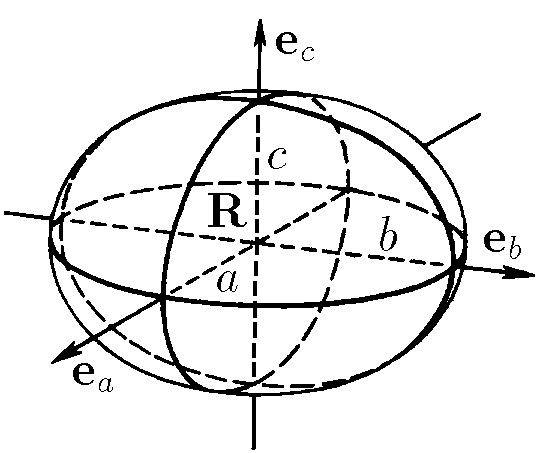
\includegraphics[width=\textwidth,height=0.8\textwidth]{ELLIPSE.png}
   \caption{ellipsoid}
   \label{fig:opo_ell}
\end{subfigure}
\hfill
\begin{subfigure}[b]{.3\textwidth}
   \centering
   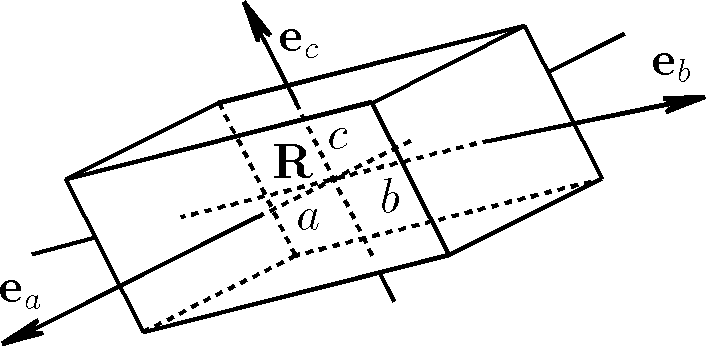
\includegraphics[width=\textwidth]{PAREPIP.png}
   \caption{parallelepiped}
   \label{fig:opo_parep}
\end{subfigure}
\hfill
\begin{subfigure}[b]{0.3\textwidth}
   \centering
   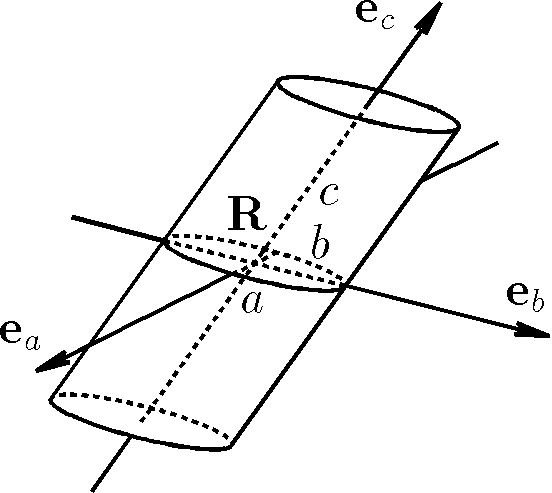
\includegraphics[width=\textwidth]{ZYLINDER.png}
   \caption{cylinder}
   \label{fig:opo_cyl}
\end{subfigure}
\caption{$\B{R}$: object center,
$a, b, c$: half axes/lengths,
$\B{e}_a$, $\B{e}_b$, $\B{e}_c$: directions of the half axes
}
\label{fig:opo}
\end{figure}

The scattering amplitude $F(\B{Q})$ of an object is given by the Fourier transform of the scattering length density distribution within the object
\begin{align}
F(\B{Q}) &= \int_V \mathrm{d}\B{r}\, \eta(\B{r})\, e^{\imath \B{Qr}},
\end{align}
where $\eta(\B{r})$ is the scattering length density distribution of the scattering object and $V$ the sample volume.
In the following it is assumed that the particles have a homogeneous scattering length density
$\eta_P$, embedded in a matrix of also homogeneous scattering length density $\eta_M = \eta_P-\Delta\eta$.
The position, orientation and size of the objects is uniquely defined by the center of scattering length density $\B{R}$, the half axes $a$, $b$ and $c$, as well as the direction of the half axes $\B{e}_a$, $\B{e}_b$ and
$\B{e}_c$. The base vectors $\B{e}_i$ are normalized $\abs{\B{e}_i}=1$ but do not need to be orthogonal to each other.  For the scattering amplitude of an individual objects one gets after a translation by $-\B{R}$ and a following change of basis $\M{D}$ from cartesian coordinates
$O_{xyz} = \{\B{e}_x, \B{e}_y,\B{e}_z\}$
into the coordinate system of the particle $O_{abc}=\{a\B{e}_a, b\B{e}_b,
c\B{e}_c\}$, so that $\B{P}_{O_{abc}} = \M{D}\, \B{P}_{O_{xyz}}$
\begin{align}
F(\B{Q}) &=
e^{-\imath\B{QR}}\, \Delta\eta\,
\int\limits_{V(\B{0})} \mathrm{d}\B{r}\, e^{\imath\B{Q}(\M{D}^{-1}\M{D}\B{r})}\\
%&=
%\det(\M{D}^{-1})\, e^{-\imath\B{QR}}\, \Delta\eta\,
%\int\limits_{\M{D} V(\B{0})} d\B{r}\, e^{\imath((\M{D}^{-1})^T\B{Q})\B{r}} \\
&=
\det(\M{D}^{-1})\, e^{-\imath\B{QR}}\, \Delta\eta\,
\int\limits_{\M{D} V(\B{0})} \mathrm{d}\B{r}\, e^{\imath \B{\hat{Q}}\B{r}}
\end{align}
with
\begin{align}
\displaystyle \B{\hat{Q}} = (\M{D}^{-1})^T\,\B{Q}
= \left( \begin{array}{l} a\,\B{e}_a\B{Q}\\ b\,\B{e}_b\B{Q}\\
c\, \B{e}_c\B{Q}
\end{array}\right)
\label{eq:Q:dach}
\end{align}
$V(\B{0})$ is the volume of the scattering object a scattering lenth density center located at the origin of the coordinate system and $\M{D} V(\B{0})$ is the volume of the unit object, i.e. unit sphere, unit cube or unit cylinder.
The transformation matrix $\M{D}$ and its inverse $\M{D}^{-1}$ are given by
\begin{align}
\M{D}^{-1} &=
\left(
\begin{array}{ccc}
a\, e_{ax} & b\, e_{bx} & c\, e_{cx} \\
a\, e_{ay} & b\, e_{by} & c\, e_{cy} \\
a\, e_{az} & b\, e_{bz} & c\, e_{cz} \\
\end{array}
\right) = (a\B{e}_a,b\B{e}_b,c\B{e}_c)\\
 \B{Q}(\M{D}^{-1}\B{r}) &= ((\M{D}^{-1})^T\B{Q})\B{r} \U{,}\\
\det(\M{D}^{-1}) &= abc\,
( e_{ax}\, e_{by}\, e_{cz}
+ e_{ay}\, e_{bz}\, e_{cx}
+ e_{az}\, e_{bx}\, e_{cy} \nonumber \\
&\phantom{=} - e_{az}\, e_{by}\, e_{cx}
   - e_{ay}\, e_{bx}\, e_{cz}
   - e_{ax}\, e_{bz}\, e_{cy})
\end{align}
\begin{align}
\M{D} &= (\M{D}^{-1})^{-1} = \frac{1}{\det(\M{D}^{-1})}\,
          (\M{D}^{-1})^{\rm adj} \nonumber \\
&= \frac{1}{\det(\M{D}^{-1})} \, (b\B{e}_b\times c\B{e}_c,-a\B{e}_a
\times c\B{e}_c,a\B{e}_a\times b\B{e}_b)
\end{align}
whereas $\det(\M{D}) \, \det(\M{D}^{-1}) = \det(\M{D}\, \M{D}^{-1}) =\det(\idty) = 1$

To reorient or rotate the objects one simply changes the  direction of the base vectors $\B{e}_a$, $\B{e}_b$, $\B{e}_c$ which is done by introducing a rotation matrix $\M{R}_{\alpha\beta\gamma}$. The rotation matrix can be defined via Euler angles $\alpha$, $\beta$,and $\gamma$. Its definition depends on the convention. There exist twelve possible sequences of rotation axes, divided in two groups: proper Euler angles ($z$-$x$-$z$, $x$-$y$-$x$, $y$-$z$-$y$, $z$-$y$-$z$, $x$-$z$-$x$, $y$-$x$-$y$),
Tait–Bryan angles ($x$-$y$-$z$, $y$-$z$-$x$, $z$-$x$-$y$, $x$-$z$-$y$, $z$-$y$-$x$, $y$-$x$-$z$). The difference between the two conventions is that Tait–Bryan angles represent rotations about three distinct axes, while proper Euler angles use the same axis for both the first and third elemental rotations. \SASfit allows internally to use any of the 12 conventions. However, as default conventions the yaw-pitch-roll is used (also named gier-nick-roll, east-north-up, north-East-Down, or $z$-$y$-$x$),  so that
\begin{align}
\displaystyle \B{\hat{Q}} &=
  \left( \begin{array}{l} a\,\M{R}_{\alpha\beta\gamma}\B{e}_a\B{Q}\\
                          b\,\M{R}_{\alpha\beta\gamma}\B{e}_b\B{Q}\\
                          c\,\M{R}_{\alpha\beta\gamma}\B{e}_c\B{Q}
\end{array}\right)
\label{eq:Q:dach}
\end{align}
\vspace{5mm}

Next to the form factor of an oriented primitive object also the form factor of it fully randomly oriented version is made available. The orientational average is done by integrating over the full Ewald's sphere, which is a double integration. \SASfit supplies for this orientational average separate integration routines which can be configured via the GUI. Next to the multidimensional adaptive integration routines \texttt{pcubature} and \texttt{hcubature} from \cite{Johnson} also some other routines are supplied, which however are nonadaptive without error estimate of the integral but optimized for integrations over a sphere surface. Nevertheless, these routines often need significant less function evaluations than a conventional multidimensional integration routines. The implemented methods are a 2D-GaussLegendre integration, Lebedev \cite{Lebedev1975,Lebedev1976,Lebedev1977} and Fibonacci \cite{Niederreiter1992,Marques2013} quadrature algorithm with a fixed and configurable number of function evaluations and without error estimation of the integral.

\subsection{perfect and random oriented ellipsoid} ~\\

\begin{figure}[htb]
\begin{center}
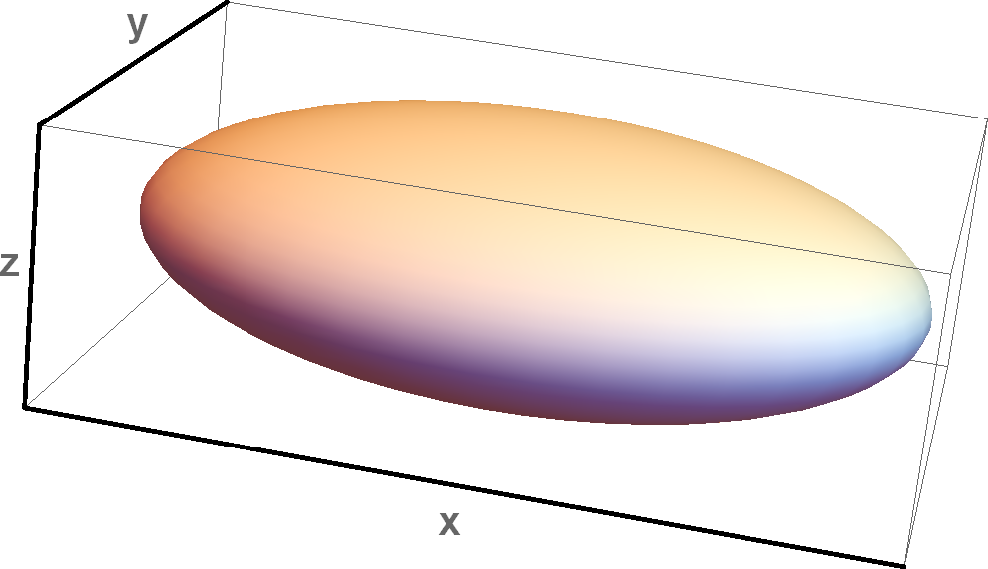
\includegraphics[width=0.65\textwidth]{../images/form_factor/supershapes/triaxial_ellipsoid321.png}
\end{center}
\caption{ellipsoid with semi-axis $(a:b:c)=(3:2:1)$ and $\alpha=\beta=\gamma=0$}
\label{fig:opo_ellipsoid}
\end{figure}

This form factor describes an oblique ellipsoid with half axis $a$, $b$, and $c$, which is obtained by an affine transformation of an unit sphere. The detector plane is in the $xy$-plane and the incident beam in the $-z$-direction. The unit vectors $\B{e}_a$, $\B{e}_b$, and $\B{e}_c$ are assumed in this example pointing into the directions of the three orthogonal axis $\B{e}_x$, $\B{e}_y$, and $\B{e}_z$ and therefore represent a triaxial ellipsoid.


\begin{align}
F_\mathrm{E}(\B{Q}) &=
\det(\M{D}^{-1})\, e^{-\imath\B{QR}}\, \Delta\eta\, \int\limits_0^1
\mathrm{d}r\, r^2 \int\limits_0^{\pi} \mathrm{d}\theta\, \sin \theta \int\limits_0^{2\pi}
\mathrm{d}\phi \, e^{\imath\B{\hat{Q}r}} \nonumber \\
&=
\displaystyle 4\, \pi\, \det(\M{D}^{-1})\, e^{-\imath\B{QR}}\,
\Delta\eta\, \frac{\sin \abs{\B{\hat{Q}}}-
\abs{\B{\hat{Q}}}\cos \abs{\B{\hat{Q}}}}{\abs{\B{\hat{Q}}}^3}
\label{eq:form:E}
\end{align}
For a random oriented ellipsoid one either can integrate over all Euler-angle, which is a tripple integration or over all orientations of $\B{Q}$, which is a double integration and performed for the randomized form factor. The corresponding scattering amplitude $F_{\mathrm{E},rnd}$ and scattering intensity $P_{\mathrm{E},rnd}$ are then given by
\begin{align}
F_{\mathrm{E,rnd}}(Q) &= \left\langle F_\mathrm{E}(\B{Q})\right\rangle_\B{Q} = \int_0^\pi\mathrm{d}\theta \int_0^{2\pi}\mathrm{d}\phi \; F_E\left(Q\begin{pmatrix}
                                       \cos(\phi)\sin(\theta) \\
                                       \sin(\phi)\sin(\theta) \\
                                       \cos(\theta)
                                     \end{pmatrix}\right) \\
P_{\mathrm{E,rnd}}(Q) &= \left\langle F_\mathrm{E}^2(\B{Q})\right\rangle_\B{Q} = \int_0^\pi\mathrm{d}\theta \int_0^{2\pi}\mathrm{d}\phi \; F_E^2\left(Q\begin{pmatrix}
                                       \cos(\phi)\sin(\theta) \\
                                       \sin(\phi)\sin(\theta) \\
                                       \cos(\theta)
                                     \end{pmatrix}\right)
\end{align}

\begin{figure}[htb]
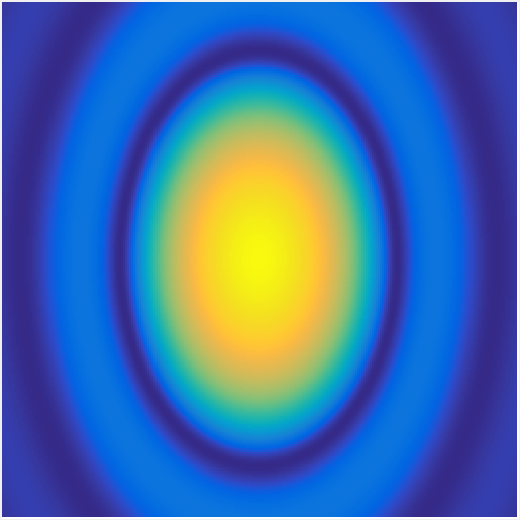
\includegraphics[width=0.31\textwidth]{../images/form_factor/supershapes/ellipsoid_0_0_0_18m.png} \hfill
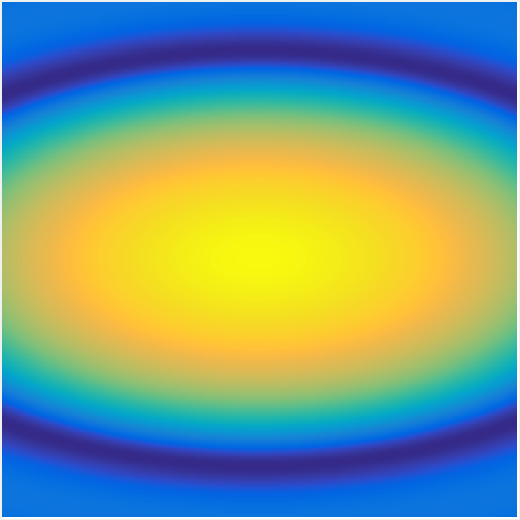
\includegraphics[width=0.31\textwidth]{../images/form_factor/supershapes/ellipsoid_0_90_0_18m.png}  \hfill 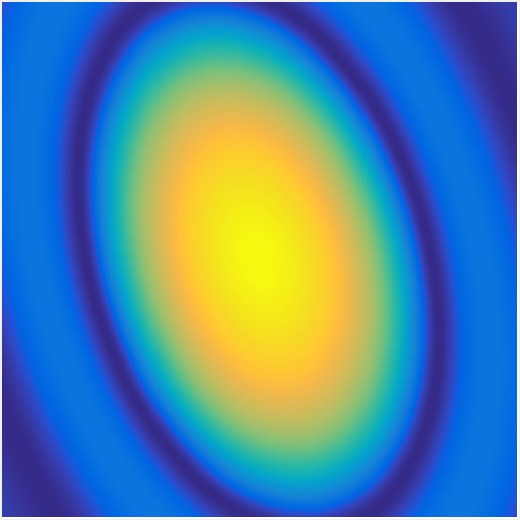
\includegraphics[width=0.31\textwidth]{../images/form_factor/supershapes/ellipsoid_0_45_45_18m.png}
\caption{Scattering patterns at 18m detector distance and a wavelength of $\lambda=0.6$nm. The ellipsoids are simulated with radii of $a=30$nm, $b=20$nm, and $c=10$nm. The Tait–Bryan angles (yaw-pitch-roll) are $(\alpha=0^\circ,\beta=0^\circ,\gamma=0^\circ)$, $(\alpha=0^\circ,\beta=90^\circ,\gamma=0^\circ)$, and $(\alpha=0^\circ,\beta=45^\circ,\gamma=45^\circ)$ }
\label{fig:opo_ellipsoidIQ2D}
\end{figure}
~\\
\uline{Input Parameters for model \texttt{ellipsoid (opo)}:}
\begin{description}
\item[\texttt{a}] length of first half axis
\item[\texttt{ea\_x}] $x$-component of fist axis.
\item[\texttt{ea\_y}] $y$-component of fist axis.
\item[\texttt{ea\_z}] $z$-component of fist axis.
\item[\texttt{b}] length of second half axis
\item[\texttt{eb\_x}] $x$-component of second axis.
\item[\texttt{eb\_y}] $y$-component of second axis.
\item[\texttt{eb\_z}] $z$-component of second axis.
\item[\texttt{c}] length of third half axis
\item[\texttt{ec\_x}] $x$-component of third axis.
\item[\texttt{ec\_y}] $y$-component of third axis.
\item[\texttt{ec\_z}] $z$-component of third axis.
\item[\texttt{eta\_p}] scattering length density $\eta_p$ of particle
\item[\texttt{eta\_m}] scattering length density $\eta_m$ of matrix
\item[\texttt{alpha}] first Euler angle
\item[\texttt{beta}] second Euler angle
\item[\texttt{gamma}] third Euler angle
\item[\texttt{psi}] direction of $\B{Q}$ on detector ($\psi=0$, $x$-direction, to the right)
\end{description}


\begin{figure}[htb]
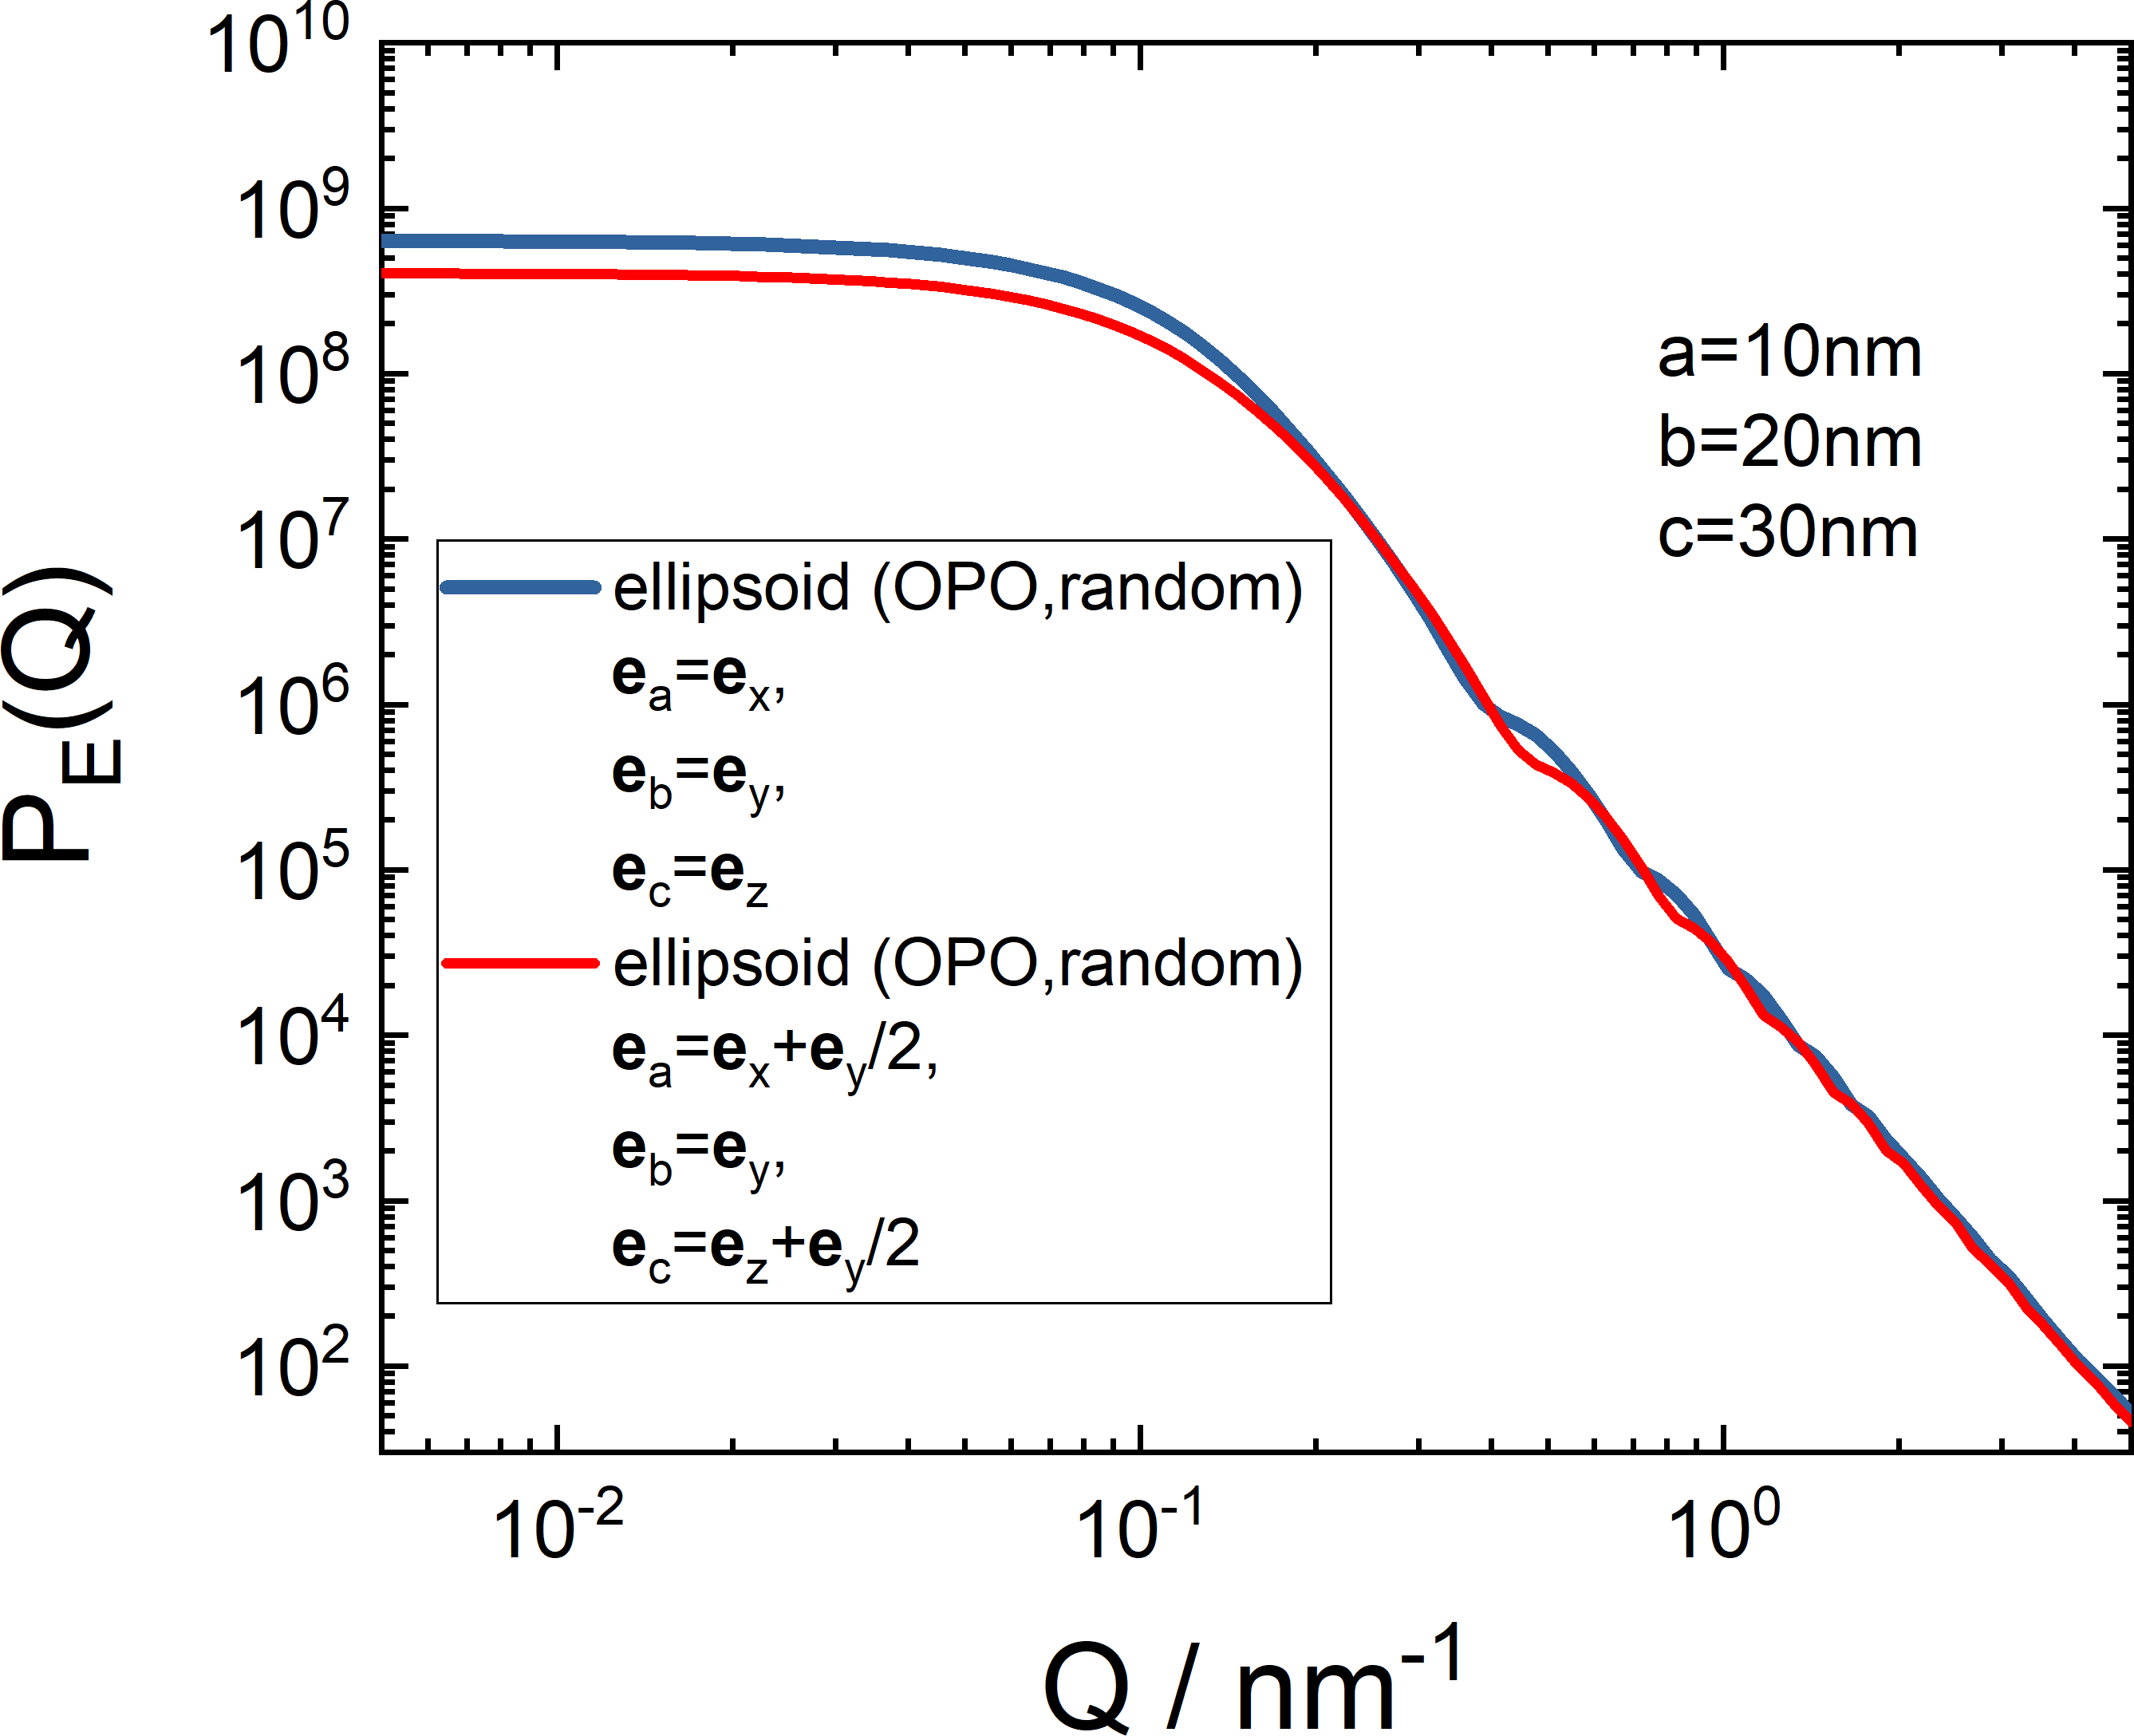
\includegraphics[width=0.481\textwidth]{../images/form_factor/oriented_primitive_opbjects/ellipsoidOPOoblique.png} \hfill
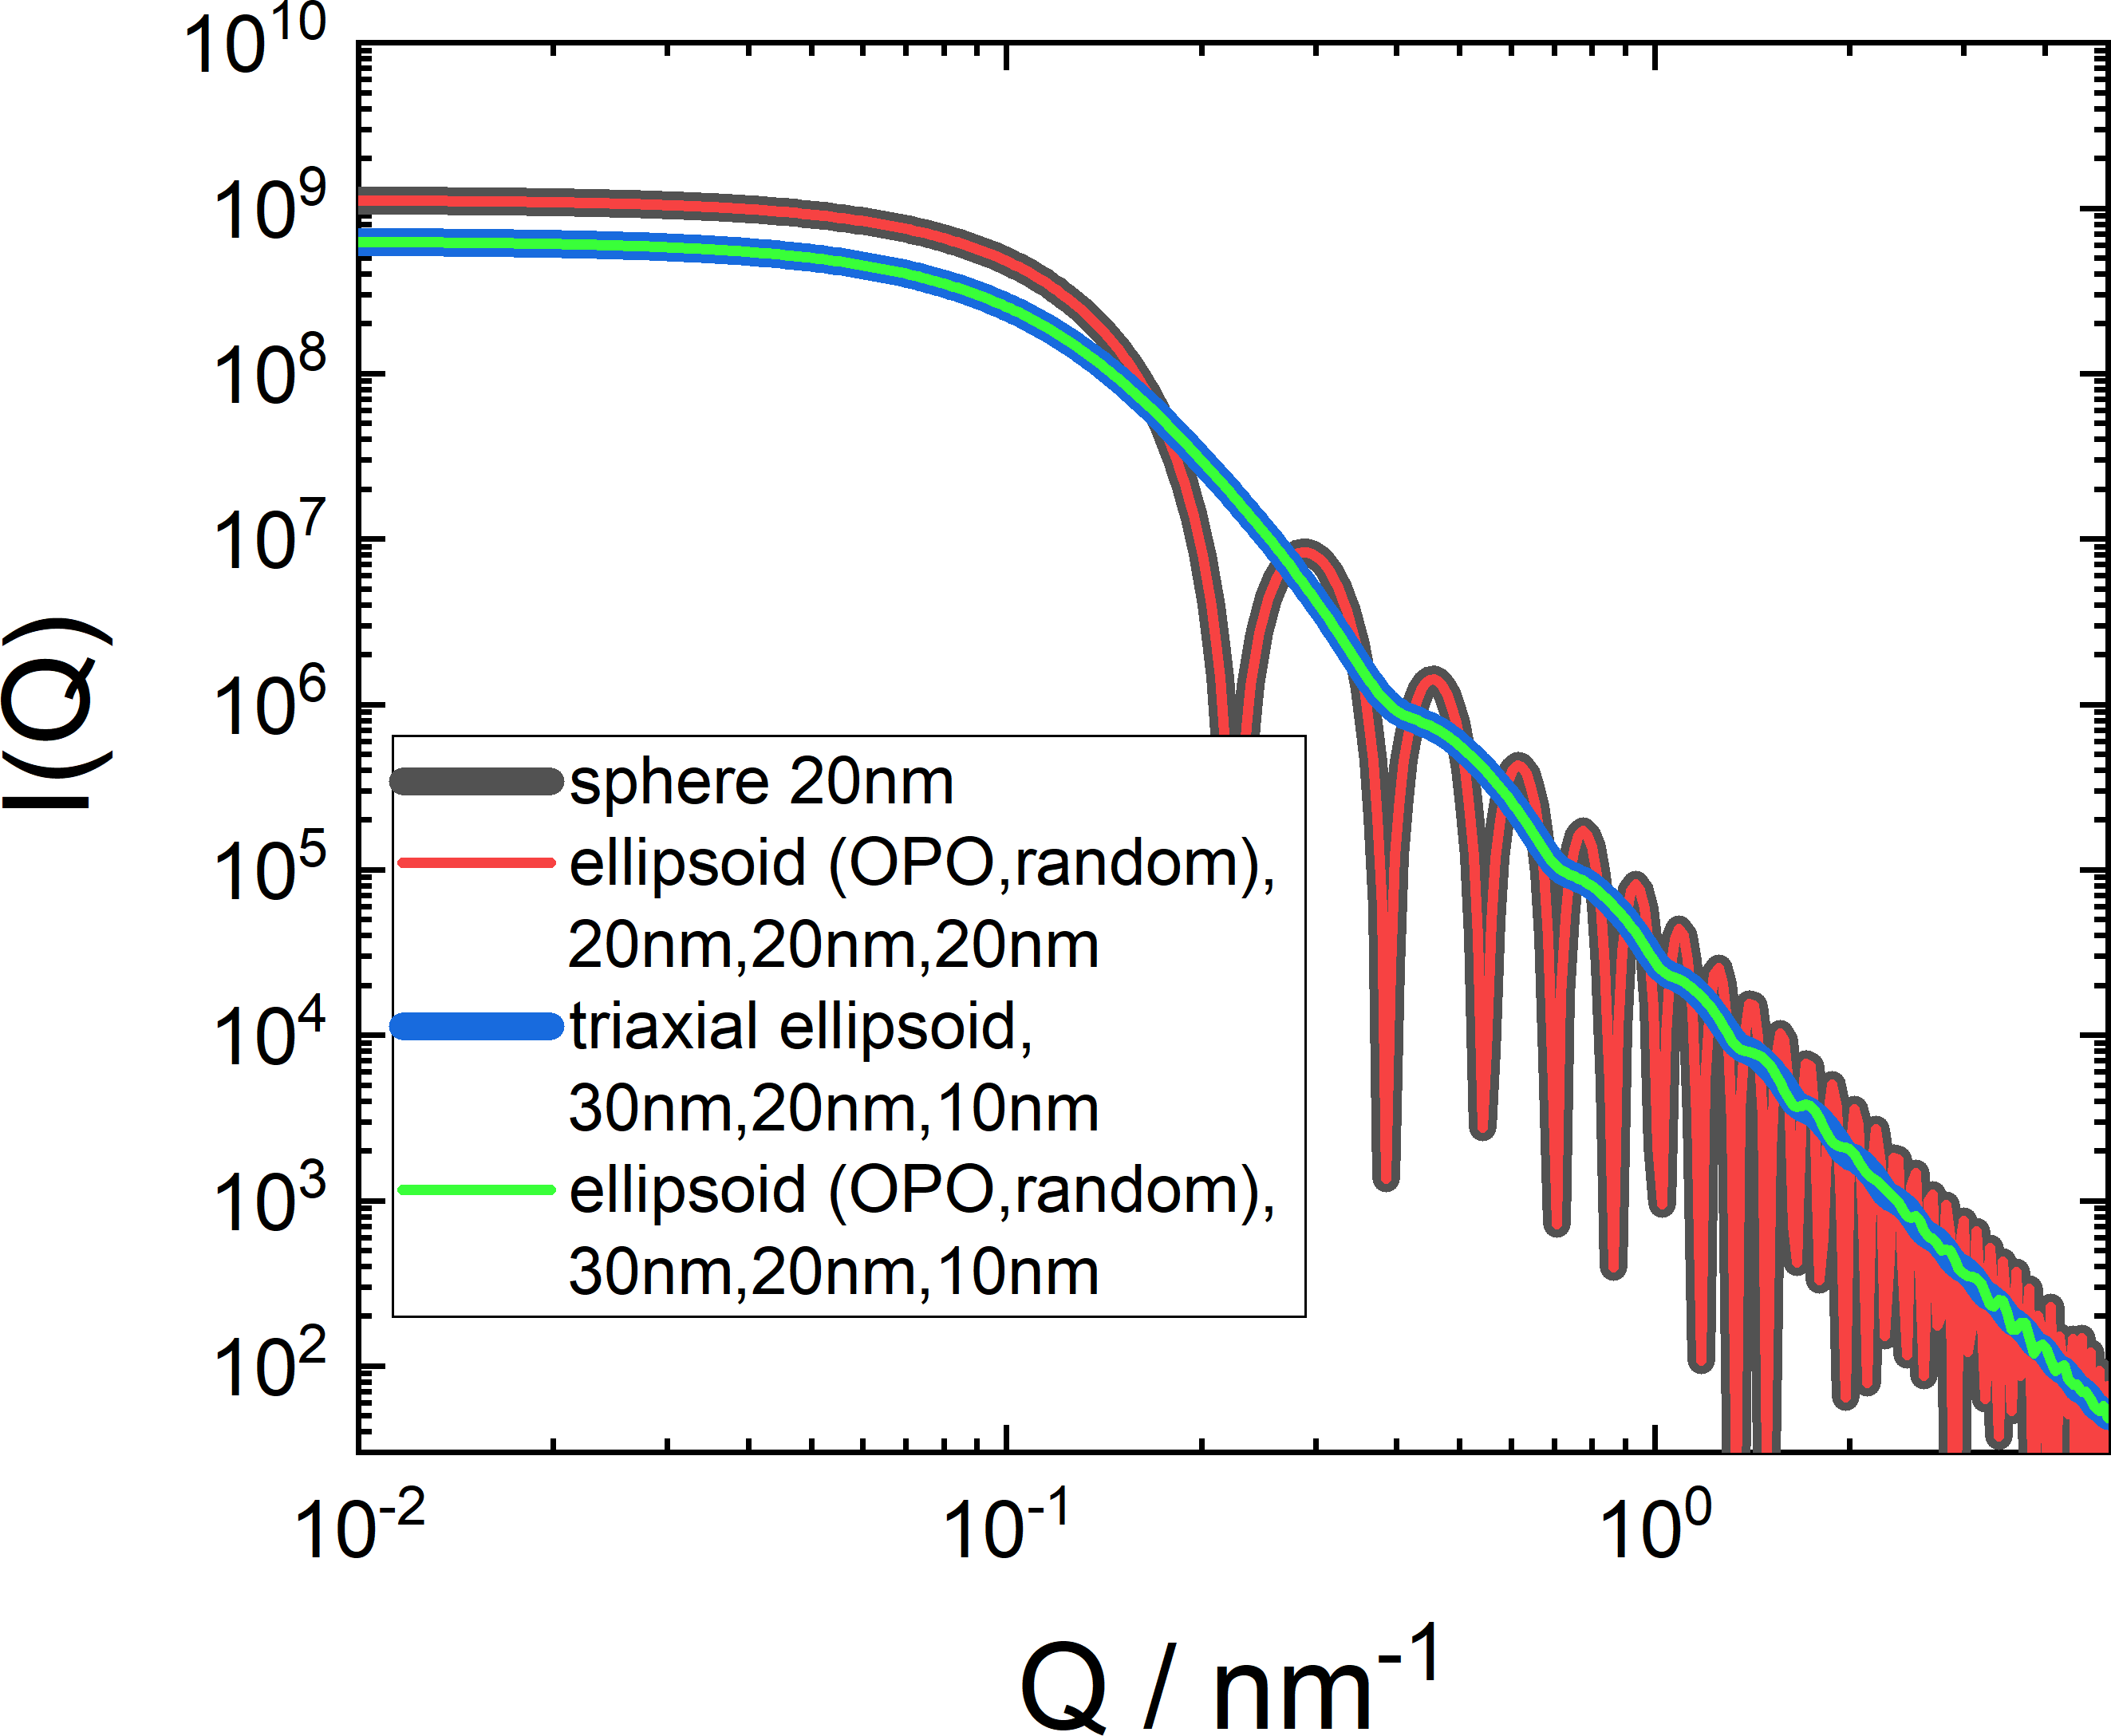
\includegraphics[width=0.481\textwidth]{../images/form_factor/oriented_primitive_opbjects/ellipsoidOPOcompare.png}
\caption{scattering curved of an oblique \texttt{ellipsoid (OPO,random)} (left) and a comparison with a sphere and a triaxial ellipsoid form factor (right)}
\label{fig:opo_ellipsoidIQrandom}
\end{figure}

~\\
\uline{Input Parameters for model \texttt{ellipsoid (opo, random)}:}
\begin{description}
\item[\texttt{a}] length of first half axis
\item[\texttt{ea\_x}] $x$-component of fist axis.
\item[\texttt{ea\_y}] $y$-component of fist axis.
\item[\texttt{ea\_z}] $z$-component of fist axis.
\item[\texttt{b}] length of second half axis
\item[\texttt{eb\_x}] $x$-component of second axis.
\item[\texttt{eb\_y}] $y$-component of second axis.
\item[\texttt{eb\_z}] $z$-component of second axis.
\item[\texttt{c}] length of third half axis
\item[\texttt{ec\_x}] $x$-component of third axis.
\item[\texttt{ec\_y}] $y$-component of third axis.
\item[\texttt{ec\_z}] $z$-component of third axis.
\item[\texttt{eta\_p}] scattering length density $\eta_p$ of particle
\item[\texttt{eta\_m}] scattering length density $\eta_m$ of matrix
\end{description}

\noindent\uline{Note:}
\begin{itemize}
\item the unit vector $\B{e}_a$, $\B{e}_b$, and $\B{e}_c$ are internally normalized to 1 and need to be linear independent.
\item the volume of the oblique ellipsoid is $V_\mathrm{E}=\frac43\det(\M{D}^{-1})$
\end{itemize}

\subsection{perfect and random oriented parallelepiped} ~\\

\begin{figure}[htb]
\begin{center}
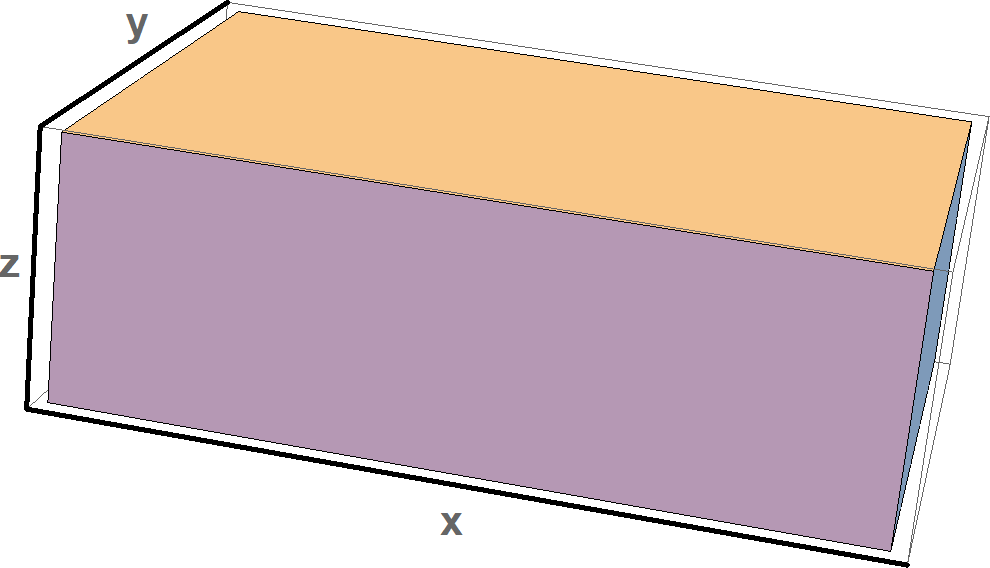
\includegraphics[width=0.6\textwidth]{../images/form_factor/supershapes/parallel_epiped321.png}
\end{center}
\caption{parallelepiped with half edge length $(a:b:c)=(3:2:1)$ and $\alpha=\beta=\gamma=0$}
\label{fig:opo_cube}
\end{figure}

This form factor describes an oblique parallelepiped which is obtained by an affine transformation of an unit cube with half edge lengths of $a$, $b$, and $c$. The detector plane is in the $xy$-plane and the incident beam in the $-z$-direction.


\begin{align}
F_\mathrm{P}(\B{Q}) &=
\det(\M{D}^{-1})\, e^{-\imath\B{QR}}\, \Delta\eta\, \int\limits_{-1}^1
\mathrm{d}x\, \int\limits_{-1}^{1} \mathrm{d}y\, \int\limits_{-1}^{1} \mathrm{d}z\,
e^{\imath\B{\hat{Q}r}} \nonumber \\
&= \displaystyle
8\, \det(\M{D}^{-1})\, e^{-\imath\B{QR}} \,\Delta\eta\,
\frac{\sin \B{\hat{Q}}\, \B{e}_x}{\B{\hat{Q}}\, \B{e}_x}
\,
\frac{\sin \B{\hat{Q}}\, \B{e}_y}{\B{\hat{Q}}\, \B{e}_y}
\,
\frac{\sin \B{\hat{Q}}\, \B{e}_z}{\B{\hat{Q}}\, \B{e}_z}
\label{eq:form:P}
\end{align}
For a random oriented parallelepiped the orientation average is done over all directions of $\B{Q}$. The corresponding scattering amplitude $F_{\mathrm{E},rnd}$ and scattering intensity $P_{\mathrm{E},rnd}$ are then given by
\begin{align}
F_{\mathrm{P,rnd}}(Q) &= \left\langle F_\mathrm{P}(\B{Q})\right\rangle_\B{Q} = \int_0^\pi\mathrm{d}\theta \int_0^{2\pi}\mathrm{d}\phi \; F_P\left(Q\begin{pmatrix}
                                       \cos(\phi)\sin(\theta) \\
                                       \sin(\phi)\sin(\theta) \\
                                       \cos(\theta)
                                     \end{pmatrix}\right) \\
P_{\mathrm{P,rnd}}(Q) &= \left\langle F_\mathrm{P}^2(\B{Q})\right\rangle_\B{Q} = \int_0^\pi\mathrm{d}\theta \int_0^{2\pi}\mathrm{d}\phi \; F_P^2\left(Q\begin{pmatrix}
                                       \cos(\phi)\sin(\theta) \\
                                       \sin(\phi)\sin(\theta) \\
                                       \cos(\theta)
                                     \end{pmatrix}\right)
\end{align}

\begin{figure}[htb]
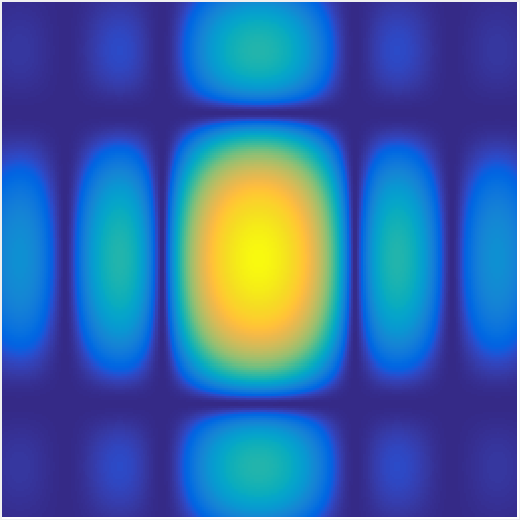
\includegraphics[width=0.31\textwidth]{../images/form_factor/supershapes/parallelepiped_0_0_0_18m.png}
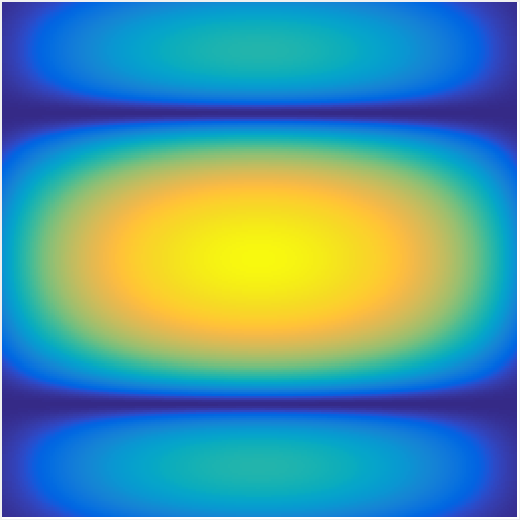
\includegraphics[width=0.31\textwidth]{../images/form_factor/supershapes/parallelepiped_0_90_0_18m.png}   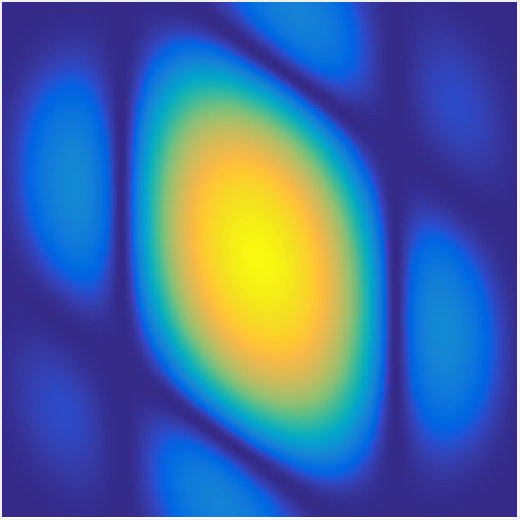
\includegraphics[width=0.31\textwidth]{../images/form_factor/supershapes/parallelepiped_0_45_45_18m.png}
\caption{Scattering patterns at 18m detector distance and a wavelength of $\lambda=0.6$nm. The parallelepipeds are simulated with half edge length of $a=30$nm, $b=20$nm, and $c=10$nm. The Tait–Bryan angles (yaw-pitch-roll) are $(\alpha=0^\circ,\beta=0^\circ,\gamma=0^\circ)$, $(\alpha=0^\circ,\beta=90^\circ,\gamma=0^\circ)$, and $(\alpha=0^\circ,\beta=45^\circ,\gamma=45^\circ)$ }
\label{fig:opo_parallelepipedIQ2D}
\end{figure}

~\\
\uline{Input Parameters for model \texttt{parallelepiped (opo)}:}
\begin{description}
\item[\texttt{a}] length of first half axis
\item[\texttt{ea\_x}] $x$-component of fist axis.
\item[\texttt{ea\_y}] $y$-component of fist axis.
\item[\texttt{ea\_z}] $z$-component of fist axis.
\item[\texttt{b}] length of second half axis
\item[\texttt{eb\_x}] $x$-component of second axis.
\item[\texttt{eb\_y}] $y$-component of second axis.
\item[\texttt{eb\_z}] $z$-component of second axis.
\item[\texttt{c}] length of third half axis
\item[\texttt{ec\_x}] $x$-component of third axis.
\item[\texttt{ec\_y}] $y$-component of third axis.
\item[\texttt{ec\_z}] $z$-component of third axis.
\item[\texttt{eta\_p}] scattering length density $\eta_p$ of particle
\item[\texttt{eta\_m}] scattering length density $\eta_m$ of matrix
\item[\texttt{alpha}] first Euler angle
\item[\texttt{beta}] second Euler angle
\item[\texttt{gamma}] third Euler angle
\item[\texttt{psi}] direction of $\B{Q}$ on detector ($\psi=0$, $x$-direction, to the right)
\end{description}

\begin{figure}[htb]
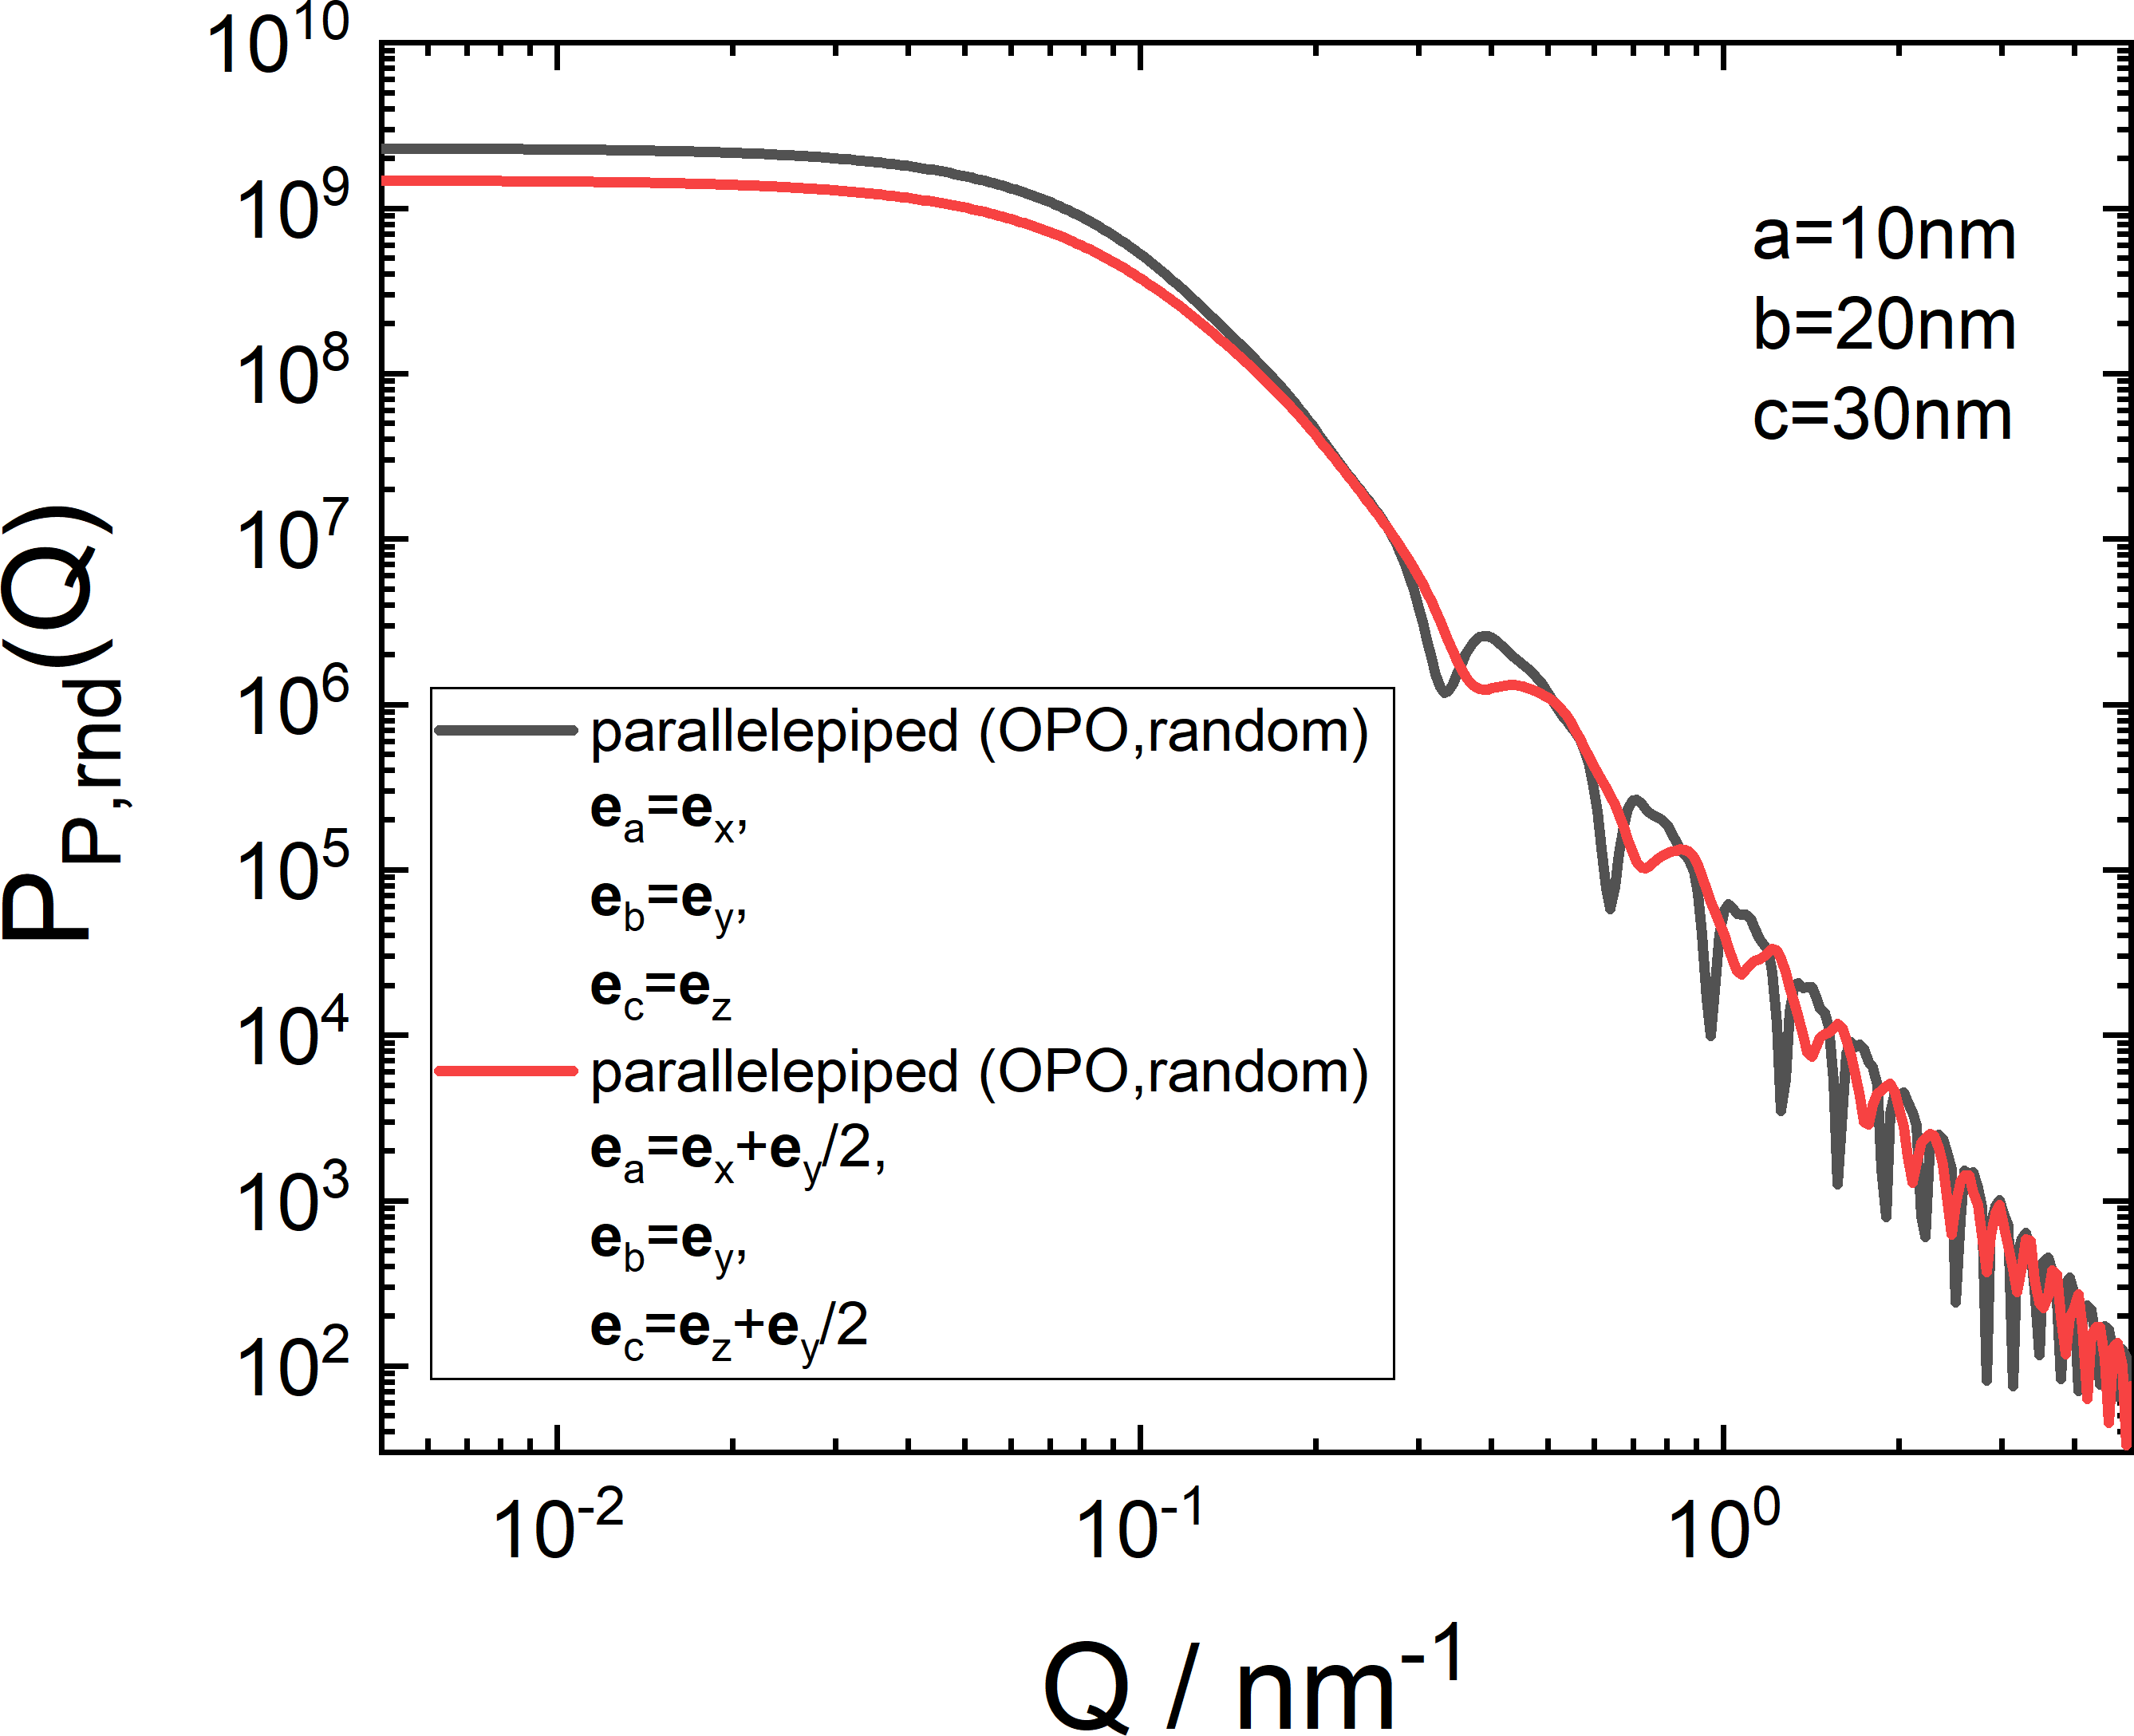
\includegraphics[width=0.481\textwidth]{../images/form_factor/oriented_primitive_opbjects/parallelepipedOPOoblique.png} \hfill
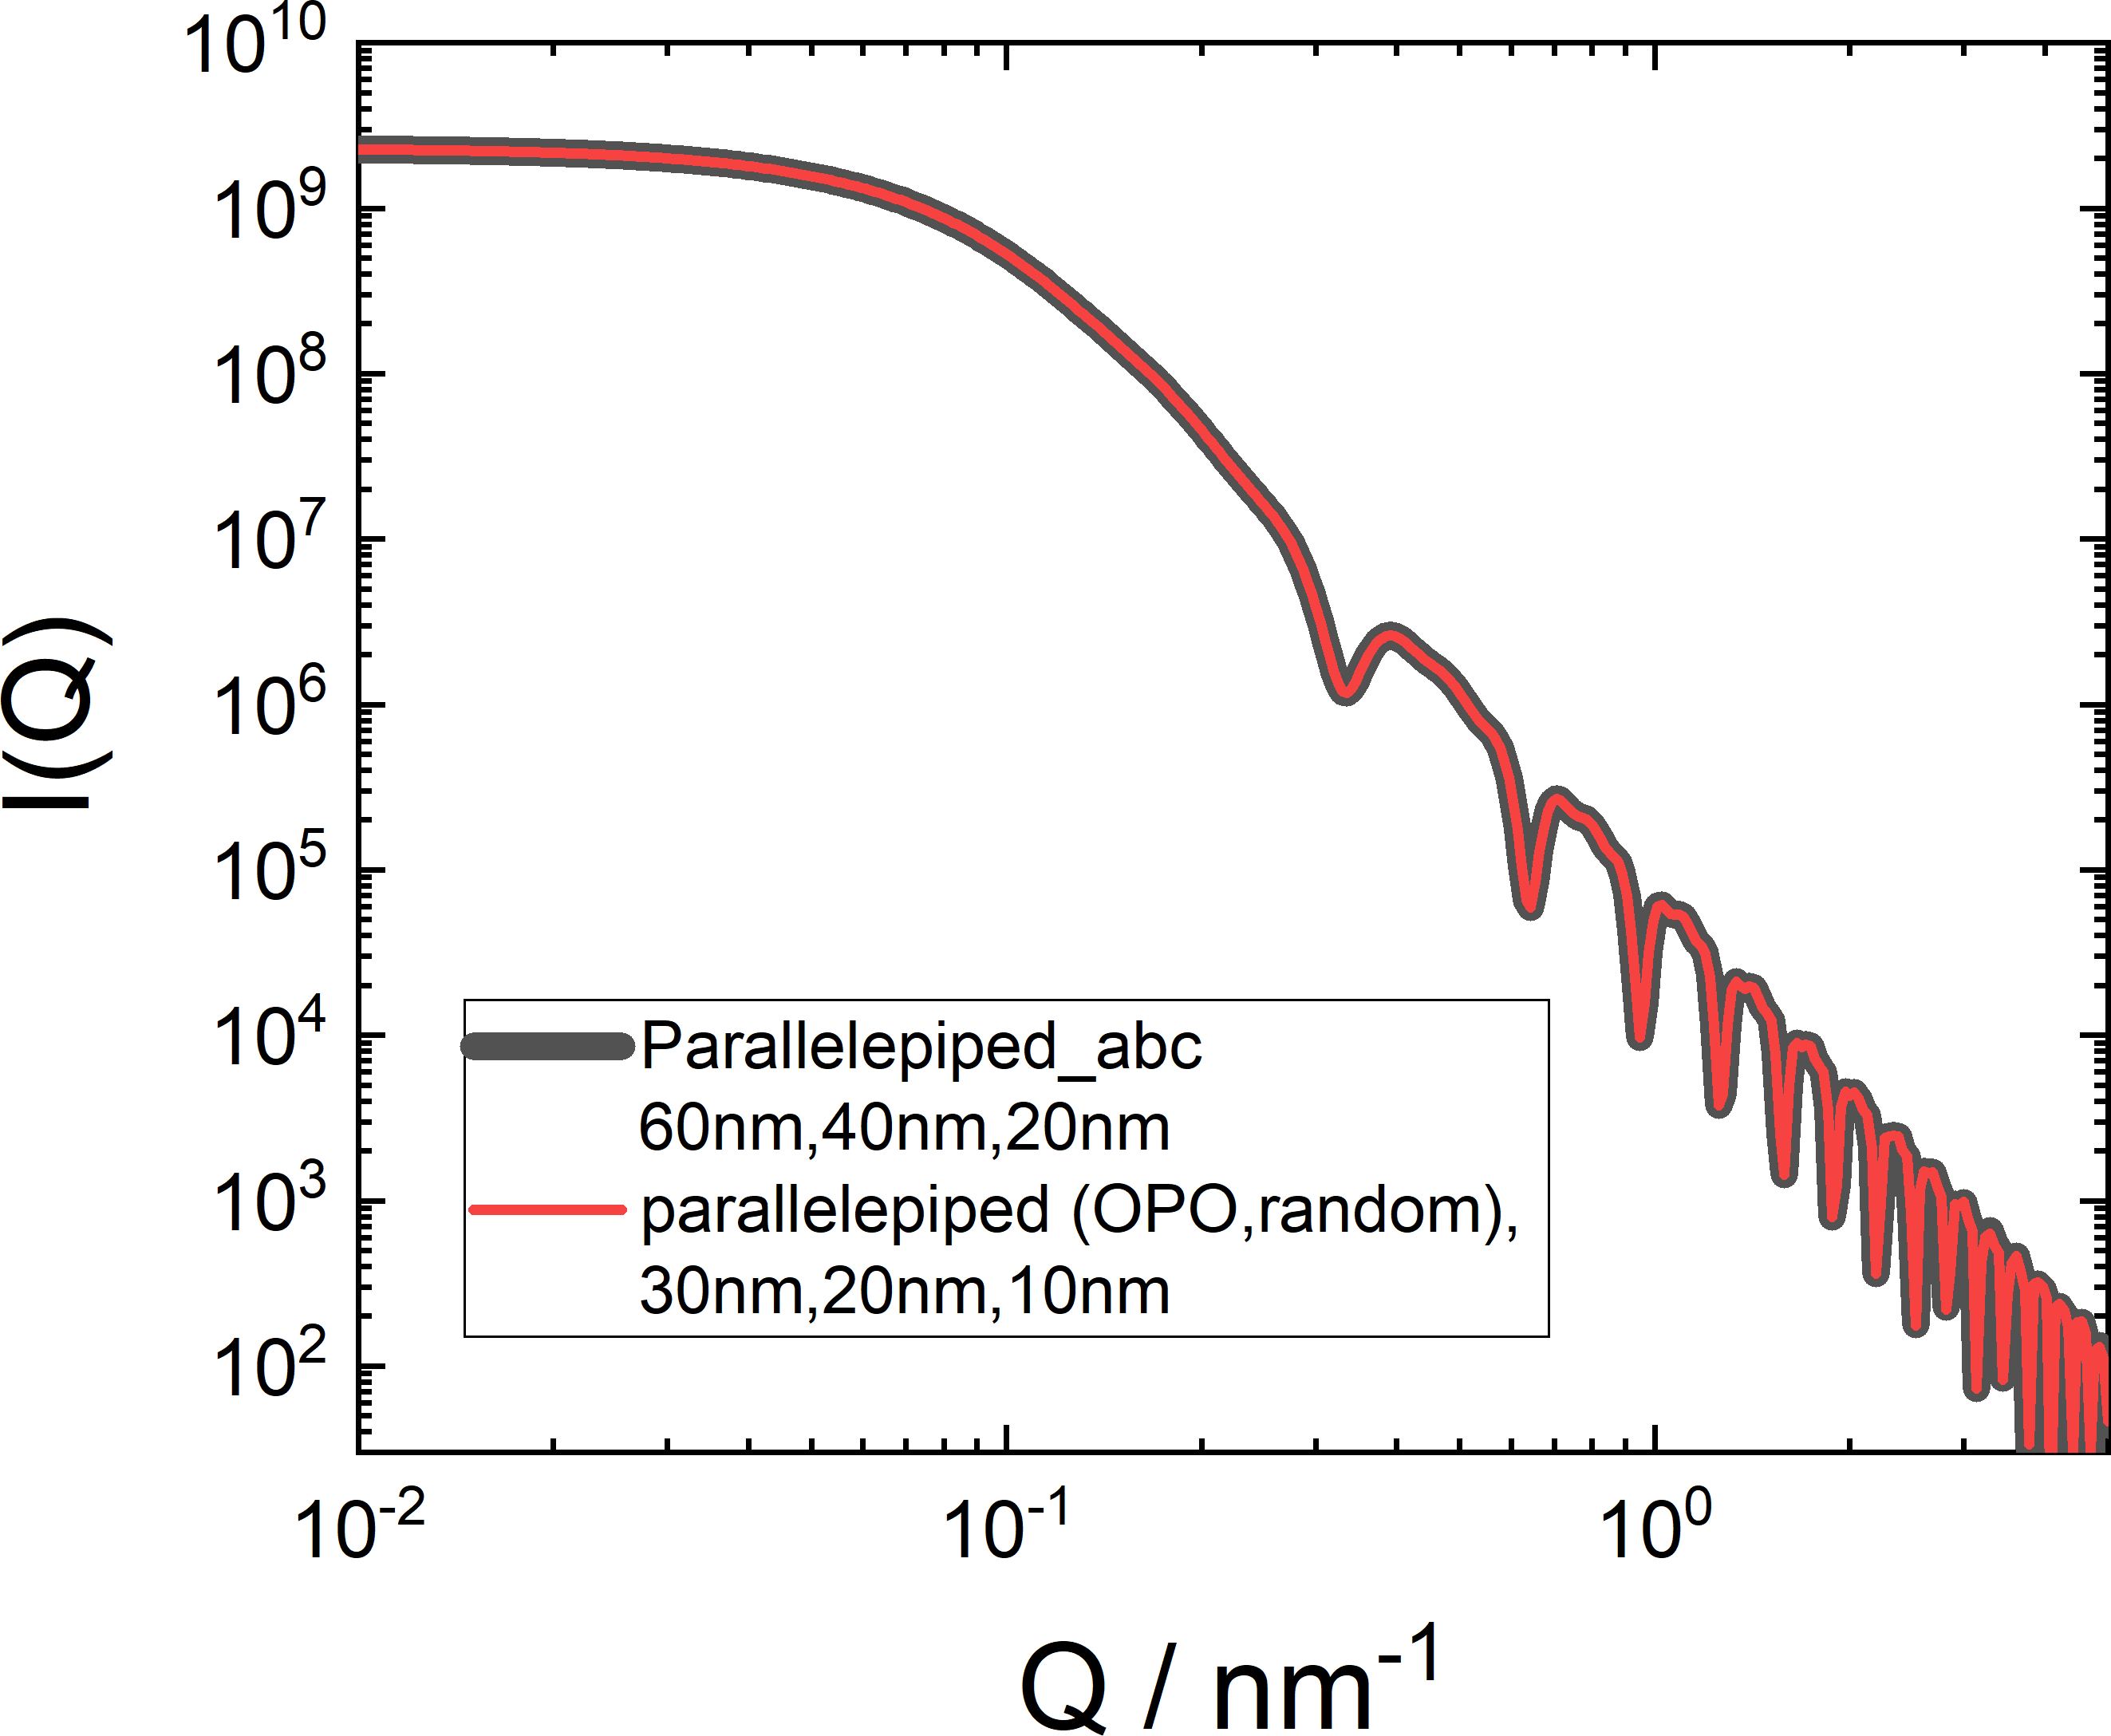
\includegraphics[width=0.481\textwidth]{../images/form_factor/oriented_primitive_opbjects/parallelepipedOPOcompare.png}
\caption{scattering curved of an oblique \texttt{parallelepiped (OPO,random)} (left) and a comparison of an \texttt{parallelepiped (OPO,random)} (using length of half axis) and \texttt{Parallelepiped\_abc} (using full edge length) form factor (right)}
\label{fig:opo_ellipsoidIQrandom}
\end{figure}

~\\
\uline{Input Parameters for model \texttt{parallelepiped (opo, random)}:}
\begin{description}
\item[\texttt{a}] length of first half axis
\item[\texttt{ea\_x}] $x$-component of fist axis.
\item[\texttt{ea\_y}] $y$-component of fist axis.
\item[\texttt{ea\_z}] $z$-component of fist axis.
\item[\texttt{b}] length of second half axis
\item[\texttt{eb\_x}] $x$-component of second axis.
\item[\texttt{eb\_y}] $y$-component of second axis.
\item[\texttt{eb\_z}] $z$-component of second axis.
\item[\texttt{c}] length of third half axis
\item[\texttt{ec\_x}] $x$-component of third axis.
\item[\texttt{ec\_y}] $y$-component of third axis.
\item[\texttt{ec\_z}] $z$-component of third axis.
\item[\texttt{eta\_p}] scattering length density $\eta_p$ of particle
\item[\texttt{eta\_m}] scattering length density $\eta_m$ of matrix
\end{description}

\noindent\uline{Note:}
\begin{itemize}
\item the unit vector $\B{e}_a$, $\B{e}_b$, and $\B{e}_c$ are internally normalized to 1 and need to be linear independent.
\item the volume of the oblique parallelepiped is $V_\mathrm{P}=8\det(\M{D}^{-1})$
\end{itemize}

\subsection{perfect and random oriented cylinder} ~\\

\begin{figure}[htb]
\begin{center}
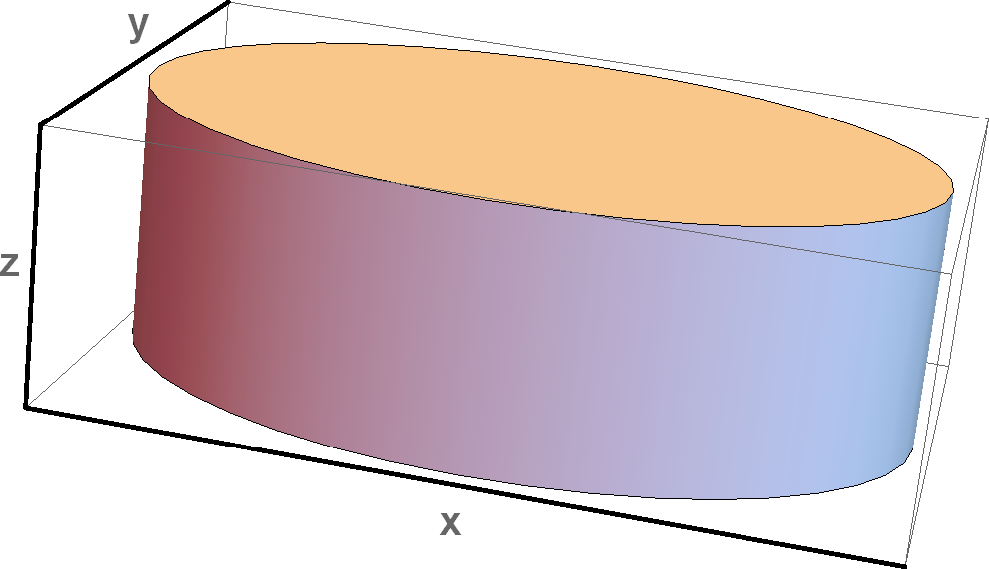
\includegraphics[width=0.6\textwidth]{../images/form_factor/supershapes/cylinder321.png}
\end{center}
\caption{cylinder with radii $a$ and $b$ and half height $c$. The axis ratios of the cylinder shown are $(a:b:c)=(3:2:1)$ and $\alpha=\beta=\gamma=0$}
\label{fig:opo_cylinder}
\end{figure}

This form factor describes an oblique cylinder which is obtained by an affine transformation of an unit cylinder with radii $a$ and $b$ and half height $c$. The detector plane is in the $xy$-plane and the incident beam in the $-z$-direction.


\begin{align}
F_C(\B{Q}) &=
\det(\M{D}^{-1})\, e^{-\imath\B{QR}}\, \Delta\eta\, \int\limits_{-1}^1
dz\, \int\limits_{0}^{1} dr\, r\, \int\limits_{0}^{2\pi} d\phi \,
e^{\imath\B{\hat{Q}r}} \nonumber \\
&=
4\, \pi\, \det(\M{D}^{-1})\, e^{-\imath\B{QR}}\, \Delta\eta\,
\frac{\sin\B{\hat{Q}e}_z}{\B{\hat{Q}e}_z}
\int\limits_{0}^1 dr\,r\,
\U{J}_0\left(r\, \sqrt{\left(\B{\hat{Q}}\B{e}_x\right)^2+
\left(\B{\hat{Q}}\B{e}_y\right)^2}\right)
\nonumber \\
&= \displaystyle
8\, \pi\,\det(\M{D}^{-1})\, e^{-\imath\B{QR}}\,
\Delta\eta\, \frac{\sin\B{\hat{Q}}\B{e}_z}{\B{\hat{Q}}\B{e}_z}
\, \frac{\U{J}_1\left(\sqrt{\left(\B{\hat{Q}}\B{e}_x\right)^2+
\left(\B{\hat{Q}}\B{e}_y\right)^2}\right)}{\sqrt{
\left(\B{\hat{Q}}\B{e}_x\right)^2+\left(\B{\hat{Q}}\B{e}_y\right)^2}}
\label{eq:form:C}
\end{align}

\begin{figure}[htb] 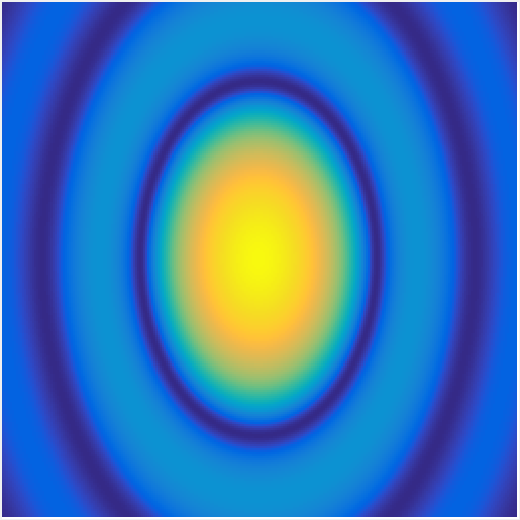
\includegraphics[width=0.31\textwidth]{../images/form_factor/supershapes/cylinder_0_0_0_18m.png}
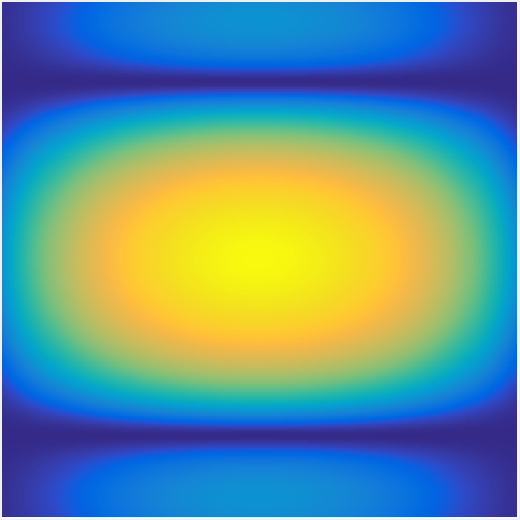
\includegraphics[width=0.31\textwidth]{../images/form_factor/supershapes/cylinder_0_90_0_18m.png}   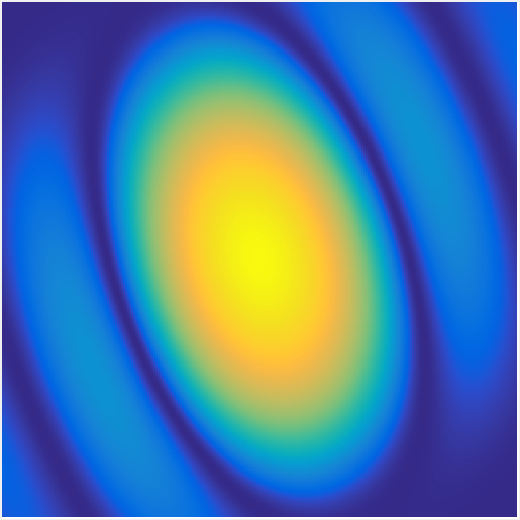
\includegraphics[width=0.31\textwidth]{../images/form_factor/supershapes/cylinder_0_45_45_18m.png}
\caption{Scattering patterns at 18m detector distance and a wavelength of $\lambda=0.6$nm. The cylinders are simulated with radii of $a=30$nm, $b=20$nm, and half height length $c=10$nm. The Tait–Bryan angles (yaw-pitch-roll) are $(\alpha=0^\circ,\beta=0^\circ,\gamma=0^\circ)$, $(\alpha=0^\circ,\beta=90^\circ,\gamma=0^\circ)$, and $(\alpha=0^\circ,\beta=45^\circ,\gamma=45^\circ)$ }
\label{fig:opo_cylinderIQ2D}
\end{figure}

For a random oriented oblique cylinder the orientation average is done over all directions of $\B{Q}$. The corresponding scattering amplitude $F_{\mathrm{C},rnd}$ and scattering intensity $P_{\mathrm{C},rnd}$ are then given by
\begin{align}
F_{\mathrm{C,rnd}}(Q) &= \left\langle F_\mathrm{C}(\B{Q})\right\rangle_\B{Q} = \int_0^\pi\mathrm{d}\theta \int_0^{2\pi}\mathrm{d}\phi \; F_\mathrm{C}\left(Q\begin{pmatrix}
                                       \cos(\phi)\sin(\theta) \\
                                       \sin(\phi)\sin(\theta) \\
                                       \cos(\theta)
                                     \end{pmatrix}\right) \\
P_{\mathrm{C,rnd}}(Q) &= \left\langle F_\mathrm{C}^2(\B{Q})\right\rangle_\B{Q} = \int_0^\pi\mathrm{d}\theta \int_0^{2\pi}\mathrm{d}\phi \; F_\mathrm{C}^2\left(Q\begin{pmatrix}
                                       \cos(\phi)\sin(\theta) \\
                                       \sin(\phi)\sin(\theta) \\
                                       \cos(\theta)
                                     \end{pmatrix}\right)
\end{align}
~\\
\uline{Input Parameters for model \texttt{cylinder (opo)}:}
\begin{description}
\item[\texttt{a}] length of first half axis
\item[\texttt{ea\_x}] $x$-component of fist axis.
\item[\texttt{ea\_y}] $y$-component of fist axis.
\item[\texttt{ea\_z}] $z$-component of fist axis.
\item[\texttt{b}] length of second half axis
\item[\texttt{eb\_x}] $x$-component of second axis.
\item[\texttt{eb\_y}] $y$-component of second axis.
\item[\texttt{eb\_z}] $z$-component of second axis.
\item[\texttt{c}] length of third half axis
\item[\texttt{ec\_x}] $x$-component of third axis.
\item[\texttt{ec\_y}] $y$-component of third axis.
\item[\texttt{ec\_z}] $z$-component of third axis.
\item[\texttt{eta\_p}] scattering length density $\eta_p$ of particle
\item[\texttt{eta\_m}] scattering length density $\eta_m$ of matrix
\item[\texttt{alpha}] first Euler angle
\item[\texttt{beta}] second Euler angle
\item[\texttt{gamma}] third Euler angle
\item[\texttt{psi}] direction of $\B{Q}$ on detector ($\psi=0$, $x$-direction, to the right)
\end{description}


\begin{figure}[htb]
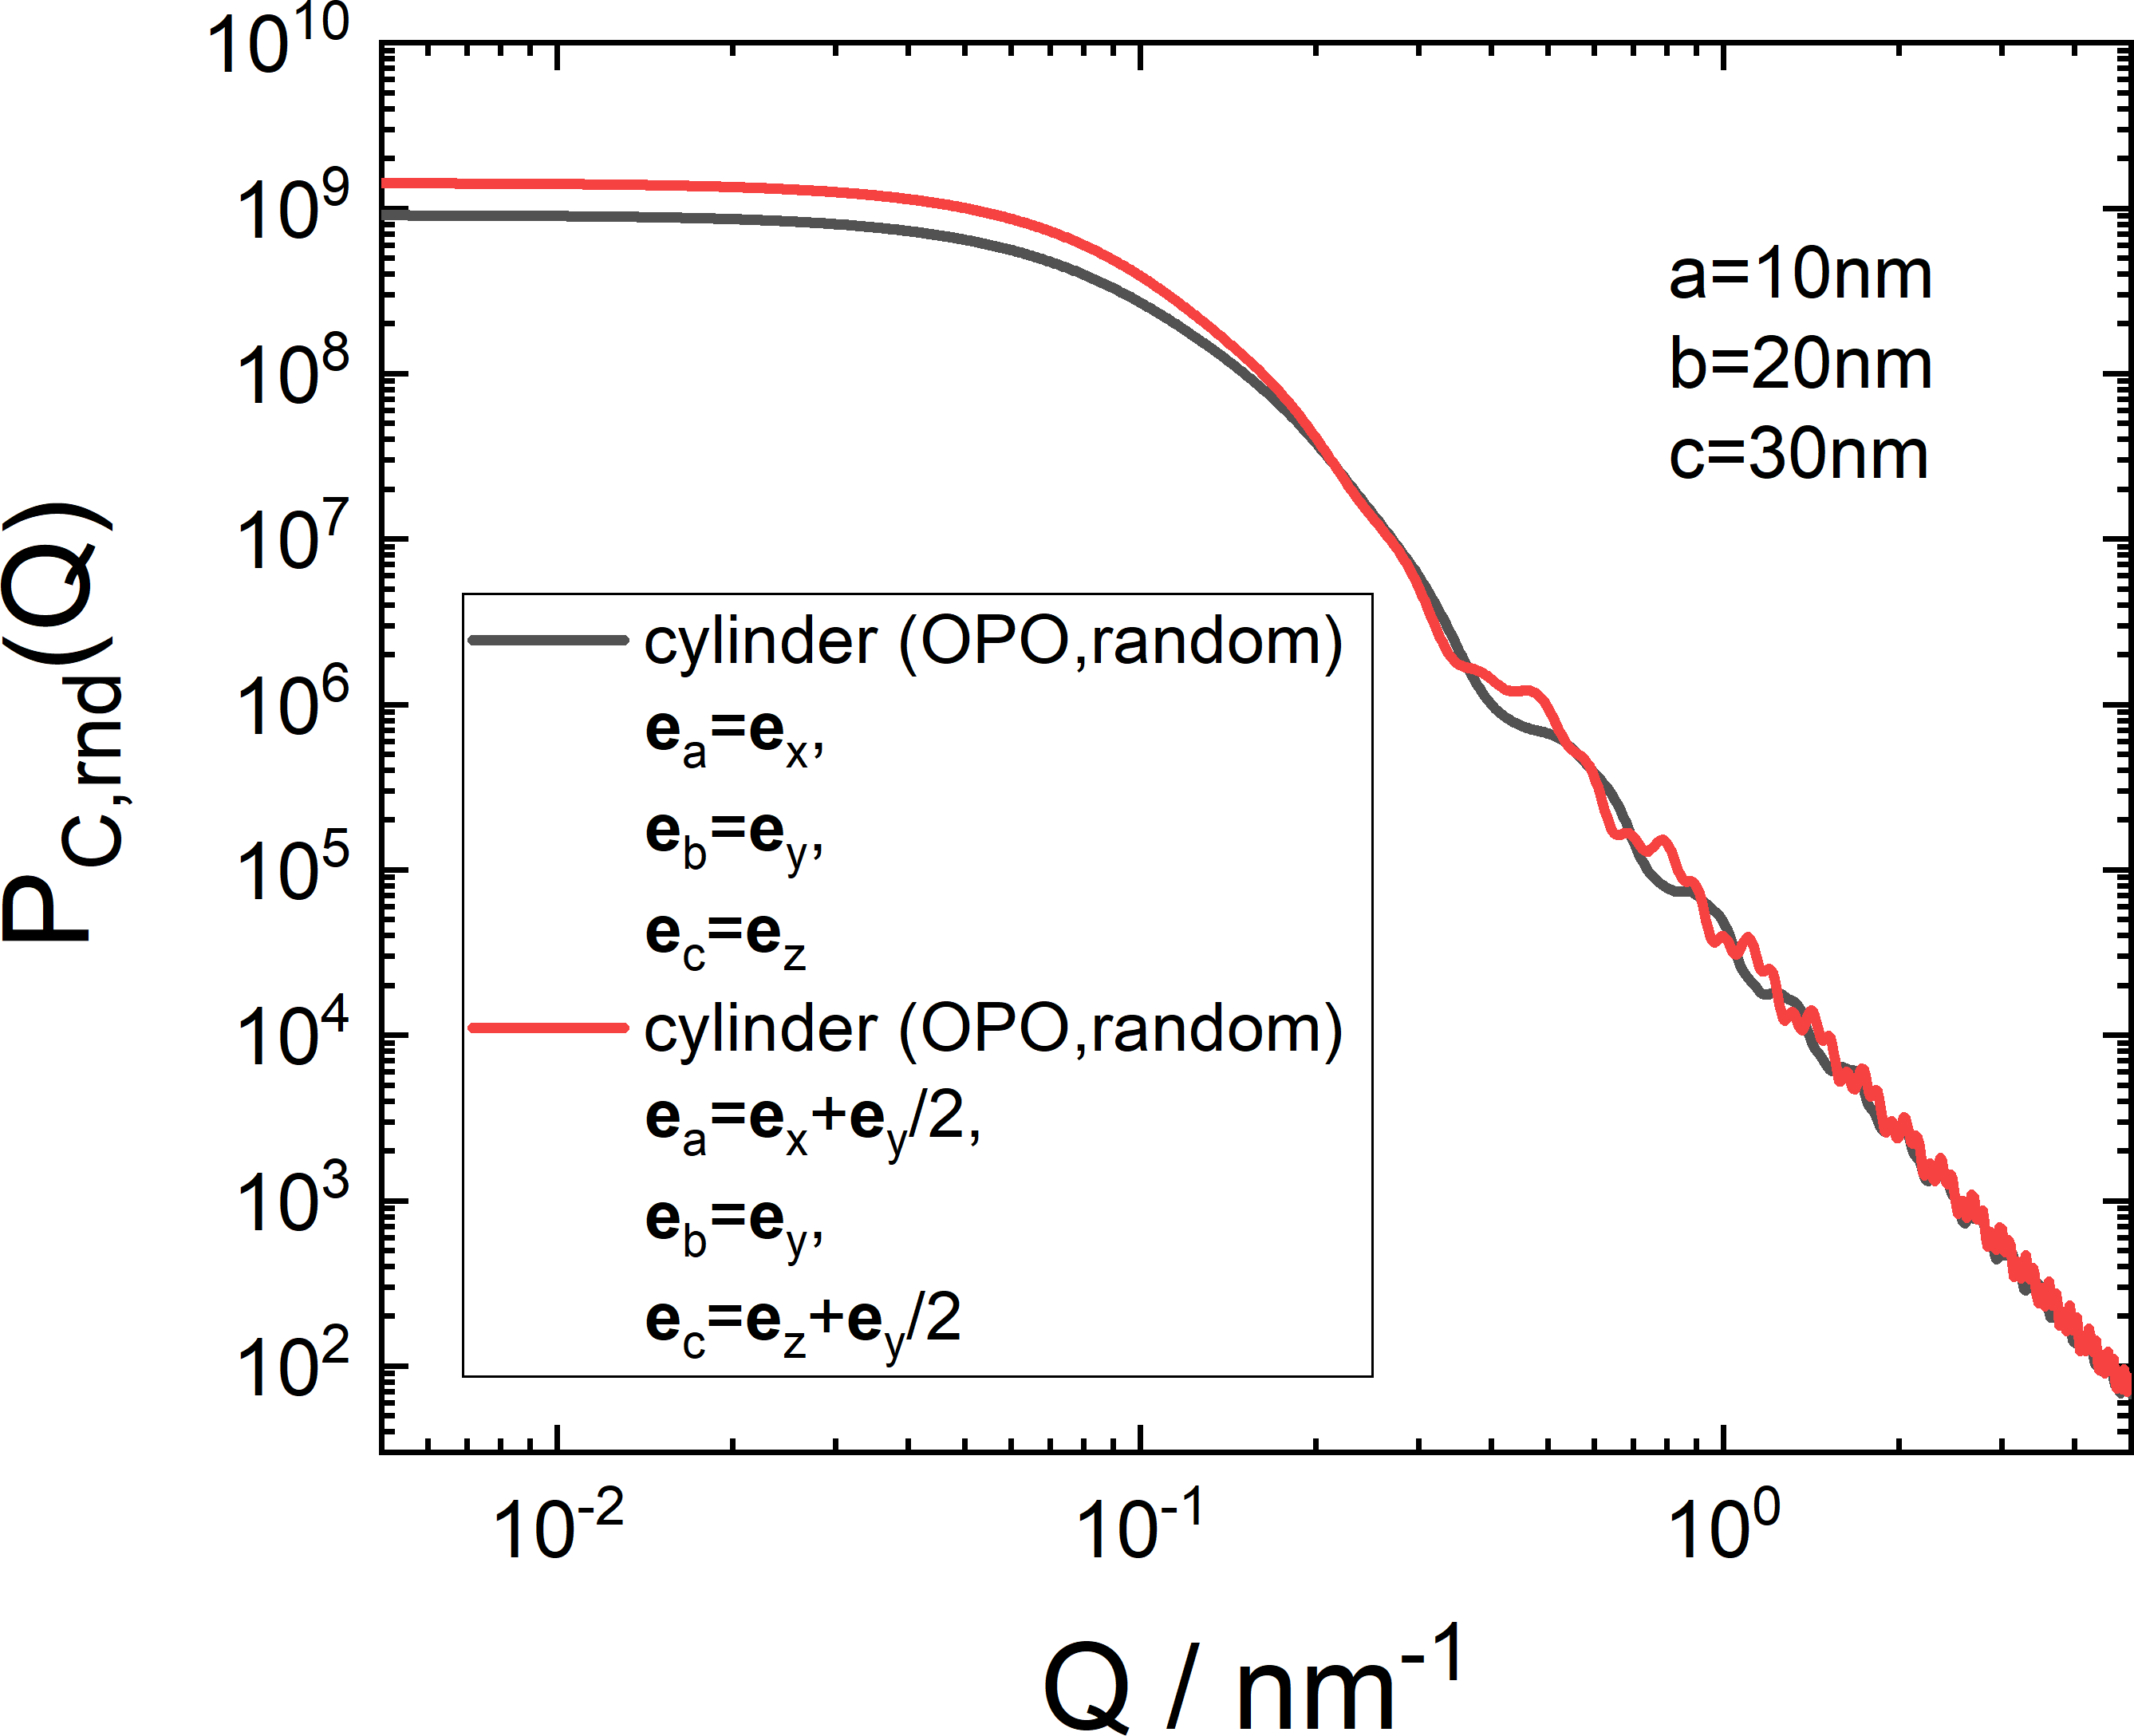
\includegraphics[width=0.481\textwidth]{../images/form_factor/oriented_primitive_opbjects/cylinderOPOoblique.png} \hfill
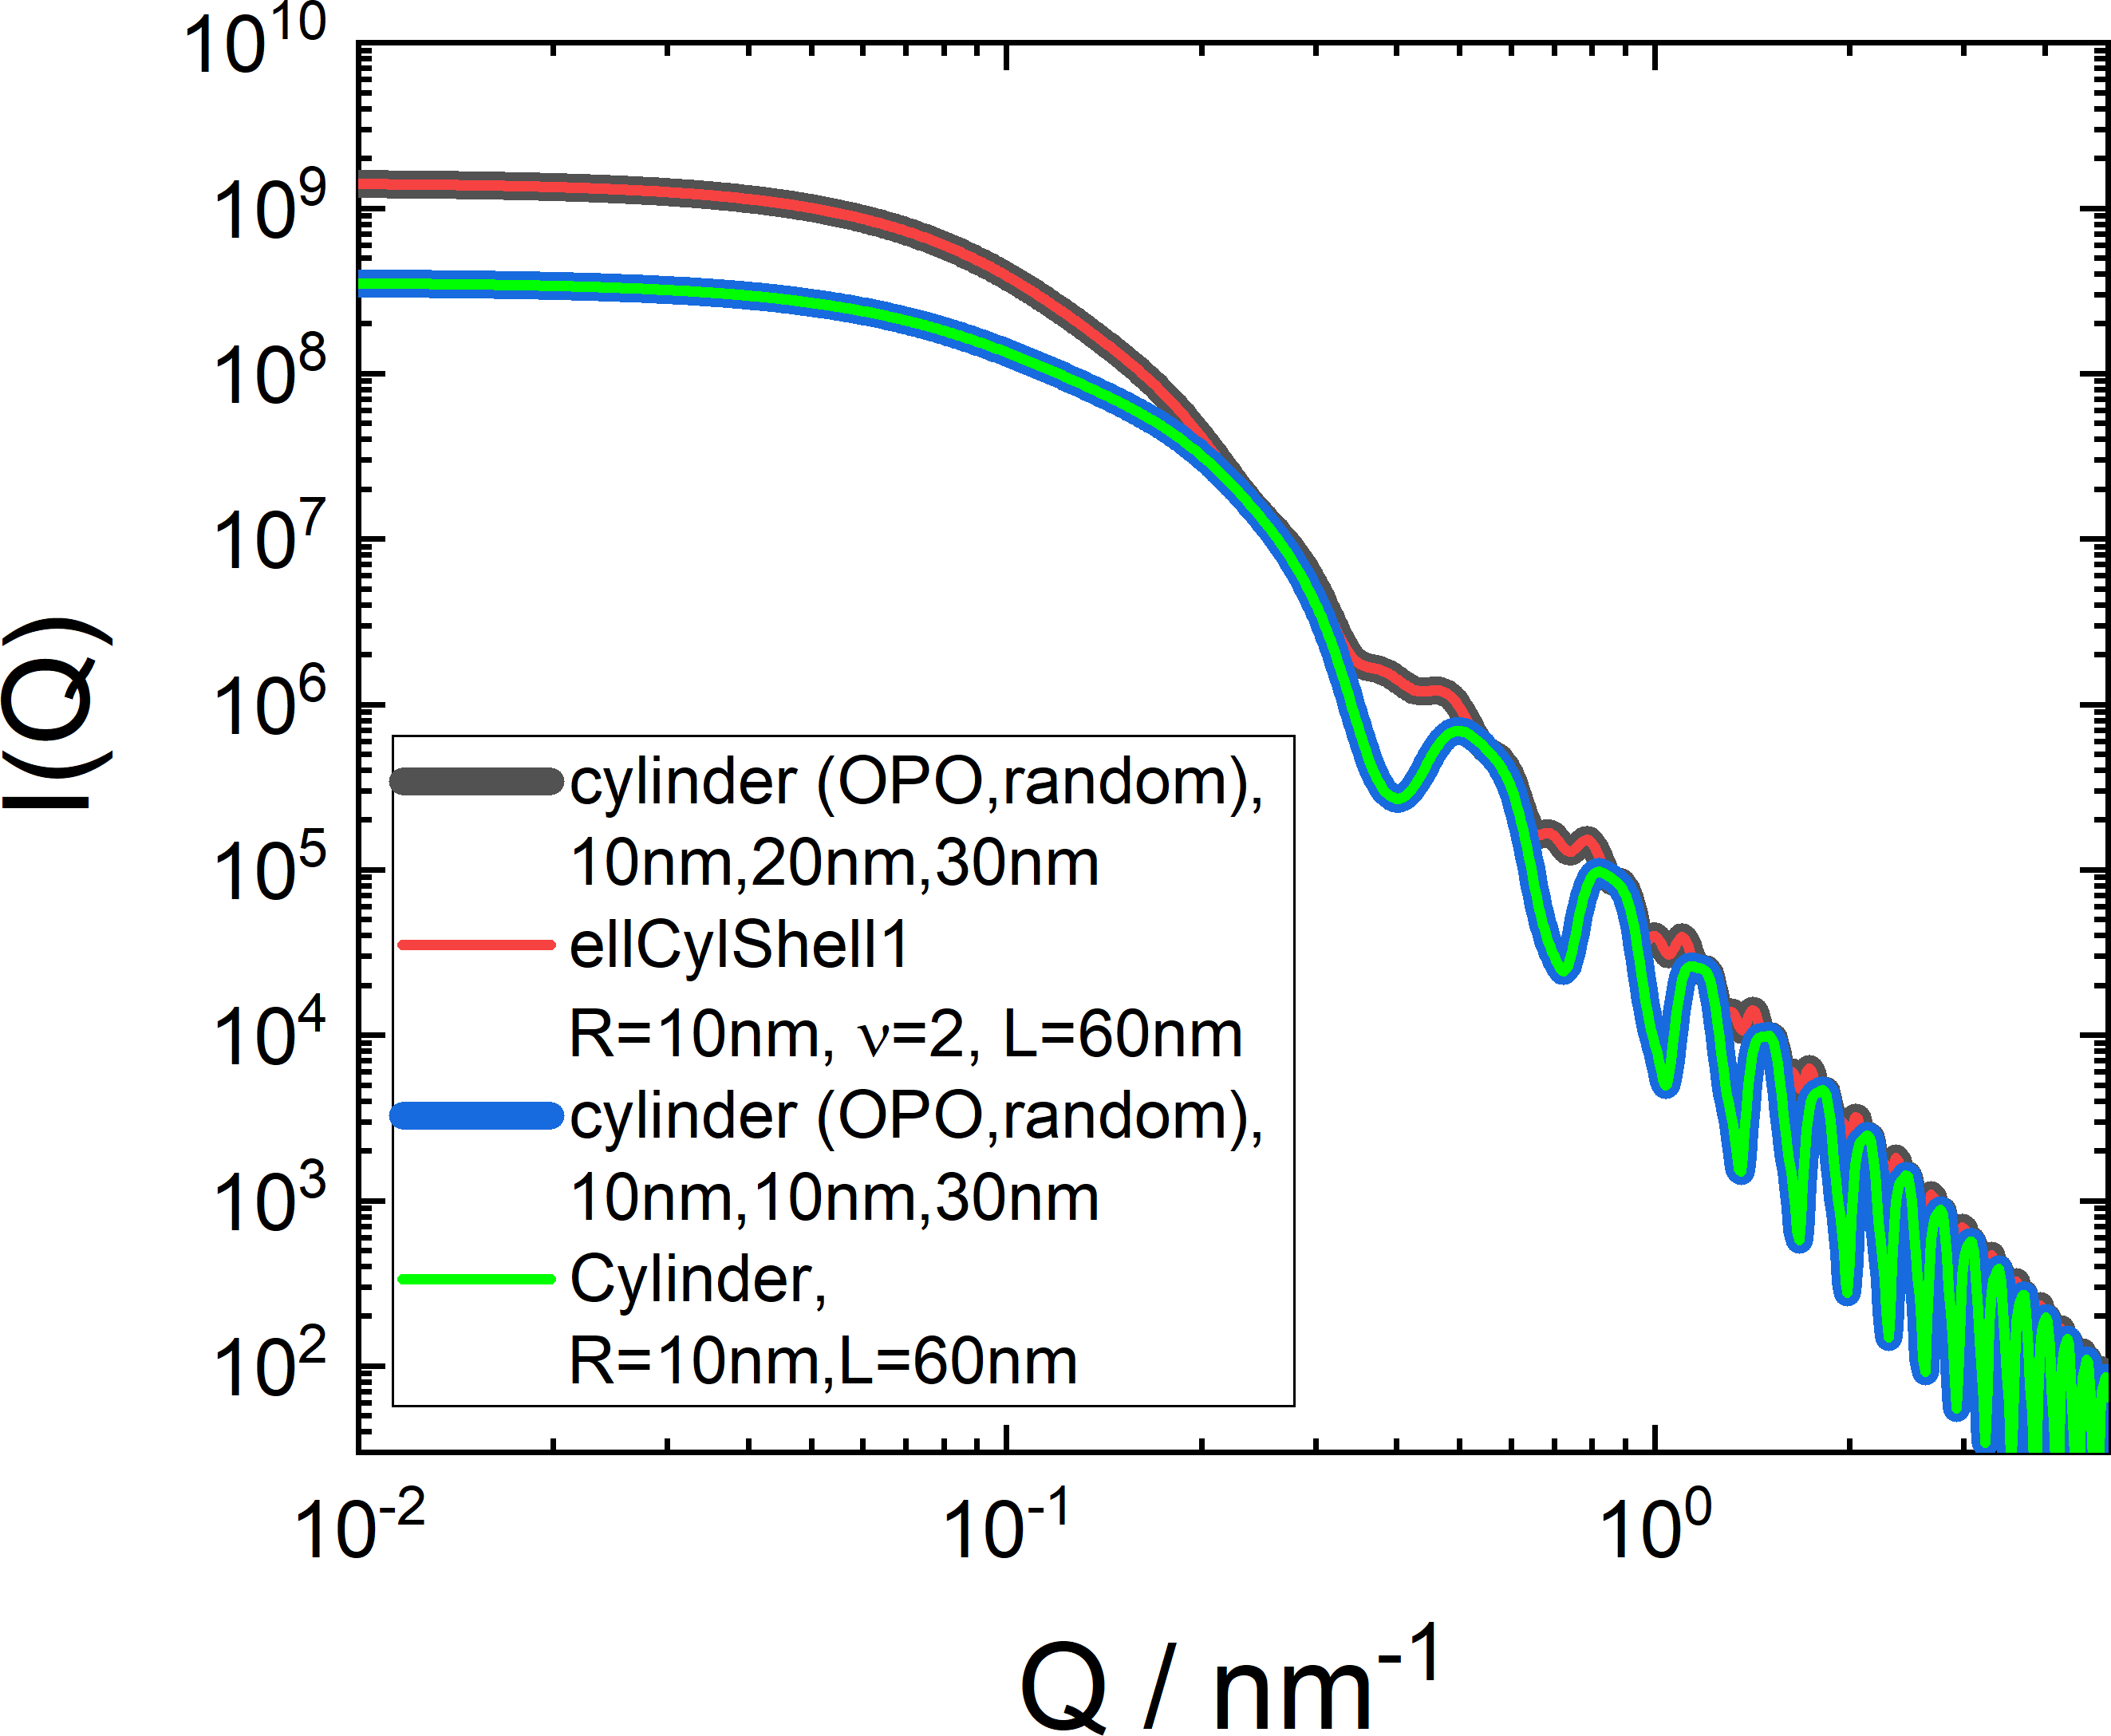
\includegraphics[width=0.481\textwidth]{../images/form_factor/oriented_primitive_opbjects/cylinderOPOcompare.png}
\caption{scattering curved of an oblique \texttt{cylinder (OPO,random)} (left) and a comparison of an \texttt{parallelepiped (OPO,random)} with an elliptical cylindrical shell \texttt{ellCylShell1} and a random oriented solid cylinder  \texttt{Cylinder} form factor (right)}
\label{fig:opo_ellipsoidIQrandom}
\end{figure}

~\\
\uline{Input Parameters for model \texttt{cylinder (opo, random)}:}
\begin{description}
\item[\texttt{a}] length of first half axis
\item[\texttt{ea\_x}] $x$-component of fist axis.
\item[\texttt{ea\_y}] $y$-component of fist axis.
\item[\texttt{ea\_z}] $z$-component of fist axis.
\item[\texttt{b}] length of second half axis
\item[\texttt{eb\_x}] $x$-component of second axis.
\item[\texttt{eb\_y}] $y$-component of second axis.
\item[\texttt{eb\_z}] $z$-component of second axis.
\item[\texttt{c}] length of third half axis
\item[\texttt{ec\_x}] $x$-component of third axis.
\item[\texttt{ec\_y}] $y$-component of third axis.
\item[\texttt{ec\_z}] $z$-component of third axis.
\item[\texttt{eta\_p}] scattering length density $\eta_p$ of particle
\item[\texttt{eta\_m}] scattering length density $\eta_m$ of matrix
\end{description}

\noindent\uline{Note:}
\begin{itemize}
\item the unit vector $\B{e}_a$, $\B{e}_b$, and $\B{e}_c$ are internally normalized to 1 and need to be linear independent.
\item the volume of the oblique cylinder is $V_\mathrm{C}=2\pi\det(\M{D}^{-1})$
\end{itemize}

\subsection{oriented and random oriented cone} ~\\

\begin{figure}[htb]
\begin{center}
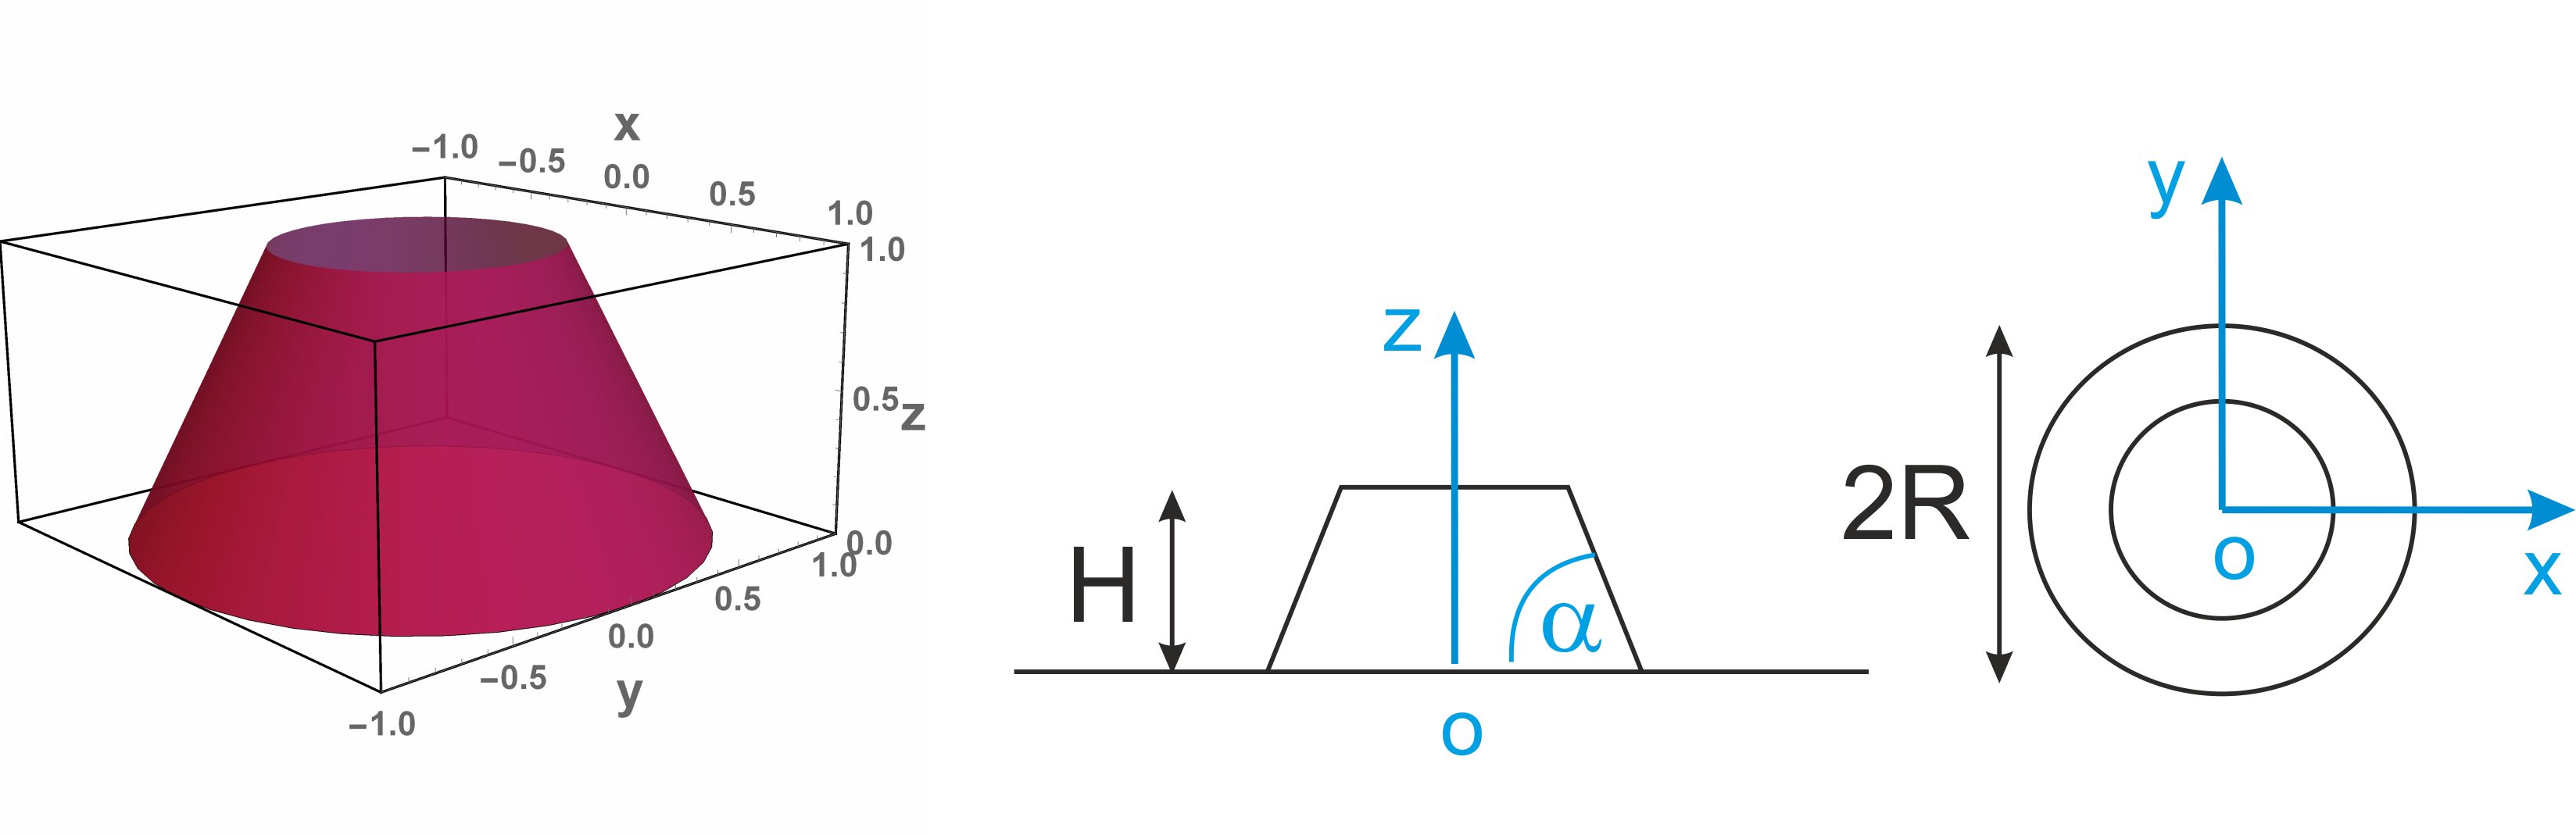
\includegraphics[width=0.9\textwidth]{../images/form_factor/oriented_primitive_opbjects/cone.png}
\end{center}
\caption{unit cone of radius $R=1$, height $H_R$ and  tilting angle $\alpha_\mathrm{tilt}$.}
\label{fig:opo_cone}
\end{figure}

The basic formula for the form factor of a  blunted cone has been taken from \cite{Renaud2009}. The difference to that version is that the affine transformation from above is used to scale the size of the cone. This is also the reason why the ratio of the height and radius $H_R=\frac{H}{R}$ is used as an input parameter instead of $H$ and $R$ separately, i.e.\ a unit cone is assumed to have a radius of $R=1$. The overall size is then scaled with the input parameters $a$, $b$ and $c$. The shape does not has inversion symmetry and is therefore a complex function. The phase factor is taken so that the base plane lies in the $xy$-plane according to fig.\ \ref{fig:opo_cone}. The form factor of the cone according to \cite{Renaud2009} is given as
\begin{align}\label{eq:opo_cone}
  F_\mathrm{cone}(\mathbf{Q},R,H,\alpha_\mathrm{tilt}) & = \int_0^H2\pi R_z^2 \frac{J_1\left(q_\parallel R_z\right)}{q_\parallel R_z}  e^{\imath \tilde{Q}_z z} \mathrm{d}z\\
  q_\parallel &= \sqrt{\tilde{Q}_x^2+\tilde{Q}_y^2} \\
  R_z &=R-z\cot(\alpha_\mathrm{tilt}) \\
  \frac{H}{R} &< \tan(\alpha_\mathrm{tilt})
\end{align}
For a random oriented oblique cone the orientation average is done over all directions of $\B{Q}$. The corresponding scattering amplitude $F_{\mathrm{cone},rnd}$ and scattering intensity $P_{\mathrm{cone},rnd}$ are then given by
\begin{align}
F_{\mathrm{cone,rnd}}(Q) &= \left\langle F_\mathrm{cone}(\B{Q})\right\rangle_\B{Q} = \int_0^\pi\mathrm{d}\theta \int_0^{2\pi}\mathrm{d}\phi \; F_\mathrm{cone}\left(Q\begin{pmatrix}
                                       \cos(\phi)\sin(\theta) \\
                                       \sin(\phi)\sin(\theta) \\
                                       \cos(\theta)
                                     \end{pmatrix}\right) \\
P_{\mathrm{cone,rnd}}(Q) &= \left\langle F_\mathrm{cone}^2(\B{Q})\right\rangle_\B{Q} = \int_0^\pi\mathrm{d}\theta \int_0^{2\pi}\mathrm{d}\phi \; F_\mathrm{cone}^2\left(Q\begin{pmatrix}
                                       \cos(\phi)\sin(\theta) \\
                                       \sin(\phi)\sin(\theta) \\
                                       \cos(\theta)
                                     \end{pmatrix}\right)
\end{align}

\begin{figure}[htb]
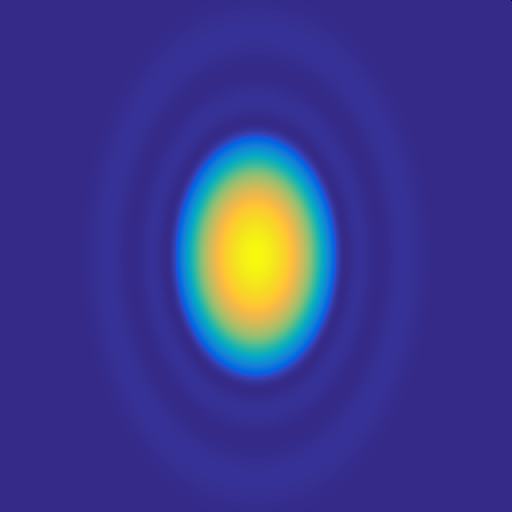
\includegraphics[width=0.31\textwidth]{../images/form_factor/oriented_primitive_opbjects/cone_0_0_0_18m.png} \hfill
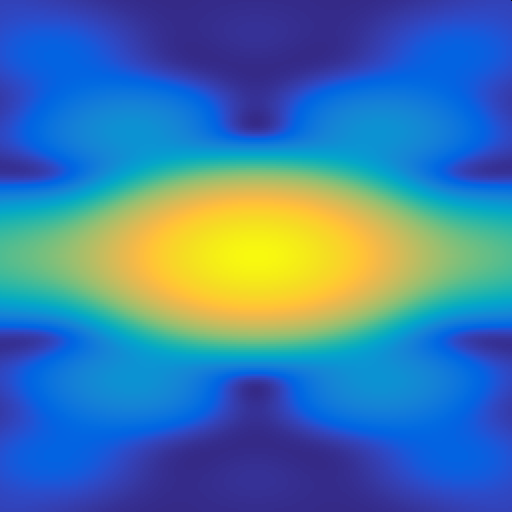
\includegraphics[width=0.31\textwidth]{../images/form_factor/oriented_primitive_opbjects/cone_0_90_0_18m.png}  \hfill 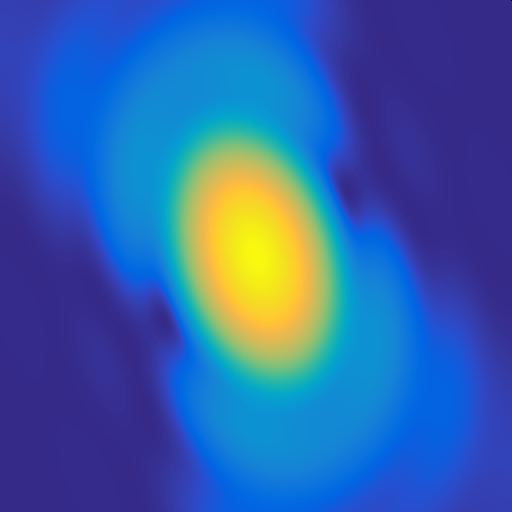
\includegraphics[width=0.31\textwidth]{../images/form_factor/oriented_primitive_opbjects/cone_0_45_45_18m.png}
\caption{Scattering patterns at 18m detector distance and a wavelength of $\lambda=0.6$nm. The cones are simulated with half axis length of $a=30$nm, $b=20$nm, and $c=10$nm and $\alpha_\mathrm{tilt}=\arctan(2)$ and $H_R=2$. The Tait–Bryan angles (yaw-pitch-roll) are $(\alpha=0^\circ,\beta=0^\circ,\gamma=0^\circ)$, $(\alpha=0^\circ,\beta=90^\circ,\gamma=0^\circ)$, and $(\alpha=0^\circ,\beta=45^\circ,\gamma=45^\circ)$ }
\label{fig:opo_coneIQ2D}
\end{figure}

~\\
\uline{Input Parameters for model \texttt{cone (opo)}:}
\begin{description}
\item[\texttt{a}] length of first half axis
\item[\texttt{ea\_x}] $x$-component of fist axis.
\item[\texttt{ea\_y}] $y$-component of fist axis.
\item[\texttt{ea\_z}] $z$-component of fist axis.
\item[\texttt{b}] length of second half axis
\item[\texttt{eb\_x}] $x$-component of second axis.
\item[\texttt{eb\_y}] $y$-component of second axis.
\item[\texttt{eb\_z}] $z$-component of second axis.
\item[\texttt{c}] length of third axis
\item[\texttt{ec\_x}] $x$-component of third axis.
\item[\texttt{ec\_y}] $y$-component of third axis.
\item[\texttt{ec\_z}] $z$-component of third axis.
\item[\texttt{eta\_p}] scattering length density $\eta_p$ of particle
\item[\texttt{eta\_m}] scattering length density $\eta_m$ of matrix
\item[\texttt{alpha}] first Euler angle
\item[\texttt{beta}] second Euler angle
\item[\texttt{gamma}] third Euler angle
\item[\texttt{psi}] direction of $\B{Q}$ on detector ($\psi=0$, $x$-direction, to the right)
\item[\texttt{tilt}] tilt angle $\alpha_\mathrm{tilt}$ of conical side wall of unit cone
\item[\texttt{H\_R}] height of unit cone $H_R$
\end{description}

\begin{figure}[htb]
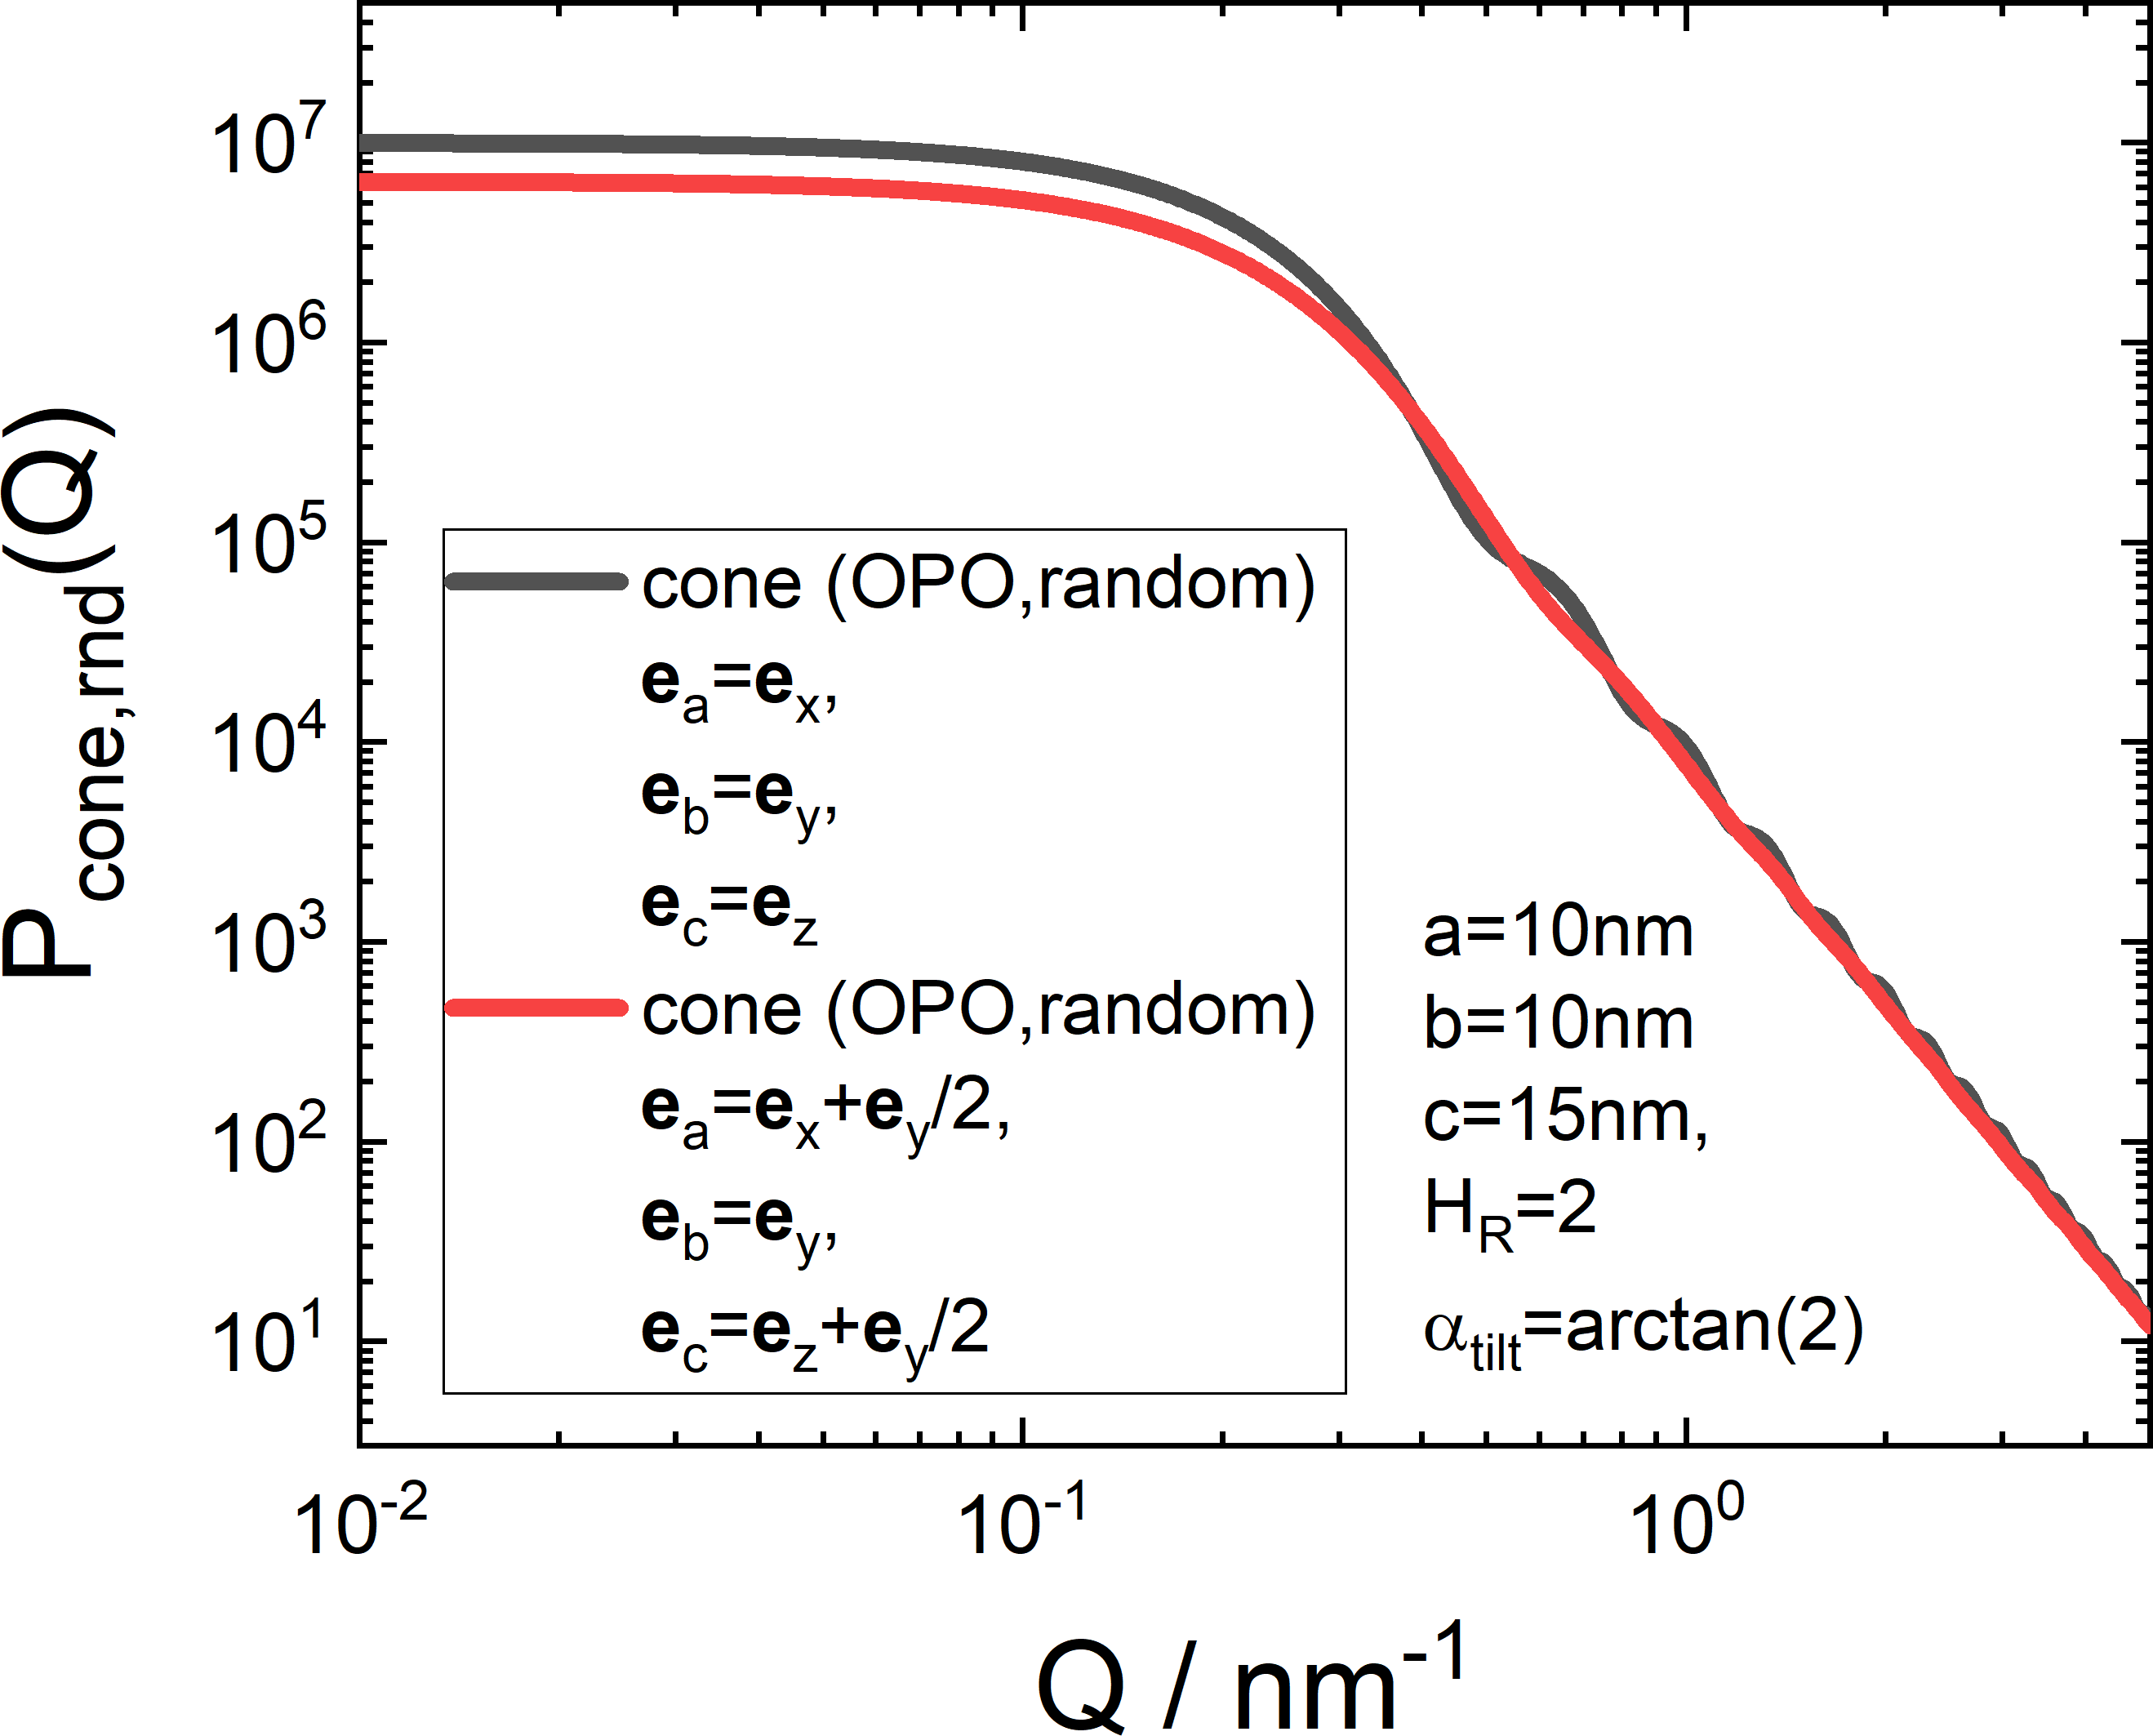
\includegraphics[width=0.481\textwidth]{../images/form_factor/oriented_primitive_opbjects/coneOPOoblique.png} \hfill
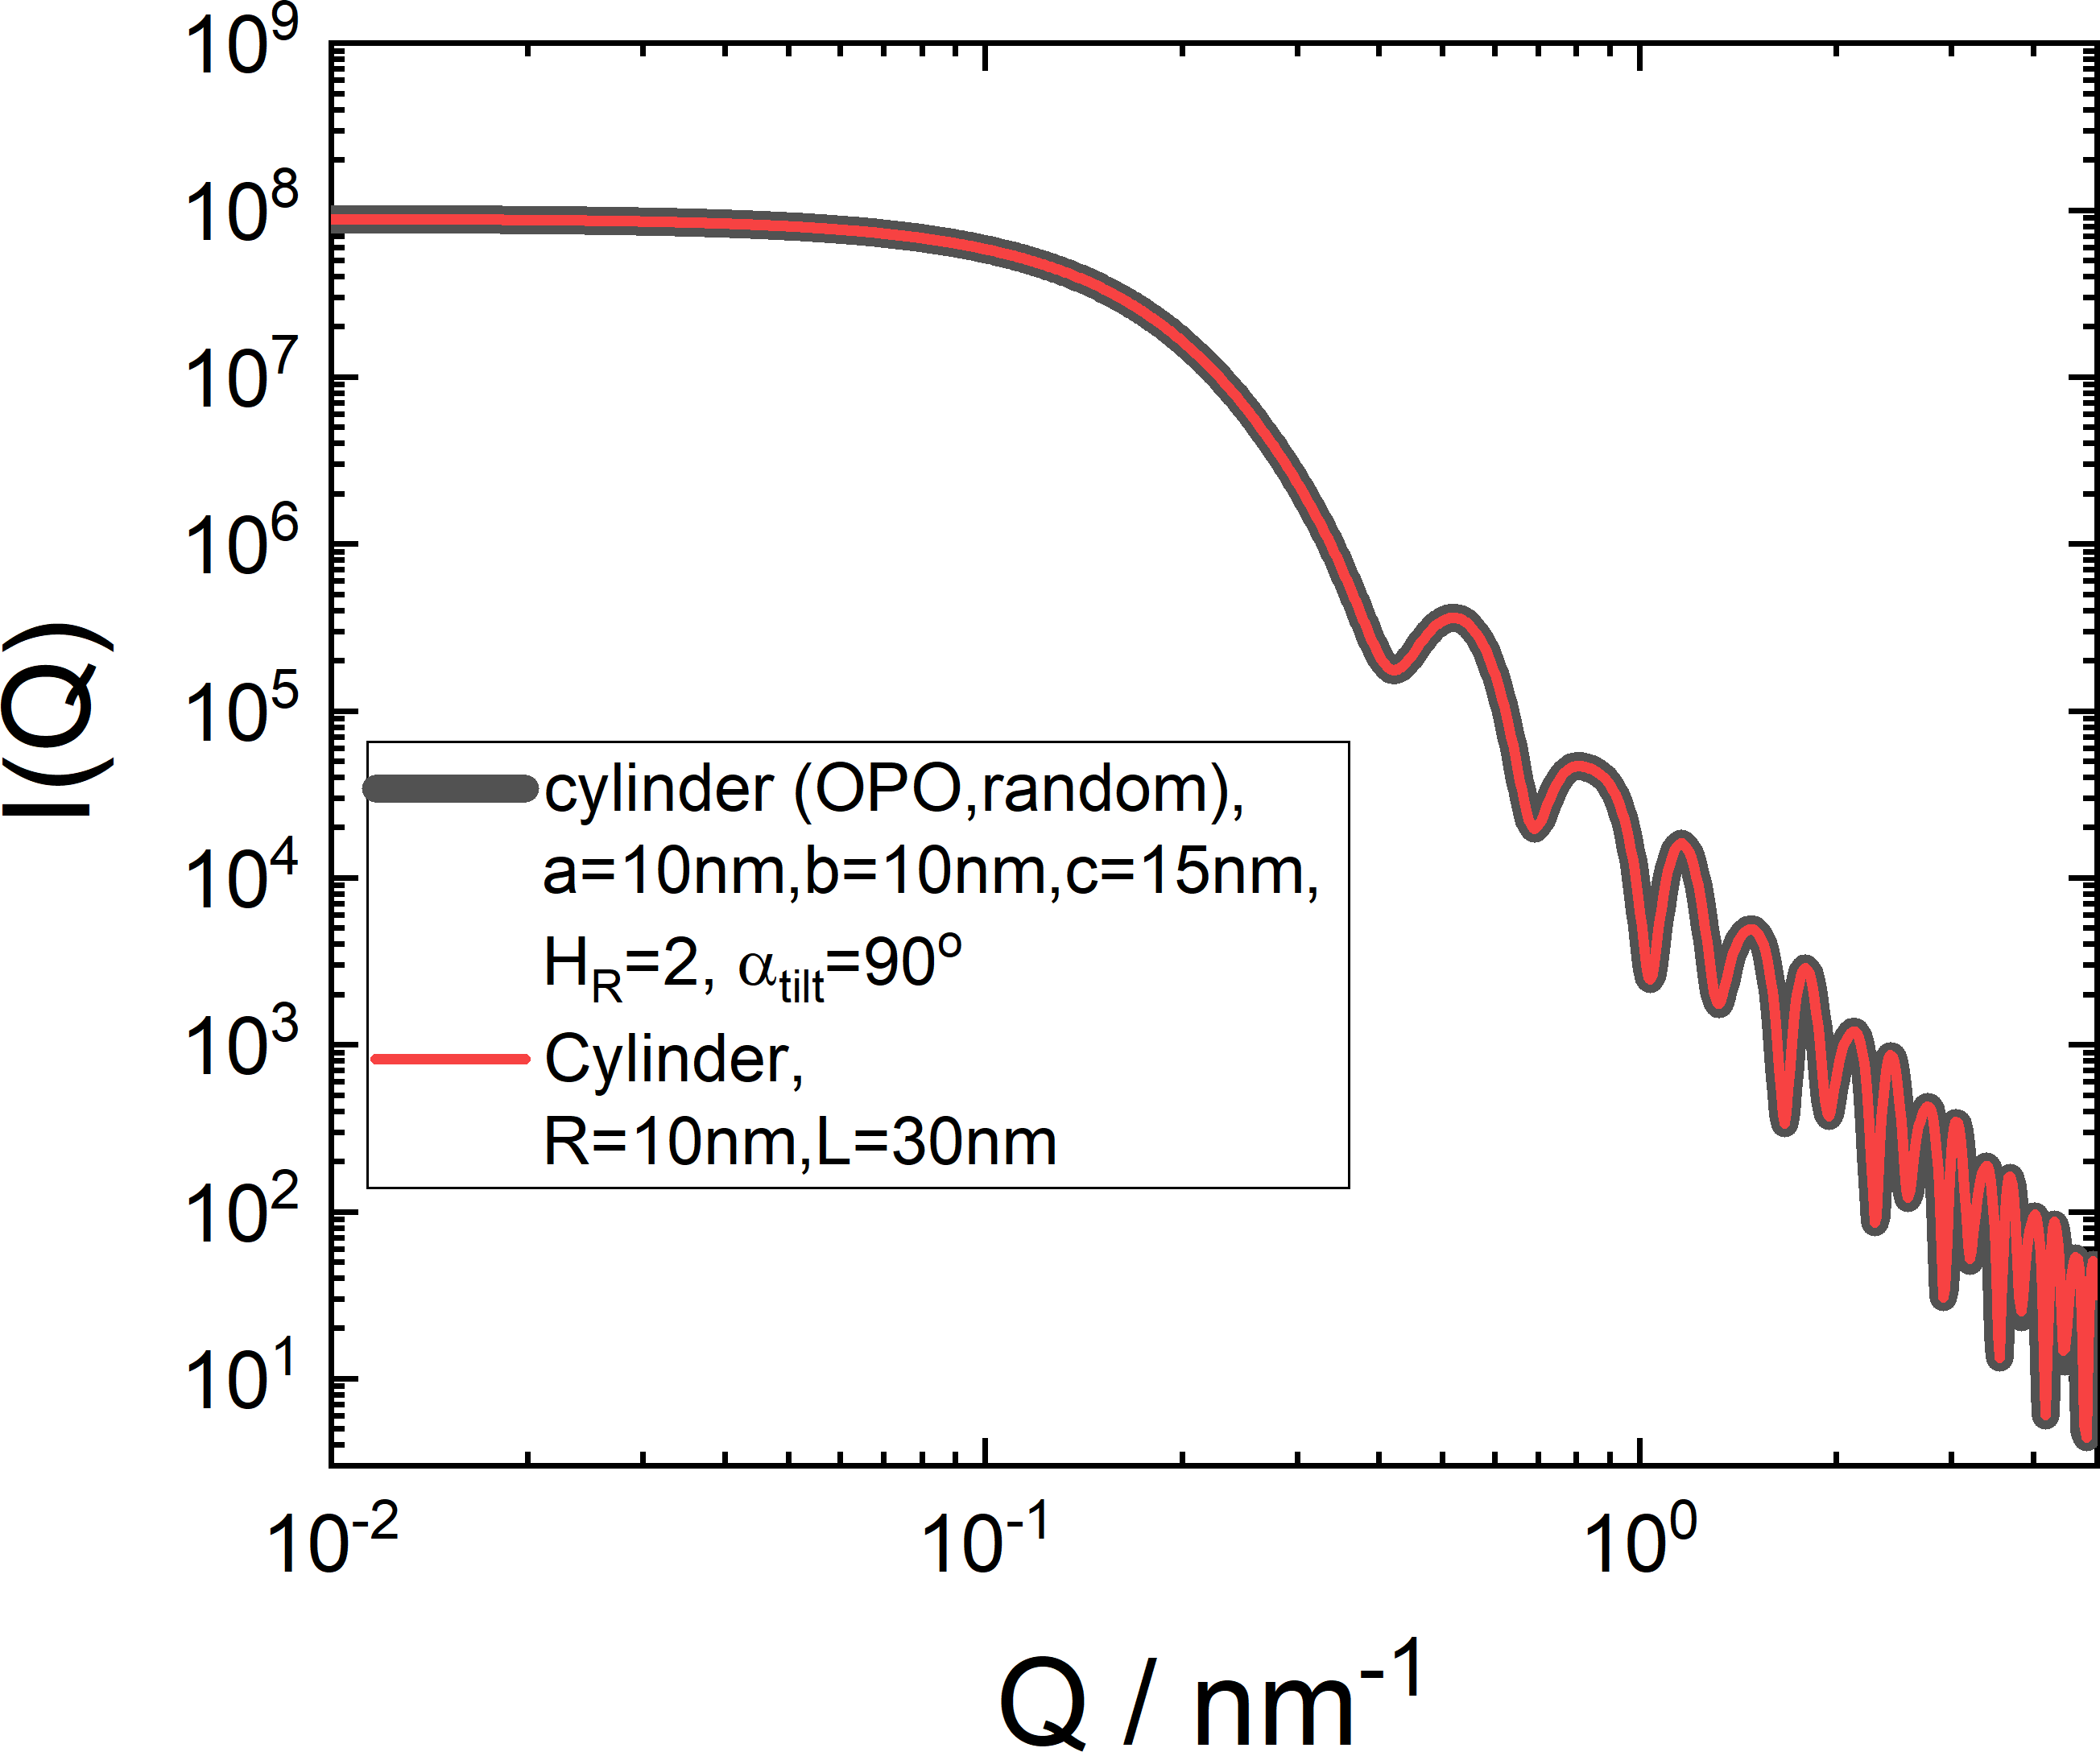
\includegraphics[width=0.481\textwidth]{../images/form_factor/oriented_primitive_opbjects/coneOPOcompare.png}
\caption{scattering curved of an oblique \texttt{cone (OPO,random)} (left) and a comparison of a \texttt{cone (OPO,random)} with a random oriented solid cylinder \texttt{Cylinder} form factor (right)}
\label{fig:opo_coneIQrandom}
\end{figure}

~\\
\uline{Input Parameters for model \texttt{cone (opo, random)}:}
\begin{description}
\item[\texttt{a}] length of first half axis
\item[\texttt{ea\_x}] $x$-component of fist axis.
\item[\texttt{ea\_y}] $y$-component of fist axis.
\item[\texttt{ea\_z}] $z$-component of fist axis.
\item[\texttt{b}] length of second half axis
\item[\texttt{eb\_x}] $x$-component of second axis.
\item[\texttt{eb\_y}] $y$-component of second axis.
\item[\texttt{eb\_z}] $z$-component of second axis.
\item[\texttt{c}] length of third axis
\item[\texttt{ec\_x}] $x$-component of third axis.
\item[\texttt{ec\_y}] $y$-component of third axis.
\item[\texttt{ec\_z}] $z$-component of third axis.
\item[\texttt{eta\_p}] scattering length density $\eta_p$ of particle
\item[\texttt{eta\_m}] scattering length density $\eta_m$ of matrix
\item[\texttt{dummy}] not used
\item[\texttt{dummy}] not used
\item[\texttt{dummy}] not used
\item[\texttt{dummy}] not used
\item[\texttt{tilt}] tilt angle $\alpha_\mathrm{tilt}$ of conical side wall of unit cone
\item[\texttt{H\_R}] height of unit cone $H_R$
\end{description}

\noindent\uline{Note:}
\begin{itemize}
\item the unit vector $\B{e}_a$, $\B{e}_b$, and $\B{e}_c$ are internally normalized to 1 and need to be linear independent.
\item $a$ and $b$ are the half axis or radii of the elliptical base and $cH_R$ the full height of the cone.
\item the volume of the oblique cone is $$V_\mathrm{cone}=\frac{\pi}{3}\tan(\alpha_\mathrm{tilt})\left[1-\left(1-\frac{H_\mathrm{R}}{\tan(\alpha_\mathrm{tilt})}\right)^3\right] \det(\M{D}^{-1})$$
\end{itemize}

\subsection{oriented and random oriented cone with 6-fold symmetry} ~\\

\begin{figure}[htb]
\begin{center}
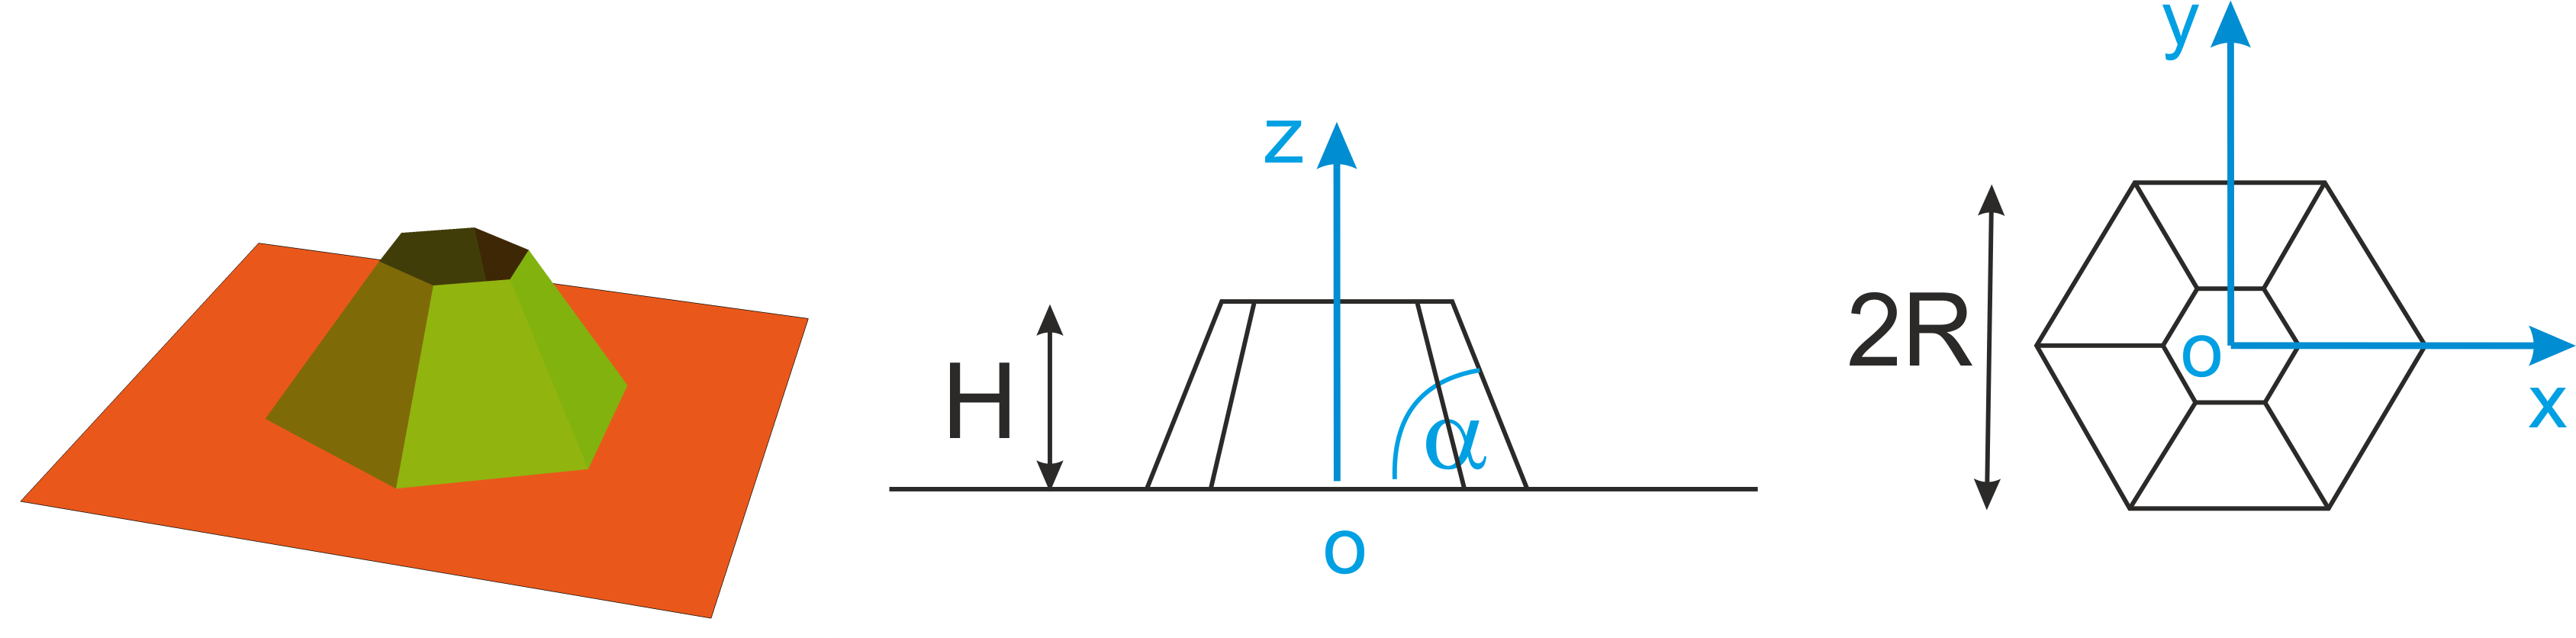
\includegraphics[width=0.95\textwidth]{../images/form_factor/oriented_primitive_opbjects/cone6.png}
\end{center}
\caption{unit cone with 6-fold symmetry (blunted hexagonal pyramid), diameter of $2R=2$, height $H_R$ and tilting angle $\alpha_\mathrm{tilt}$.}
\label{fig:opo_cone6}
\end{figure}

The basic formula for the form factor of a cone with a 6-fold symmetry (blunted hexagonal pyramid) has been taken from \cite{Renaud2009}. The difference to that version is that the affine transformation from above is used to scale the size of the cone. This is also the reason why the ratio of the height and radius $H_R=\frac{H}{R}$ is used as an input parameter instead of $H$ and $R$ separately, i.e.\ a unit 6-fold symmetric cone is assumed to have a radius of $R=1$. The overall size is then scaled with the input parameters $a$, $b$ and $c$. The shape does not has inversion symmetry and is therefore a complex function. The phase factor is taken so that the base plane lies in the $xy$-plane according to fig.\ \ref{fig:opo_cone6}. The form factor of the cone according to \cite{Renaud2009} is given as
\begin{align}\label{eq:opo_cone6}
\begin{split}
   F_\mathrm{cone6}(\mathbf{Q},R,H,\alpha_\mathrm{tilt})
     & = \frac{4\sqrt{3}}{3\tilde{Q}_y^2-\tilde{Q}_x^2} \int_0^H \Bigg[\tilde{Q}_y^2R_z^2  \frac{\sin\left(\tilde{Q}_x R_z/\sqrt{3}\right)}{\tilde{Q}_x R_z/\sqrt{3}} \frac{\sin(\tilde{Q}_y R_z)}{\tilde{Q}_y R_z} \\
     &  + \cos\left(2\tilde{Q}_x R_z/\sqrt{3}\right) -\cos(\tilde{Q}_y R_z)\cos\left(\tilde{Q}_x R_z/\sqrt{3}\right) \Bigg] \\
     & \times e^{\imath \tilde{Q}_z z} \mathrm{d}z
\end{split} \\
  R_z &=R-z\cot(\alpha_\mathrm{tilt}) \\
  \frac{H}{R} &< \tan(\alpha_\mathrm{tilt})
\end{align}

\begin{figure}[htb]
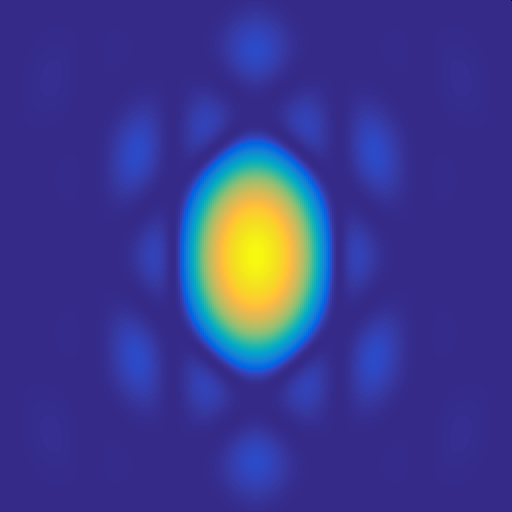
\includegraphics[width=0.31\textwidth]{../images/form_factor/oriented_primitive_opbjects/cone6_0_0_0_18m.png} \hfill
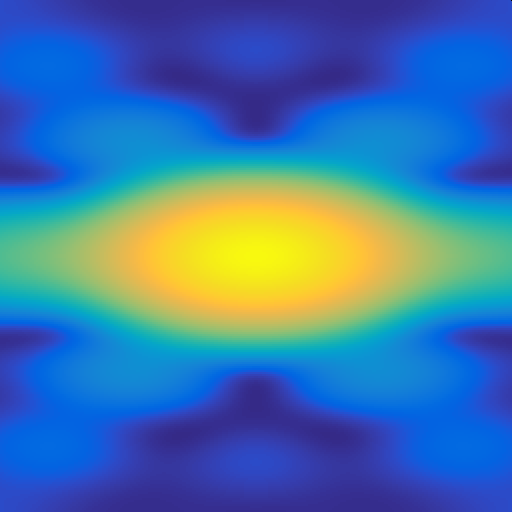
\includegraphics[width=0.31\textwidth]{../images/form_factor/oriented_primitive_opbjects/cone6_0_90_0_18m.png}  \hfill 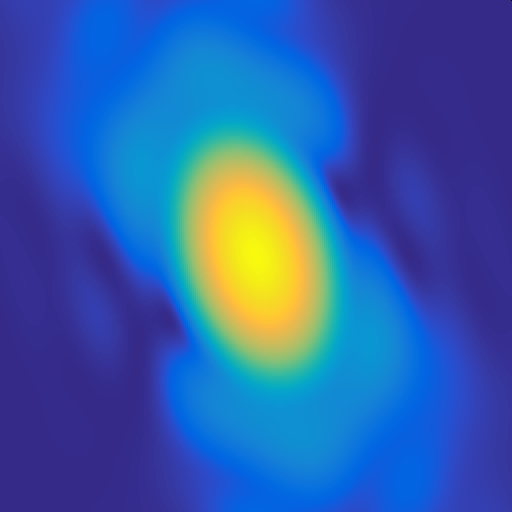
\includegraphics[width=0.31\textwidth]{../images/form_factor/oriented_primitive_opbjects/cone6_0_45_45_18m.png}
\caption{Scattering patterns at 18m detector distance and a wavelength of $\lambda=0.6$nm. The cones with 6-fold symmetry are simulated with half axis length of $a=30$nm, $b=20$nm, and $c=10$nm and $\alpha_\mathrm{tilt}=\arctan(2)$ and $H_R=2$. The Tait–Bryan angles (yaw-pitch-roll) are $(\alpha=0^\circ,\beta=0^\circ,\gamma=0^\circ)$, $(\alpha=0^\circ,\beta=90^\circ,\gamma=0^\circ)$, and $(\alpha=0^\circ,\beta=45^\circ,\gamma=45^\circ)$ }
\label{fig:opo_coneIQ2D}
\end{figure}

~\\
\uline{Input Parameters for model \texttt{cone6 (opo)}:}
\begin{description}
\item[\texttt{a}] length of first half axis
\item[\texttt{ea\_x}] $x$-component of fist axis.
\item[\texttt{ea\_y}] $y$-component of fist axis.
\item[\texttt{ea\_z}] $z$-component of fist axis.
\item[\texttt{b}] length of second half axis
\item[\texttt{eb\_x}] $x$-component of second axis.
\item[\texttt{eb\_y}] $y$-component of second axis.
\item[\texttt{eb\_z}] $z$-component of second axis.
\item[\texttt{c}] length of third axis
\item[\texttt{ec\_x}] $x$-component of third axis.
\item[\texttt{ec\_y}] $y$-component of third axis.
\item[\texttt{ec\_z}] $z$-component of third axis.
\item[\texttt{eta\_p}] scattering length density $\eta_p$ of particle
\item[\texttt{eta\_m}] scattering length density $\eta_m$ of matrix
\item[\texttt{alpha}] first Euler angle
\item[\texttt{beta}] second Euler angle
\item[\texttt{gamma}] third Euler angle
\item[\texttt{psi}] direction of $\B{Q}$ on detector ($\psi=0$, $x$-direction, to the right)
\item[\texttt{tilt}] tilt angle $\alpha_\mathrm{tilt}$ of conical side wall of unit cone
\item[\texttt{H\_R}] height $H_R$ of unit 6-fold symmetric cone
\end{description}

\begin{figure}[htb]
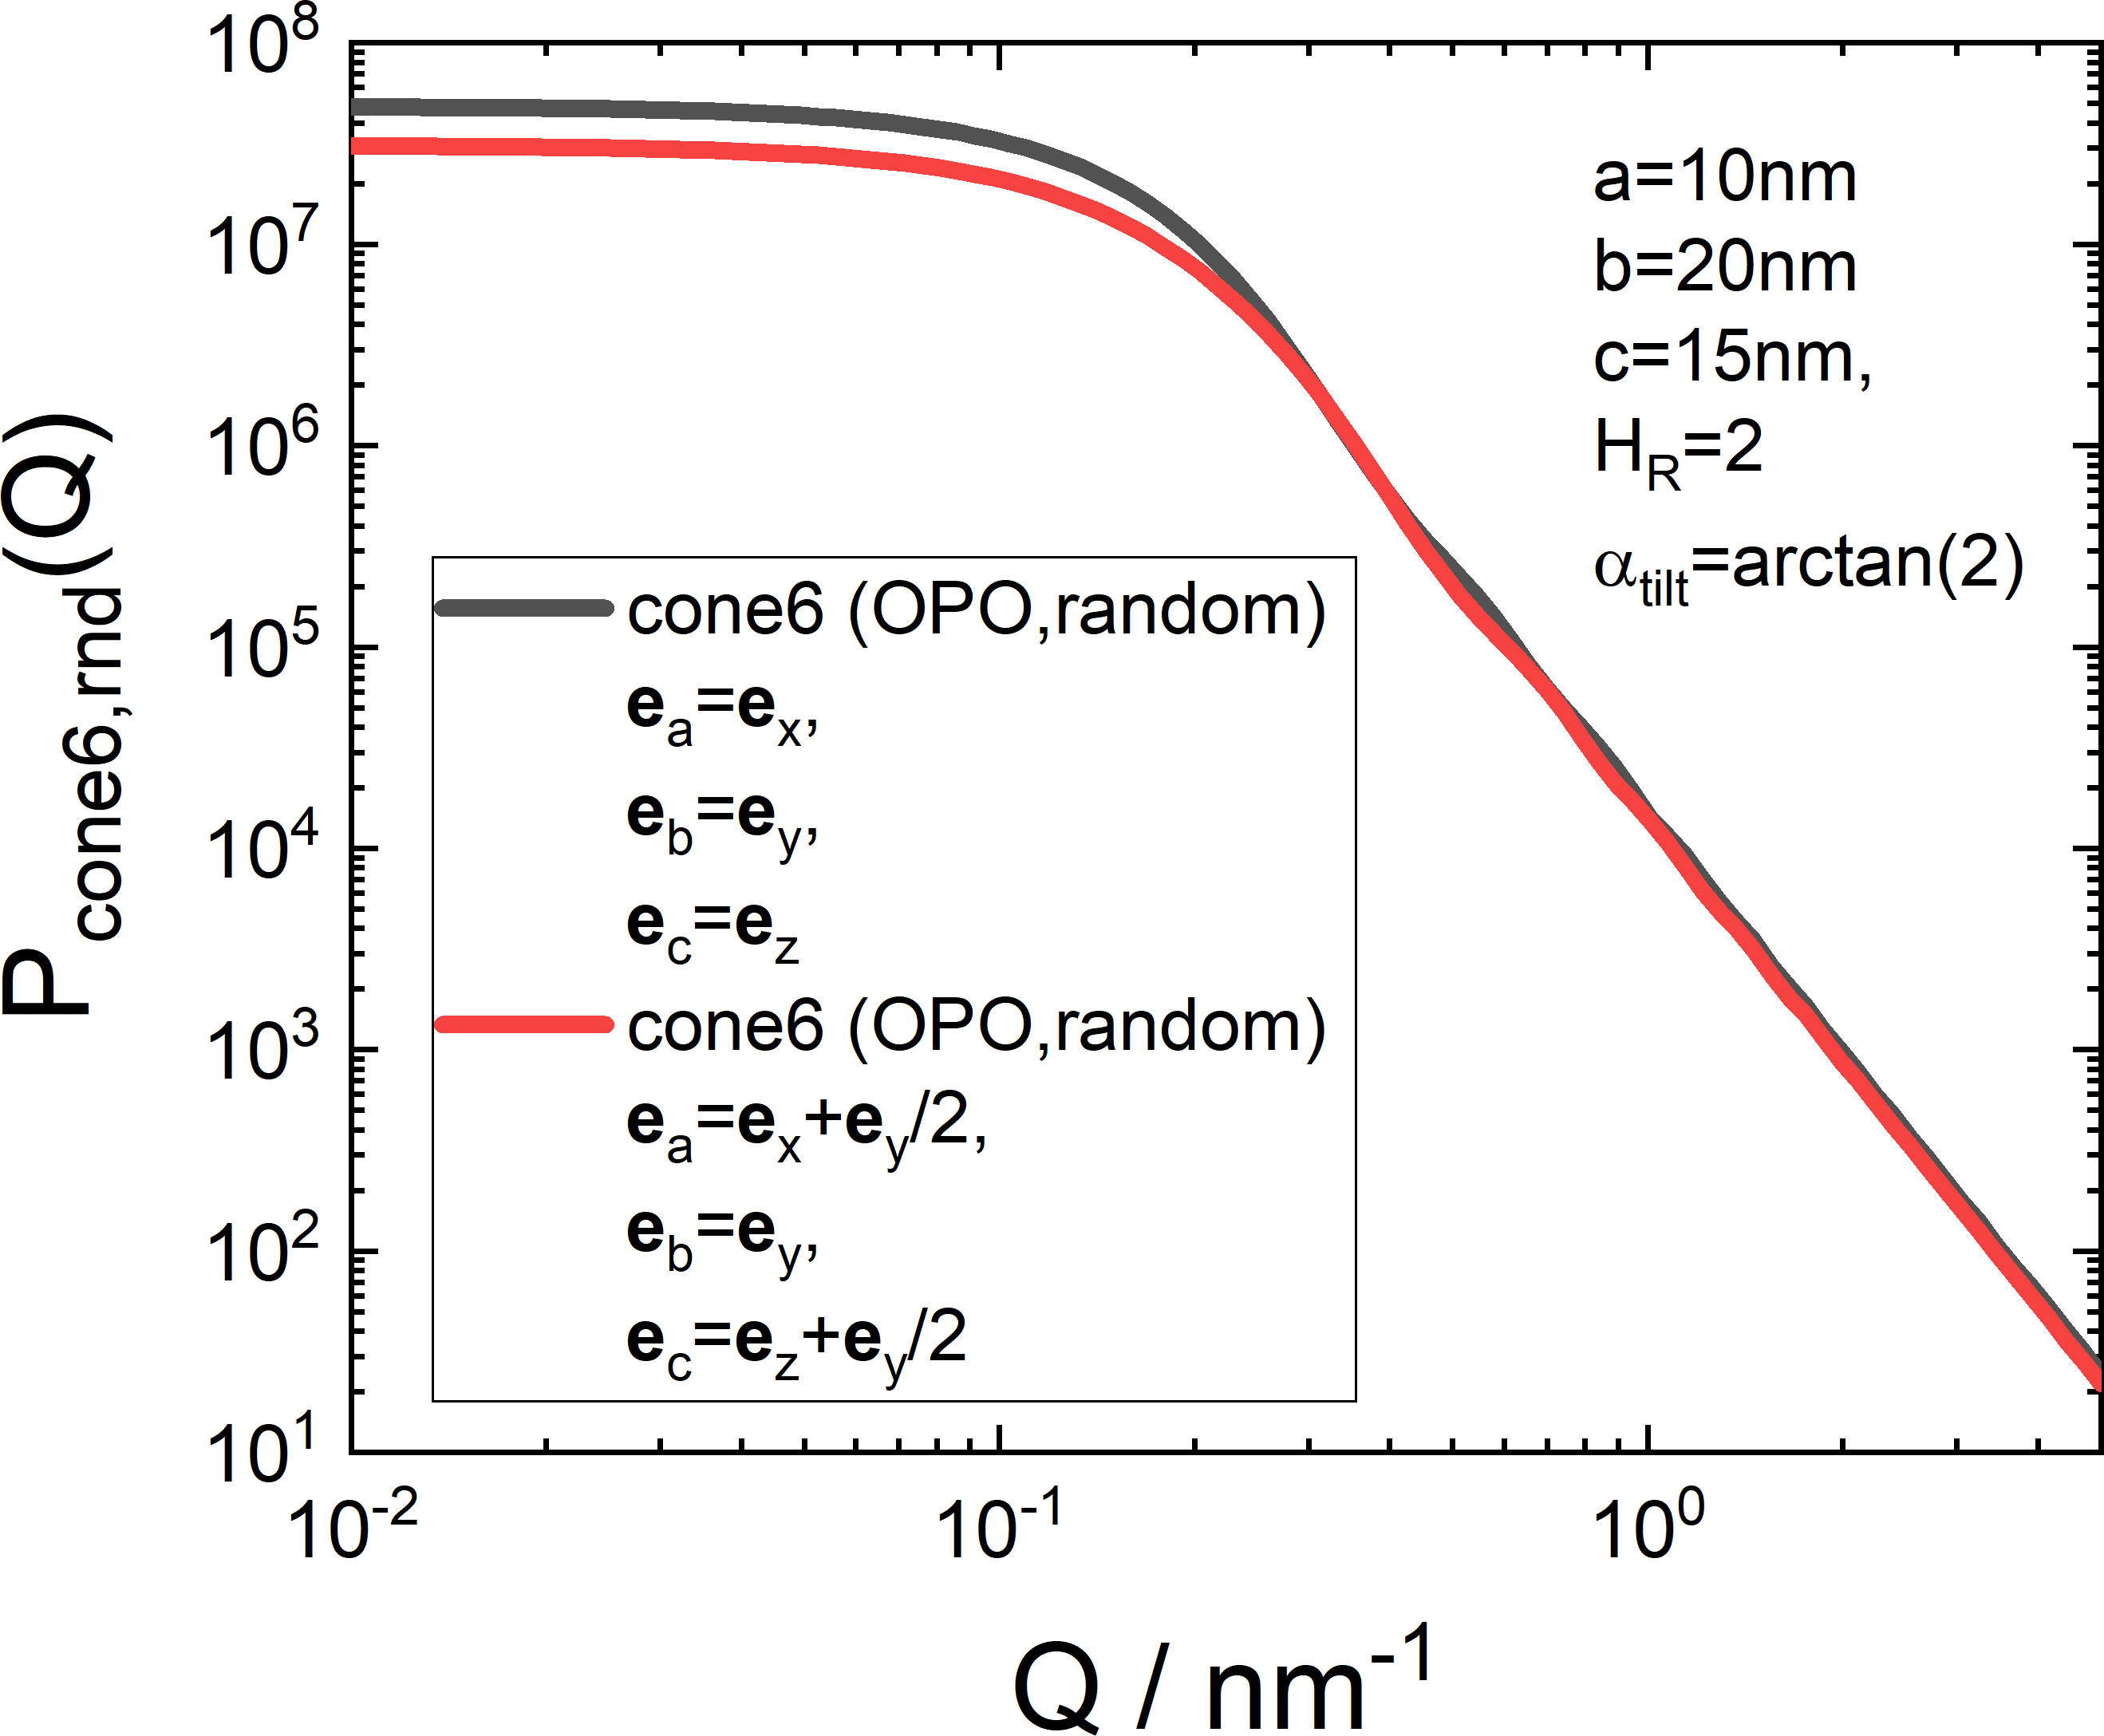
\includegraphics[width=0.481\textwidth]{../images/form_factor/oriented_primitive_opbjects/cone6OPOoblique.png} \hfill
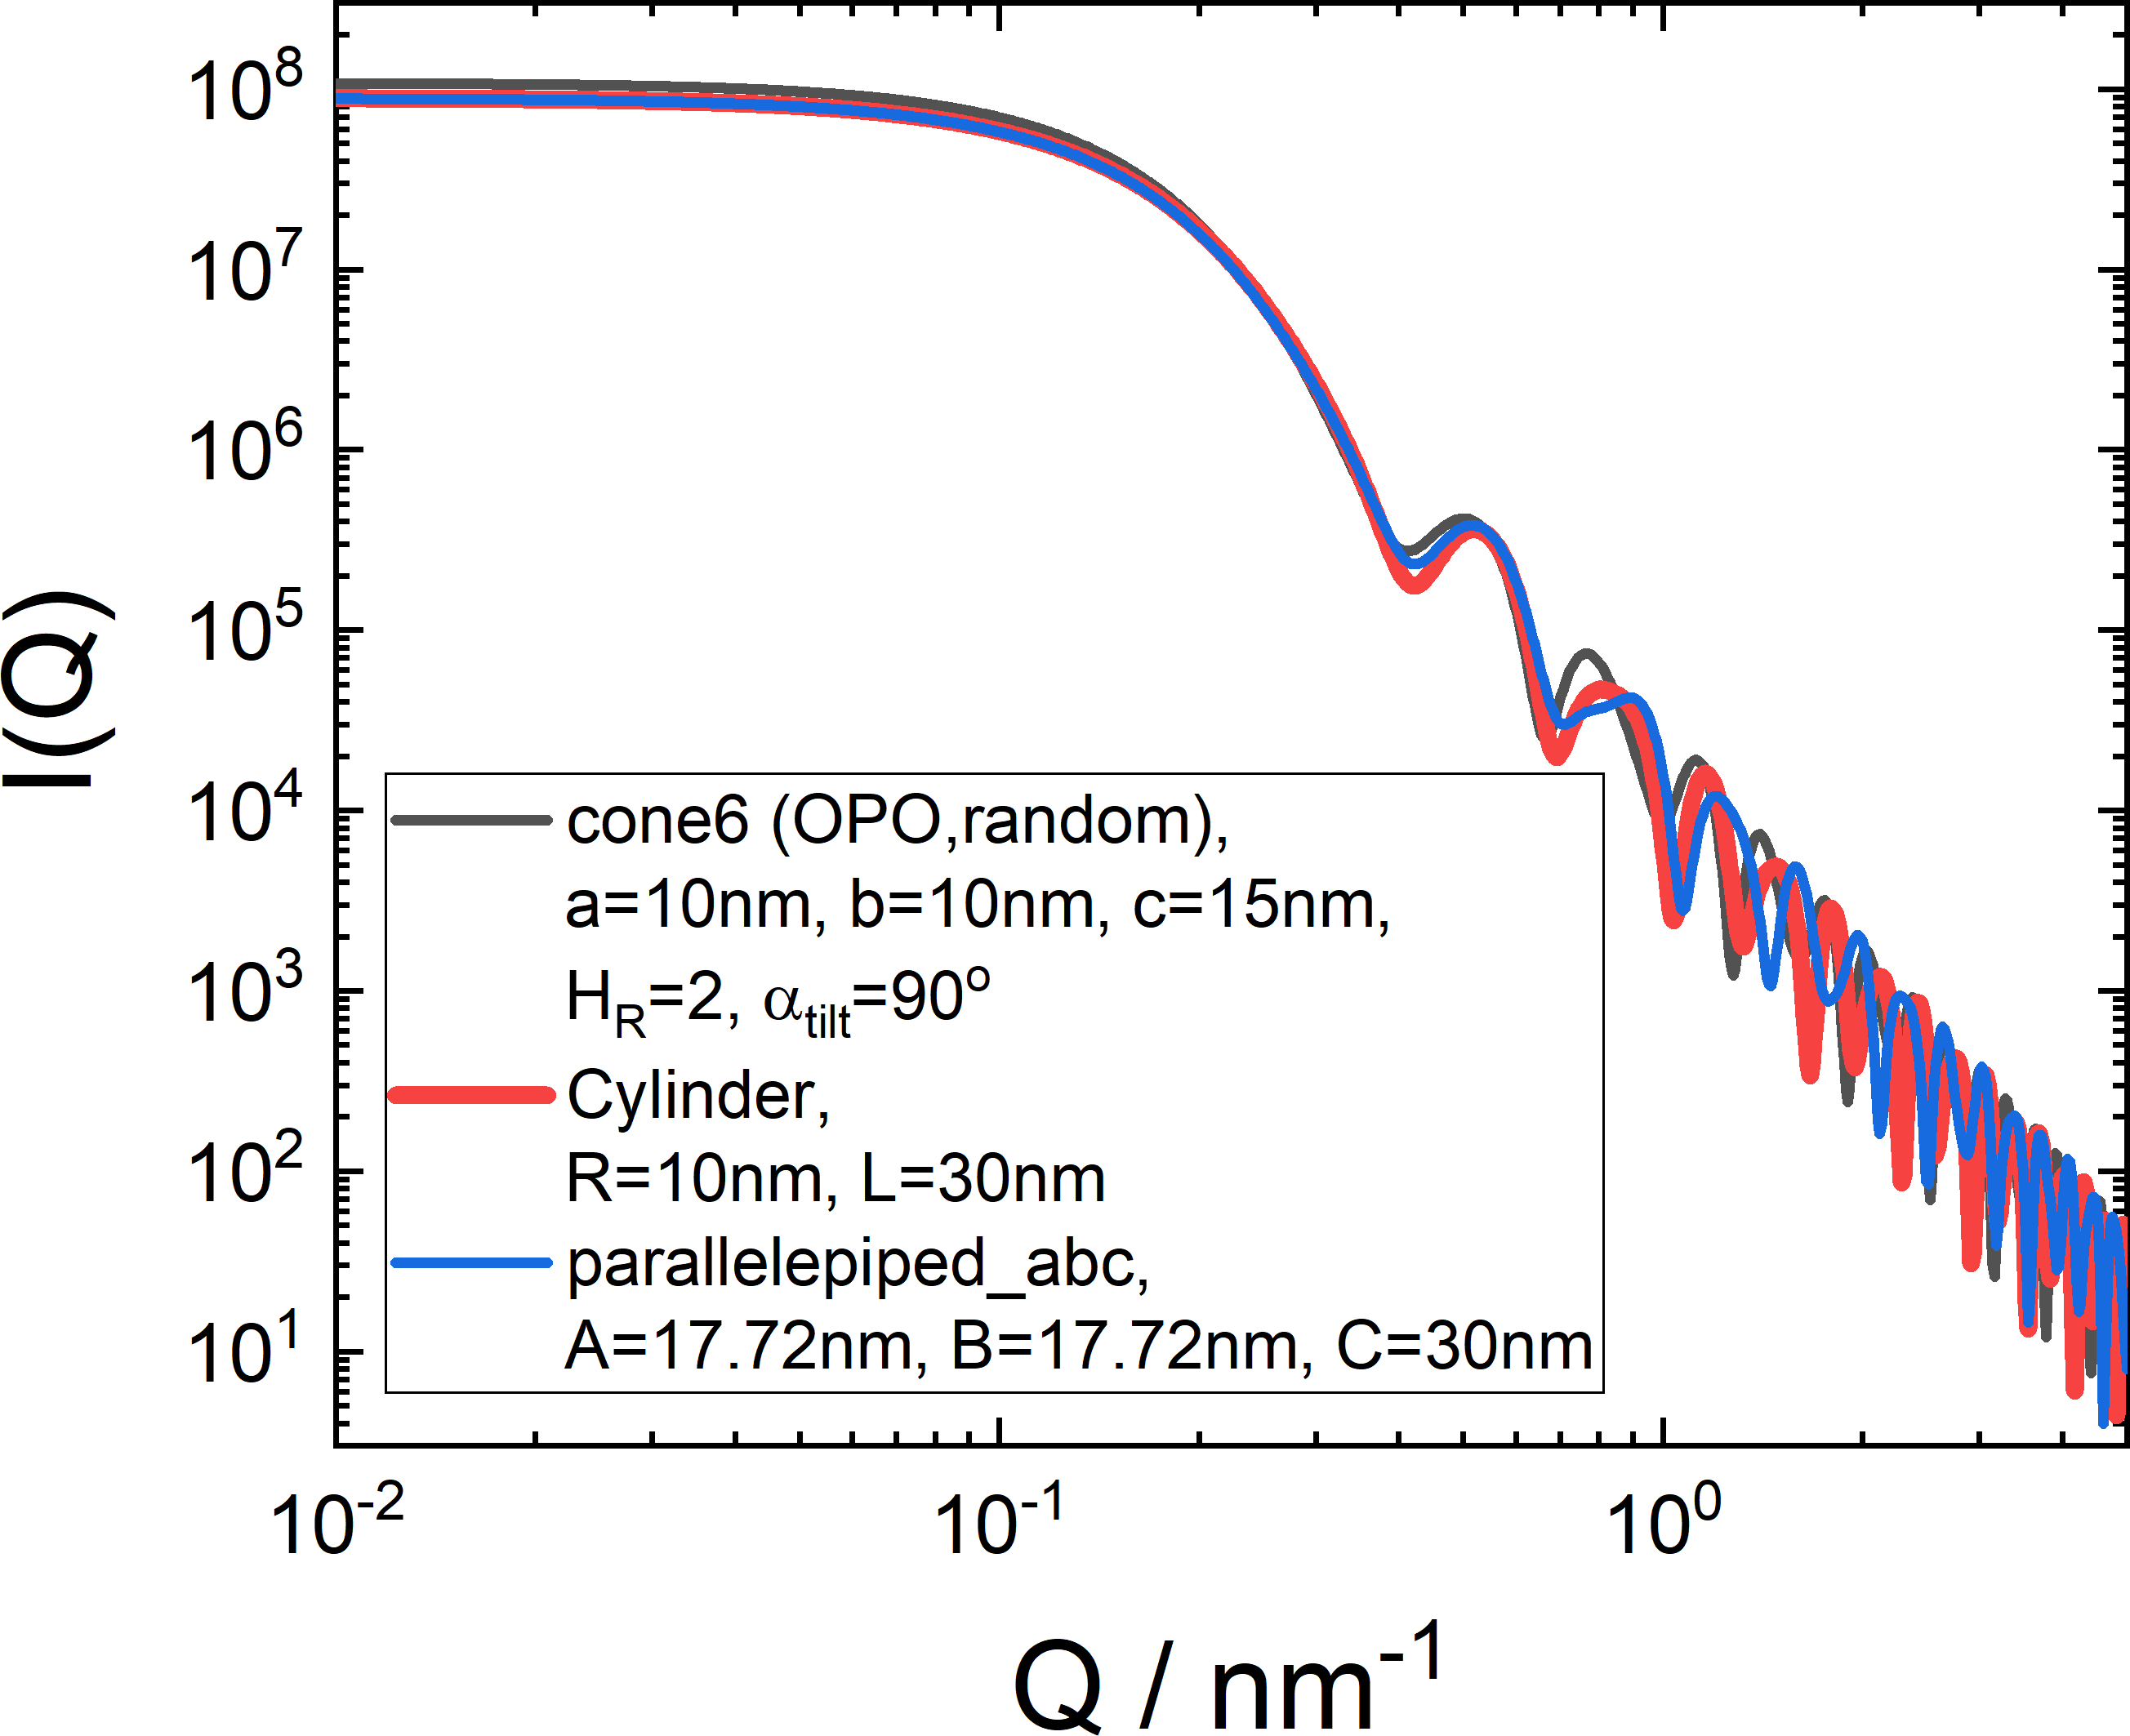
\includegraphics[width=0.481\textwidth]{../images/form_factor/oriented_primitive_opbjects/cone6OPOcompare.png}
\caption{scattering curved of an oblique \texttt{cone6 (OPO,random)} (left) and a comparison of a \texttt{cone6 (OPO,random)} with a random oriented solid cylinder \texttt{Cylinder} form factor and a random oriented parallelepiped \texttt{parallelepiped\_abc} (right)}
\label{fig:opo_cone6IQrandom}
\end{figure}

~\\
\uline{Input Parameters for model \texttt{cone6 (opo, random)}:}
\begin{description}
\item[\texttt{a}] length of first half axis
\item[\texttt{ea\_x}] $x$-component of fist axis.
\item[\texttt{ea\_y}] $y$-component of fist axis.
\item[\texttt{ea\_z}] $z$-component of fist axis.
\item[\texttt{b}] length of second half axis
\item[\texttt{eb\_x}] $x$-component of second axis.
\item[\texttt{eb\_y}] $y$-component of second axis.
\item[\texttt{eb\_z}] $z$-component of second axis.
\item[\texttt{c}] length of third half axis
\item[\texttt{ec\_x}] $x$-component of third axis.
\item[\texttt{ec\_y}] $y$-component of third axis.
\item[\texttt{ec\_z}] $z$-component of third axis.
\item[\texttt{eta\_p}] scattering length density $\eta_p$ of particle
\item[\texttt{eta\_m}] scattering length density $\eta_m$ of matrix
\item[\texttt{dummy}] not used
\item[\texttt{dummy}] not used
\item[\texttt{dummy}] not used
\item[\texttt{dummy}] not used
\item[\texttt{tilt}] tilt angle $\alpha_\mathrm{tilt}$ of conical side wall of unit cone
\item[\texttt{H\_R}] height $H_R$ of unit 6-fold symmetric cone
\end{description}

\noindent\uline{Note:}
\begin{itemize}
\item the unit vector $\B{e}_a$, $\B{e}_b$, and $\B{e}_c$ are internally normalized to 1 and need to be linear independent.
\item $a$ and $b$ are the half axis or radii of the elliptical base and $cH_R$ the full height of the cone.
\item the volume of the oblique 6-fold symmetric cone is $$V_\mathrm{cone}=\frac{2\tan(\alpha_\mathrm{tilt})}{\sqrt{3}}\left[1-\left(1-\frac{H_\mathrm{R}}{\tan(\alpha_\mathrm{tilt})}\right)^3\right] \det(\M{D}^{-1})$$
\end{itemize}

\subsection{oriented and random oriented tetrahedron} ~\\
\cite{Renaud2009}
\begin{figure}[htb]
\begin{center}
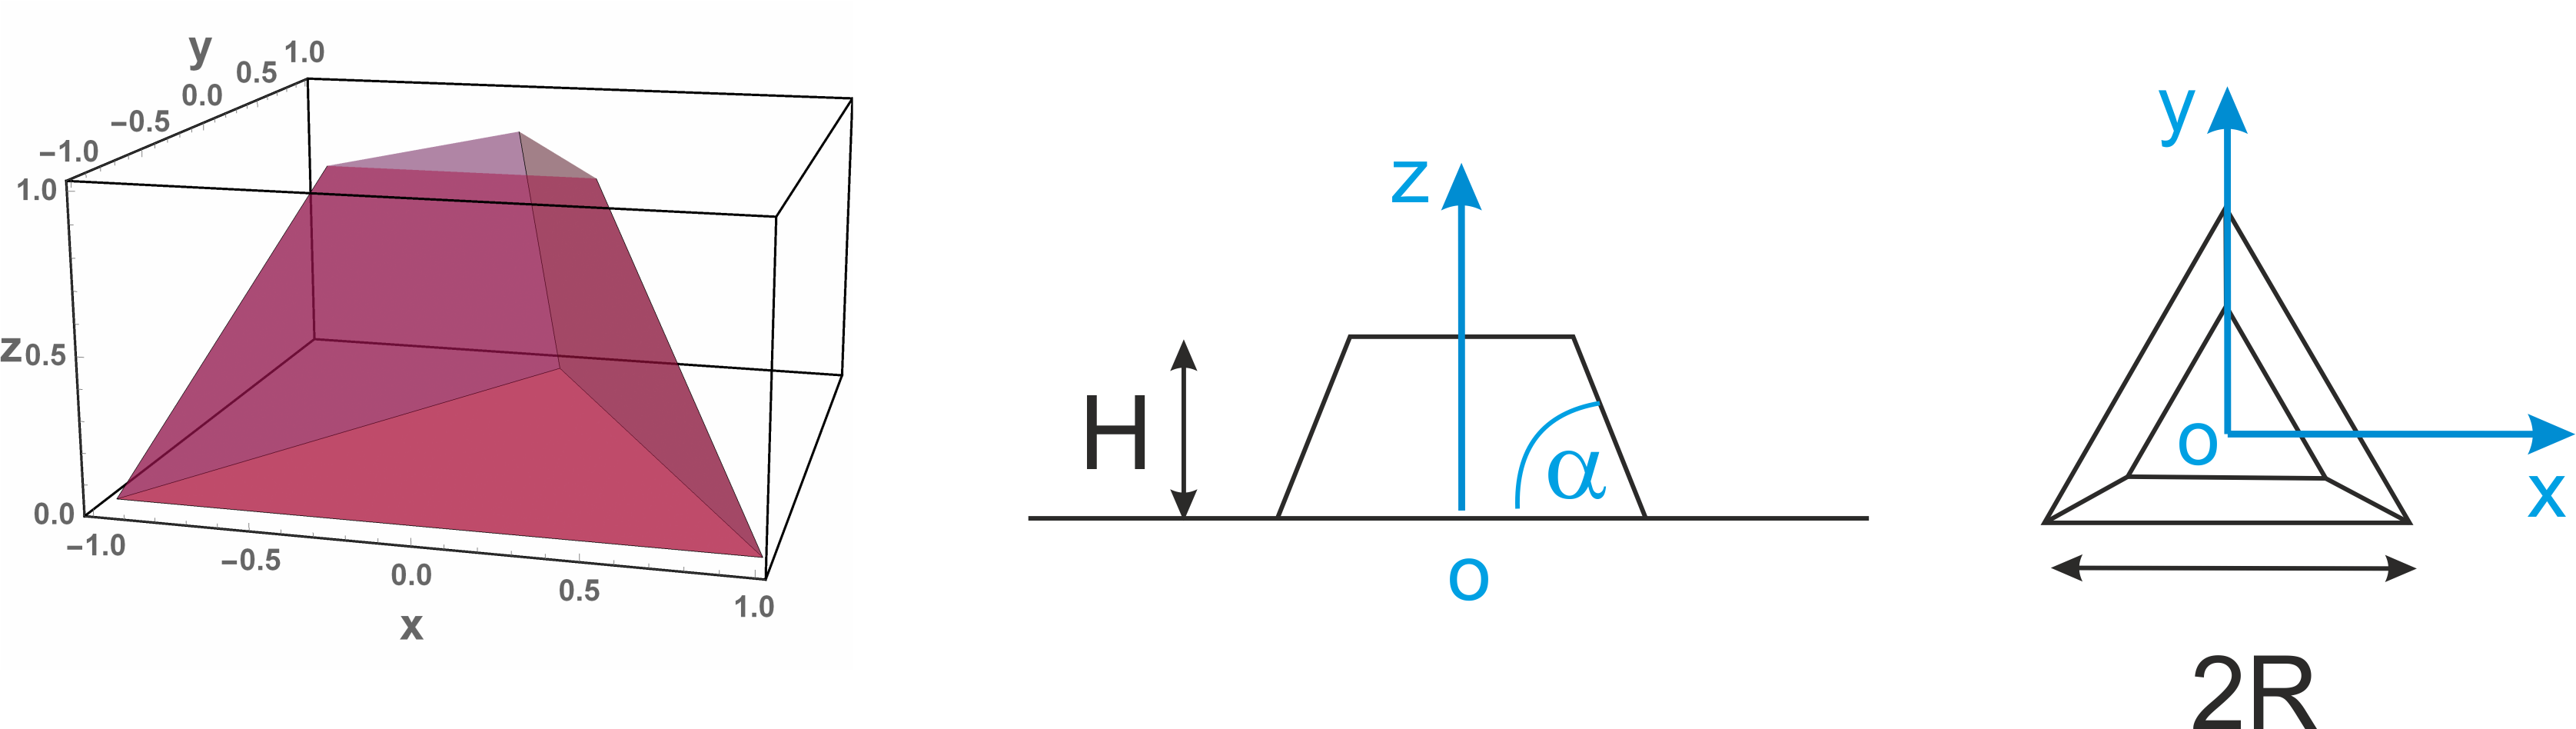
\includegraphics[width=0.9\textwidth]{../images/form_factor/oriented_primitive_opbjects/tetrahedron.png}
\end{center}
\caption{unit tetrahedron with base length of $2R=2$, height $H_R$ and tilting angle $\alpha$.}
\label{fig:opo_tetrahedron}
\end{figure}


\begin{align}\label{eq:opo_tetrah}
\begin{split}
 F_\mathrm{th}(\mathbf{Q},R,H,\alpha) & = \frac{\sqrt{3}H}{\tilde{Q}_x\left(\tilde{Q}_x^2-3\tilde{Q}_y^2\right)} e^{\imath\tilde{Q}_zR\tan(\alpha)/\sqrt{3}} \quad \times\\
     &  \Bigg\{-\left(\tilde{Q}_x+\sqrt{3}\tilde{Q}_y\right) \frac{\sin(q_1H)}{q_1H}e^{\imath q_1L}  +\\
     & \left(-\tilde{Q}_x+\sqrt{3}\tilde{Q}_y\right)\frac{\sin(q_2H)}{q_2H}e^{-\imath q_2L} +2\tilde{Q}_x \frac{\sin(q_3H)}{q_3H}e^{\imath q_3L}\Bigg\}
\end{split} \\
  q_1 & =\frac12 \left[\frac{\sqrt{3}\tilde{Q}_x-\tilde{Q}_y}{\tan(\alpha)}-\tilde{Q}_z\right]\\
  q_2 & =\frac12 \left[\frac{\sqrt{3}\tilde{Q}_x+\tilde{Q}_y}{\tan(\alpha)}+\tilde{Q}_z\right]\\
  q_3 & =\frac12 \left[\frac{2\tilde{Q}_y}{\tan(\alpha)}-\tilde{Q}_z\right]\\
  L & =\frac{2\tan(\alpha)R}{\sqrt{3}}-H\\
  \frac{H}{R} & < \frac{\tan(\alpha)}{\sqrt{3}}
\end{align}

\subsection{oriented and random oriented squared pyramid} ~\\
\cite{Renaud2009}
\begin{figure}[htb]
\begin{center}
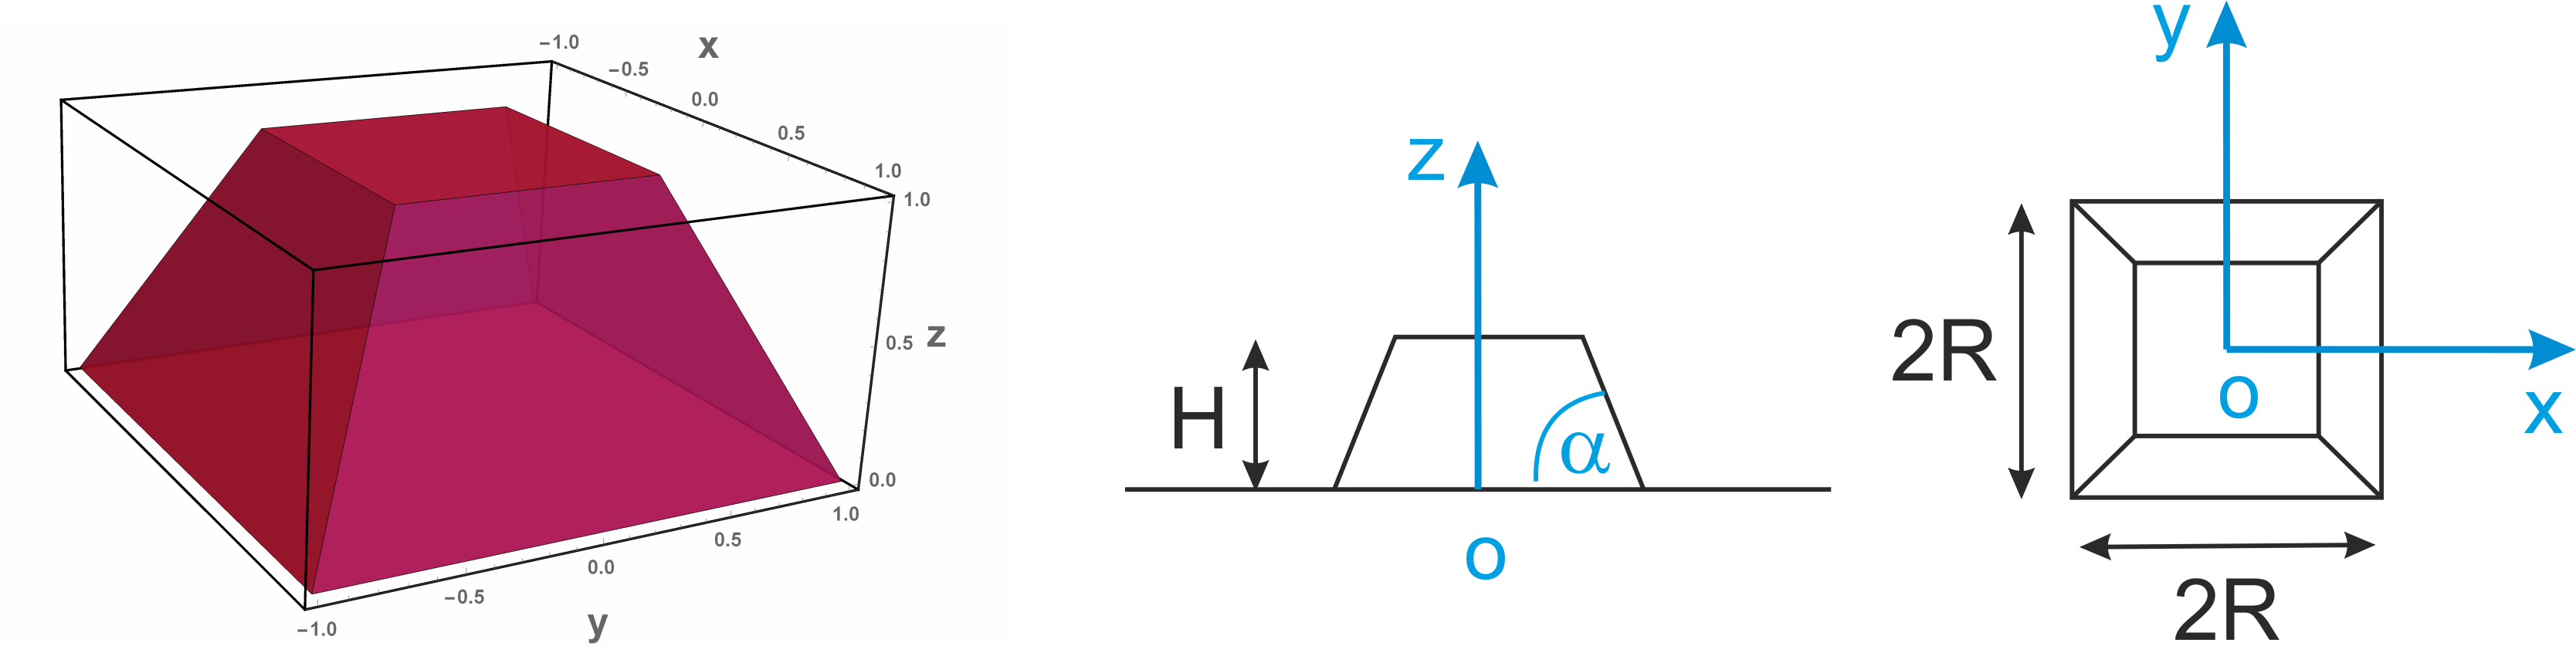
\includegraphics[width=0.9\textwidth]{../images/form_factor/oriented_primitive_opbjects/pyramid4.png}
\end{center}
\caption{unit pyramid with base length of $2R=2$, height $H_R$ and tilting angle $\alpha$.}
\label{fig:opo_pyramid4}
\end{figure}
\begin{align}\label{eq:opo_pyramid4}
\begin{split}
 F_\mathrm{py4}(\mathbf{Q},R,H,\alpha) & = \frac{H}{\tilde{Q}_x\tilde{Q}_y} \bigg\{
        K_1\cos\left(\left(\tilde{Q}_x-\tilde{Q}_y\right)R\right) \\
      & + K_2\sin\left(\left(\tilde{Q}_x-\tilde{Q}_y\right)R\right) \\
      & - K_3\cos\left(\left(\tilde{Q}_x+\tilde{Q}_y\right)R\right) \\
      & - K_4\sin\left(\left(\tilde{Q}_x+\tilde{Q}_y\right)R\right)\bigg\}
\end{split} \\
  q_1 & =\frac12 \left[\frac{\tilde{Q}_x-\tilde{Q}_y}{\tan(\alpha)}+\tilde{Q}_z\right]\\
  q_2 & =\frac12 \left[\frac{\tilde{Q}_x-\tilde{Q}_y}{\tan(\alpha)}-\tilde{Q}_z\right]\\
  q_3 & =\frac12 \left[\frac{\tilde{Q}_x+\tilde{Q}_y}{\tan(\alpha)}+\tilde{Q}_z\right]\\
  q_4 & =\frac12 \left[\frac{\tilde{Q}_x+\tilde{Q}_y}{\tan(\alpha)}-\tilde{Q}_z\right] \\
  K_1 &= \frac{\sin(q_1H)}{q_1H} e^{\imath q_1H}+\frac{\sin(q_2H)}{q_2H} e^{-\imath q_2H}\\
  K_2 &= -\imath \frac{\sin(q_1H)}{q_1H} e^{\imath q_1H}+\imath \frac{\sin(q_2H)}{q_2H} e^{-\imath q_2H}\\
  K_3 &= \frac{\sin(q_3H)}{q_3H} e^{\imath q_3H}+\frac{\sin(q_4H)}{q_4H} e^{-\imath q_4H}\\
  K_4 &= -\imath \frac{\sin(q_3H)}{q_3H} e^{\imath q_3H}+\imath \frac{\sin(q_4H)}{q_4H} e^{-\imath q_4H}\\
  \frac{H}{R} & < \frac{\tan(\alpha)}{\sqrt{3}}
\end{align}

\subsection{oriented superellipsoid} ~\\

\begin{figure}[htb]
\begin{tabular}{ccccc}
  $\epsilon_1=0.1$
    & 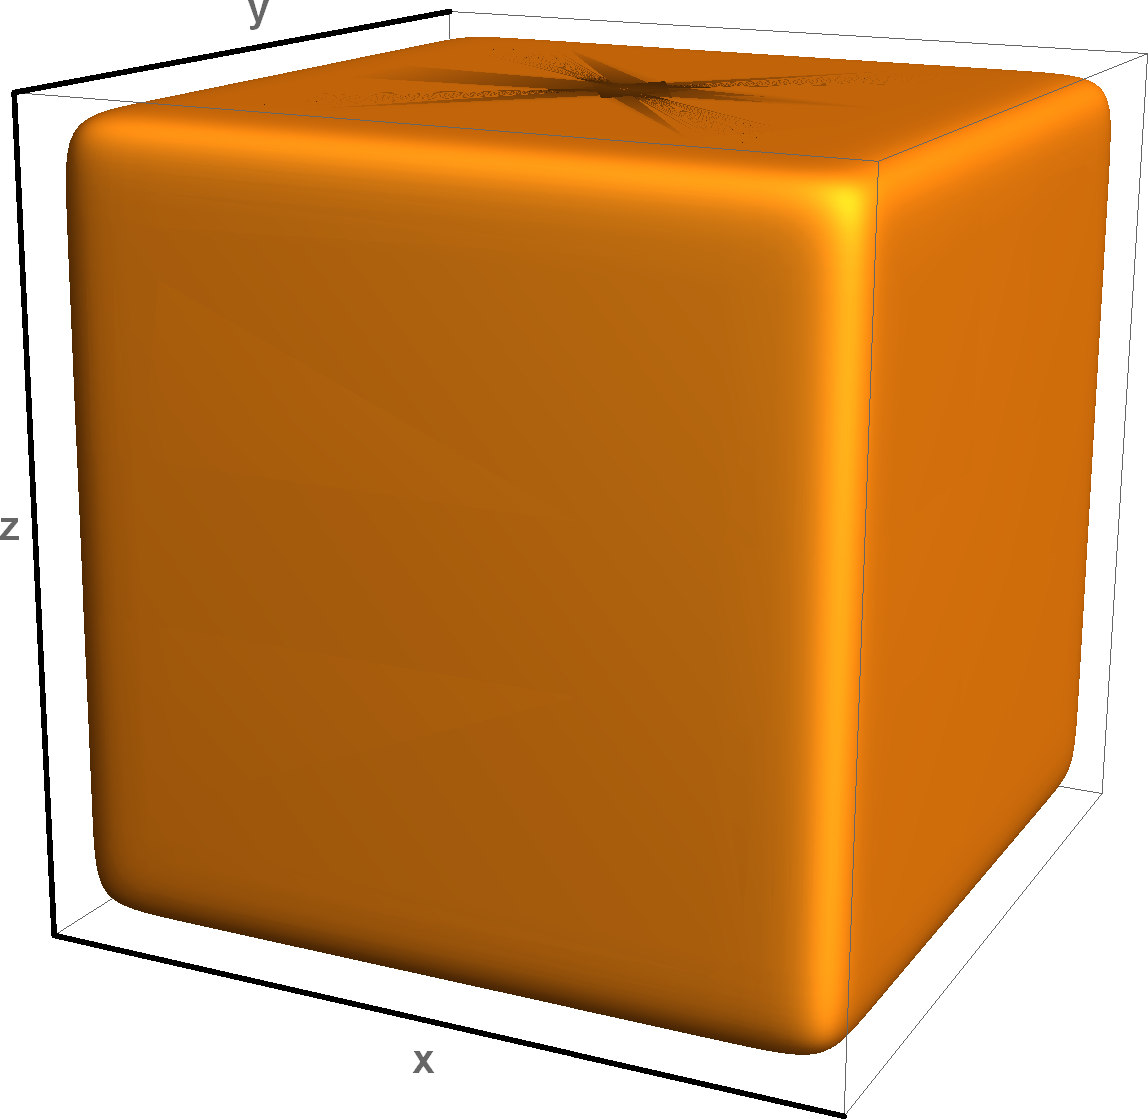
\includegraphics[width=0.2\textwidth]{../images/form_factor/supershapes/superquadric111_01_01.png}
    & 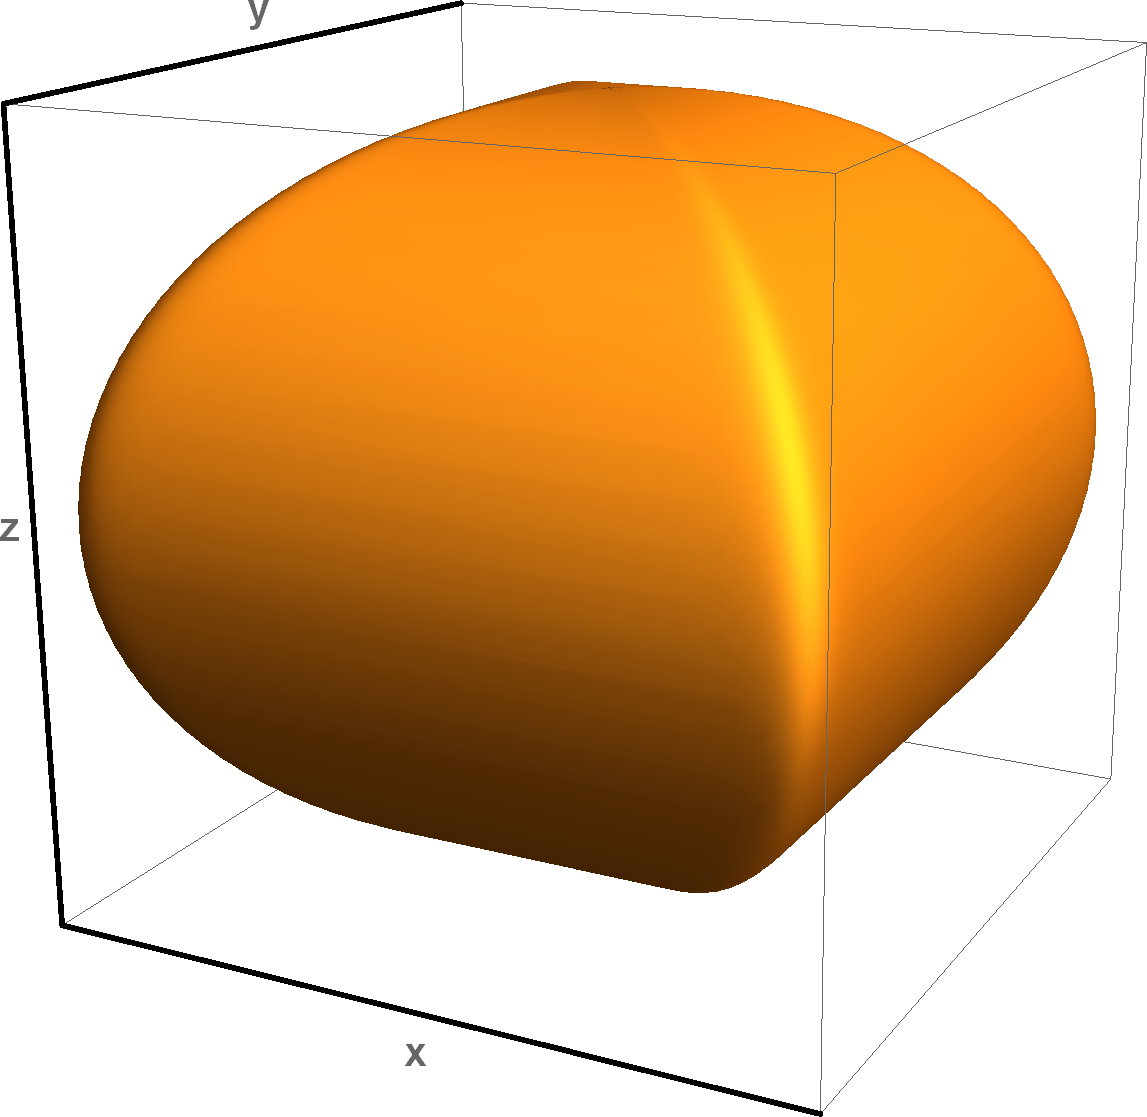
\includegraphics[width=0.2\textwidth]{../images/form_factor/supershapes/superquadric111_01_1.png}
    & 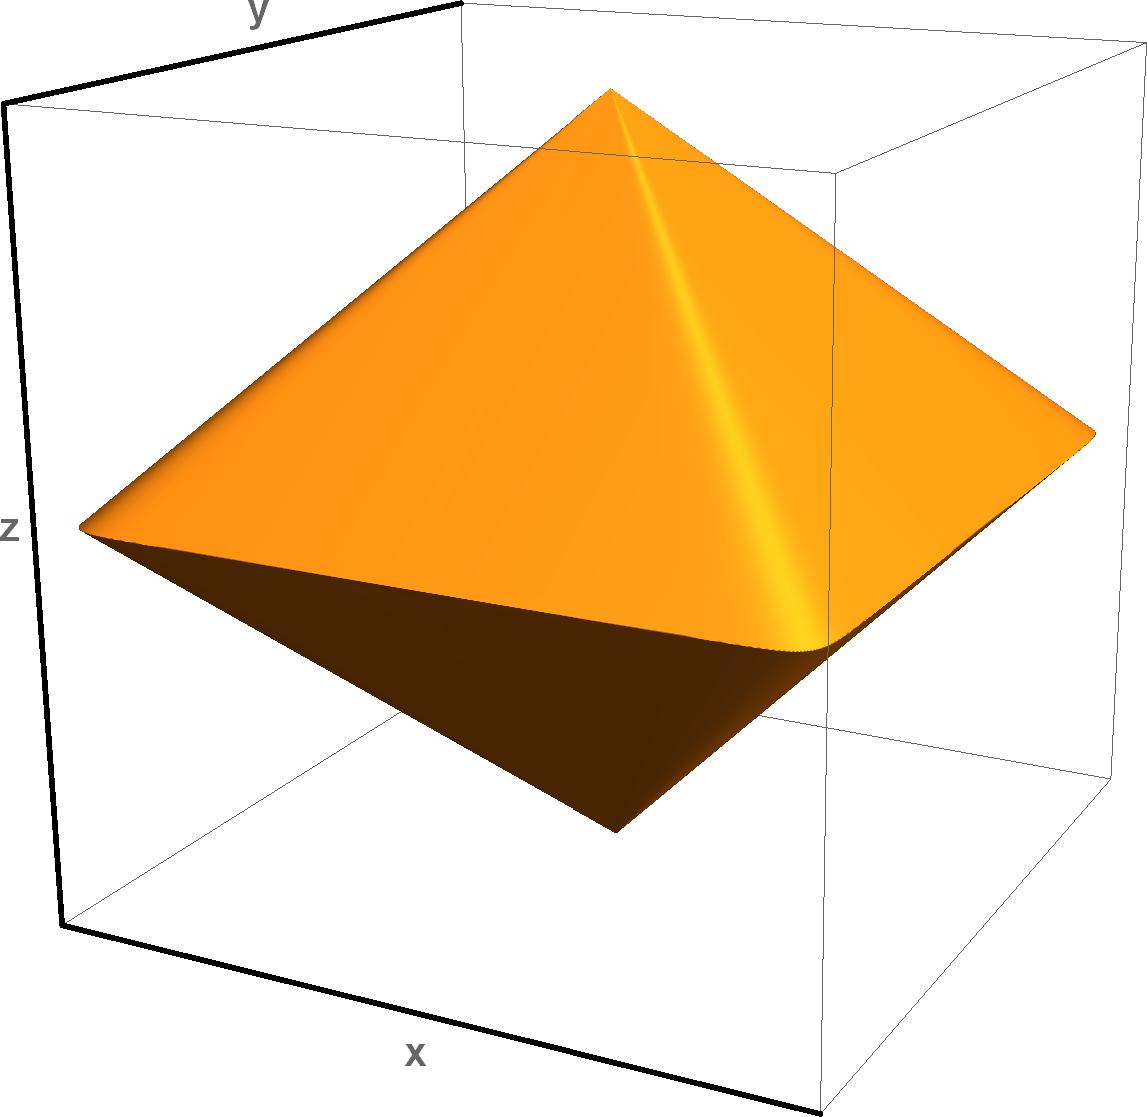
\includegraphics[width=0.2\textwidth]{../images/form_factor/supershapes/superquadric111_01_2.png}
    & 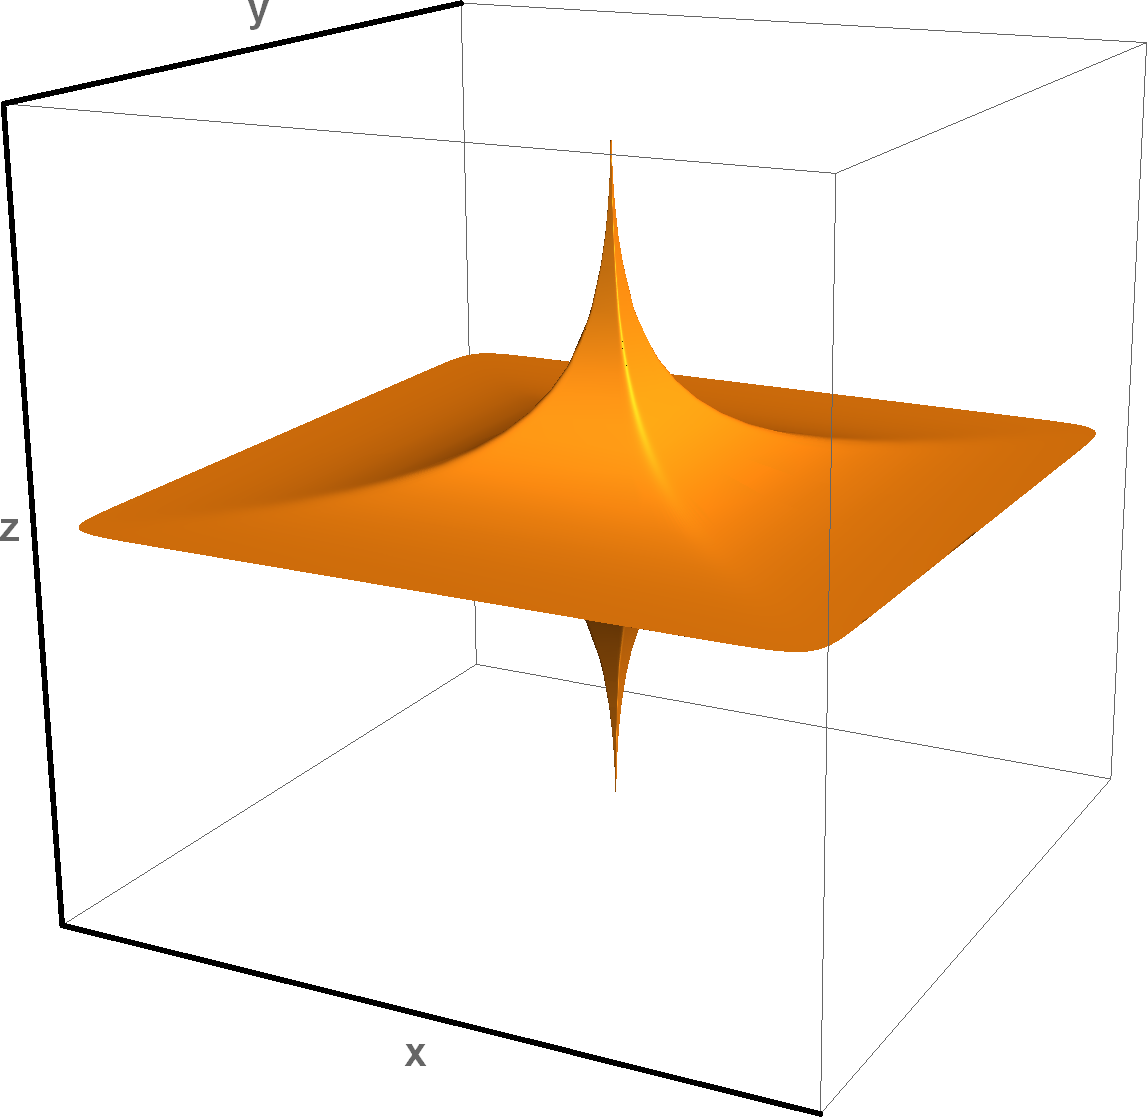
\includegraphics[width=0.2\textwidth]{../images/form_factor/supershapes/superquadric111_01_5.png} \\
  $\epsilon_1=1$
    & 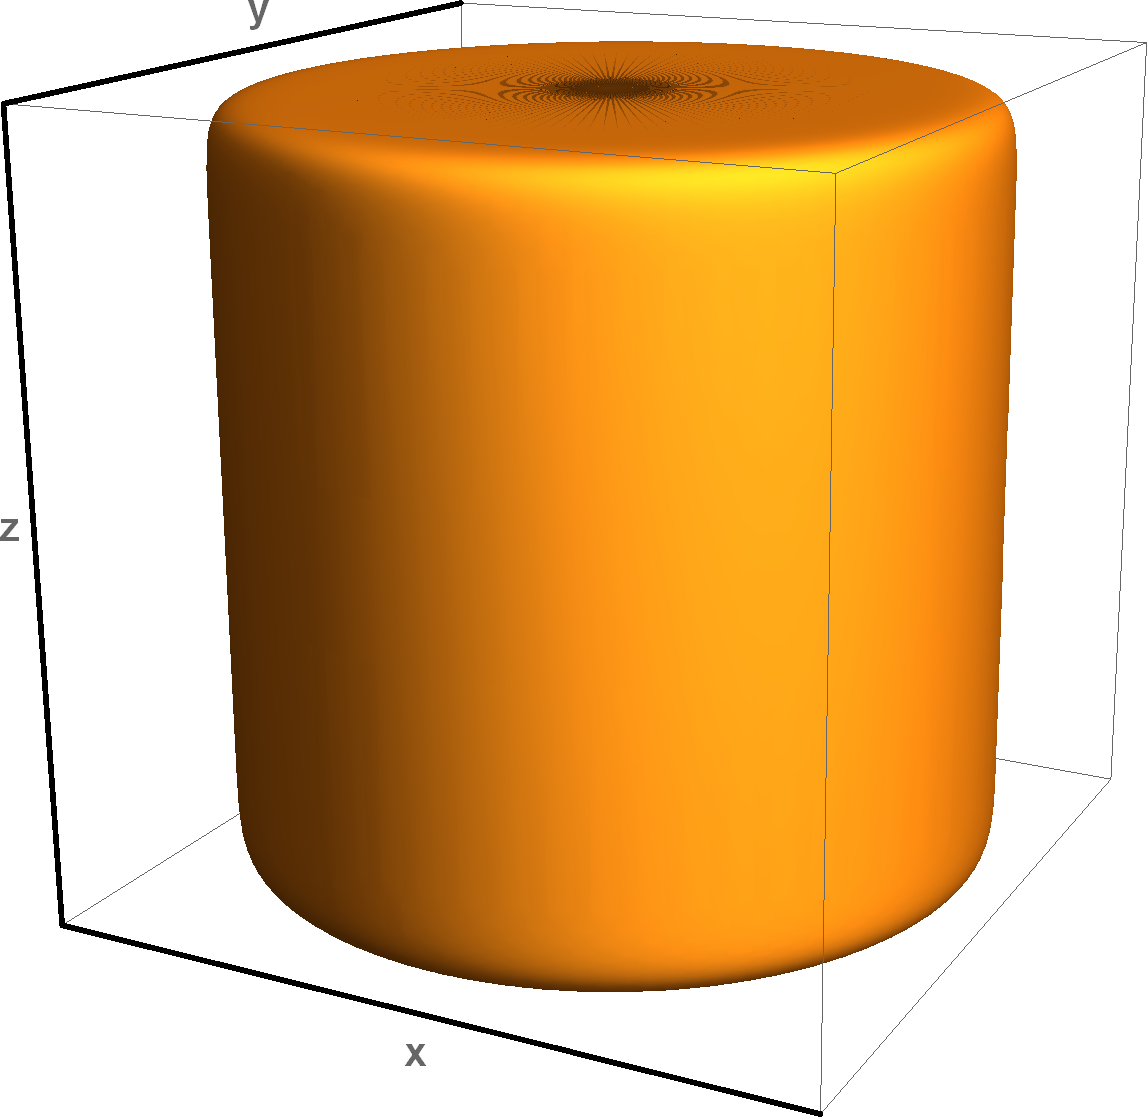
\includegraphics[width=0.2\textwidth]{../images/form_factor/supershapes/superquadric111_1_01.png}
    & 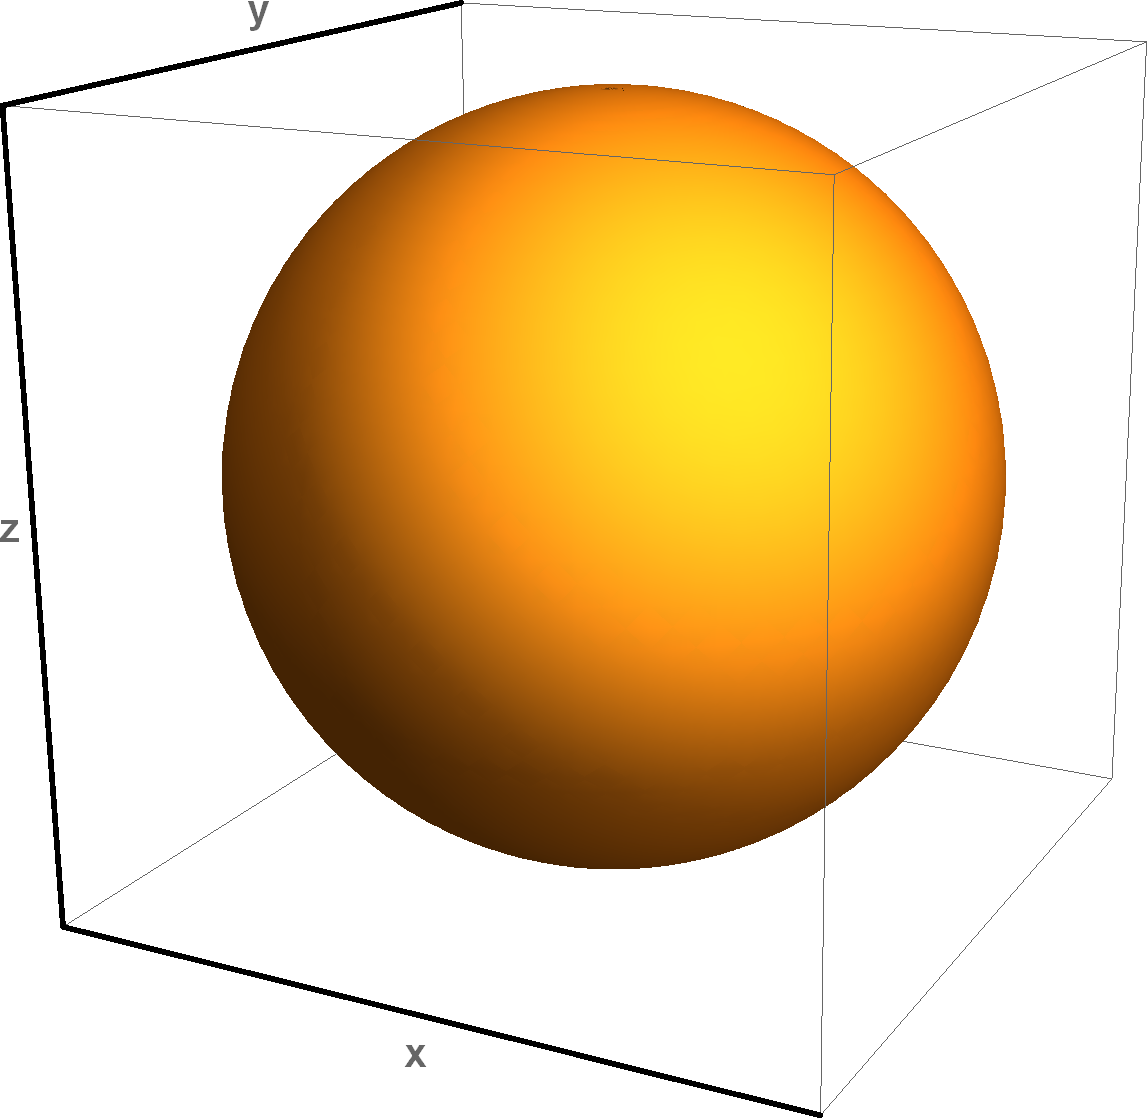
\includegraphics[width=0.2\textwidth]{../images/form_factor/supershapes/superquadric111_1_1.png}
    & 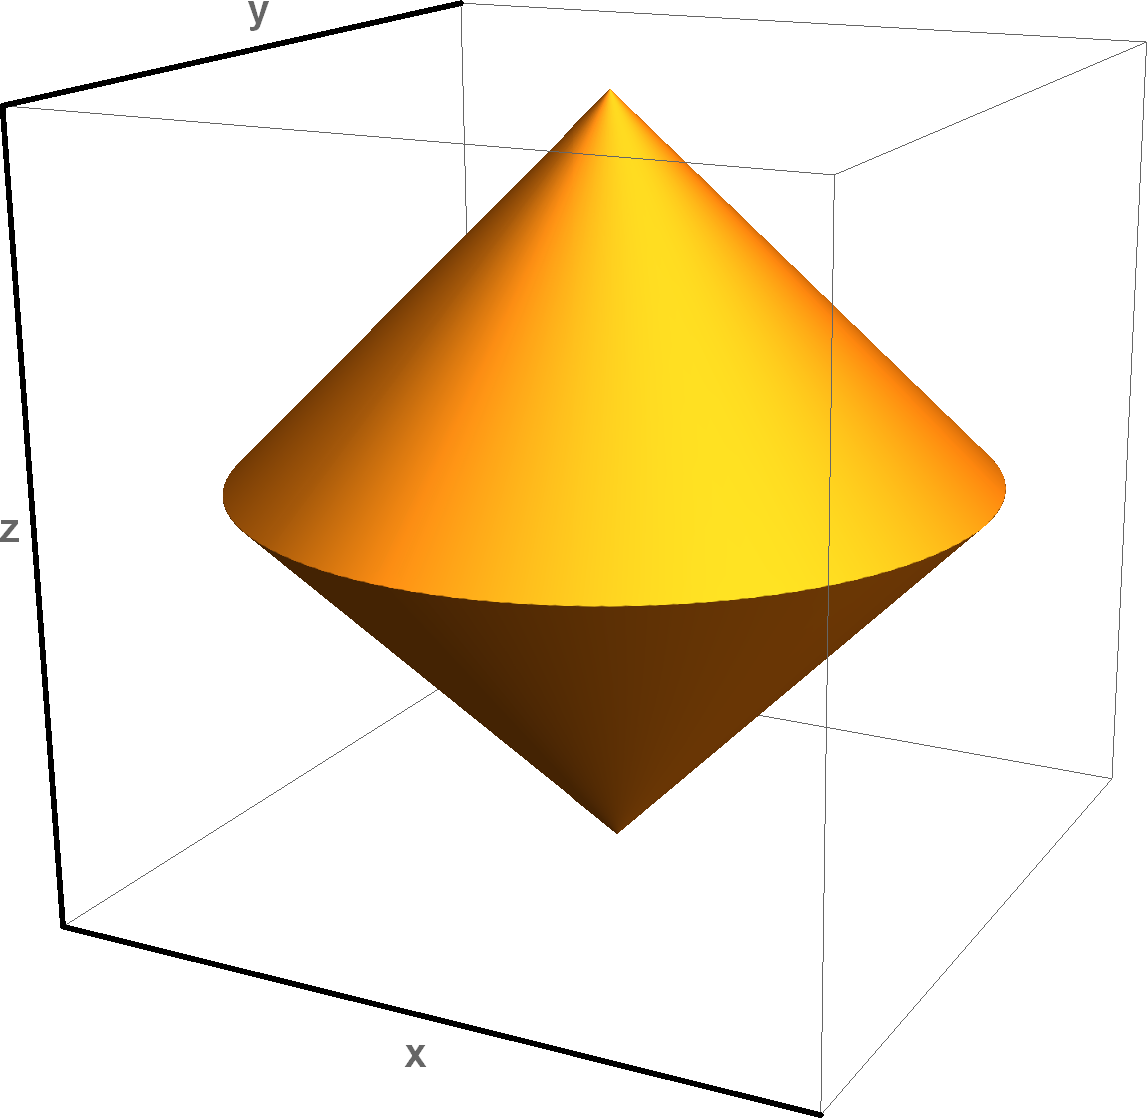
\includegraphics[width=0.2\textwidth]{../images/form_factor/supershapes/superquadric111_1_2.png}
    & 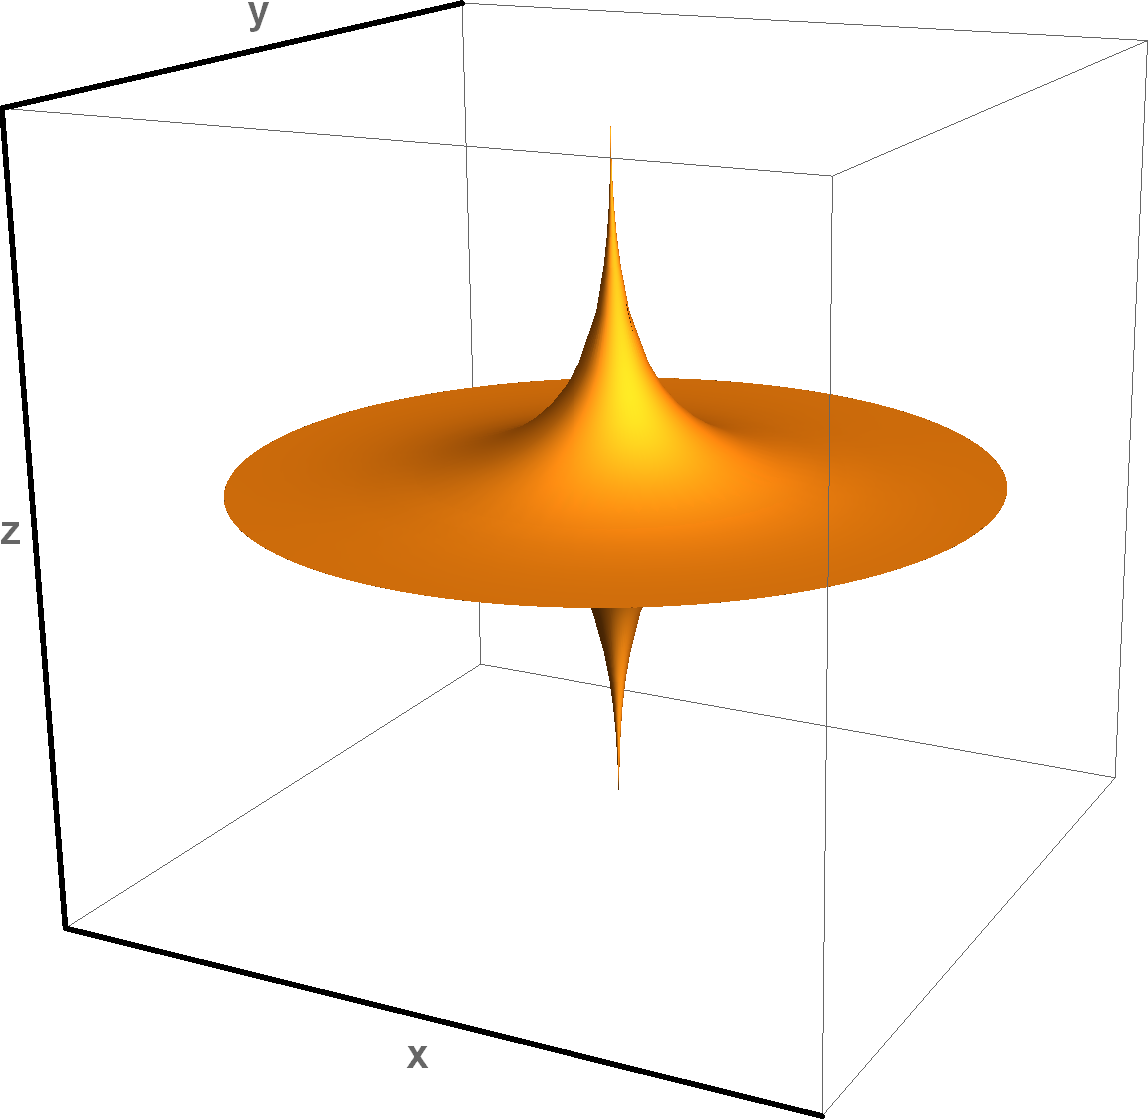
\includegraphics[width=0.2\textwidth]{../images/form_factor/supershapes/superquadric111_1_5.png} \\
  $\epsilon_1=2$
    & 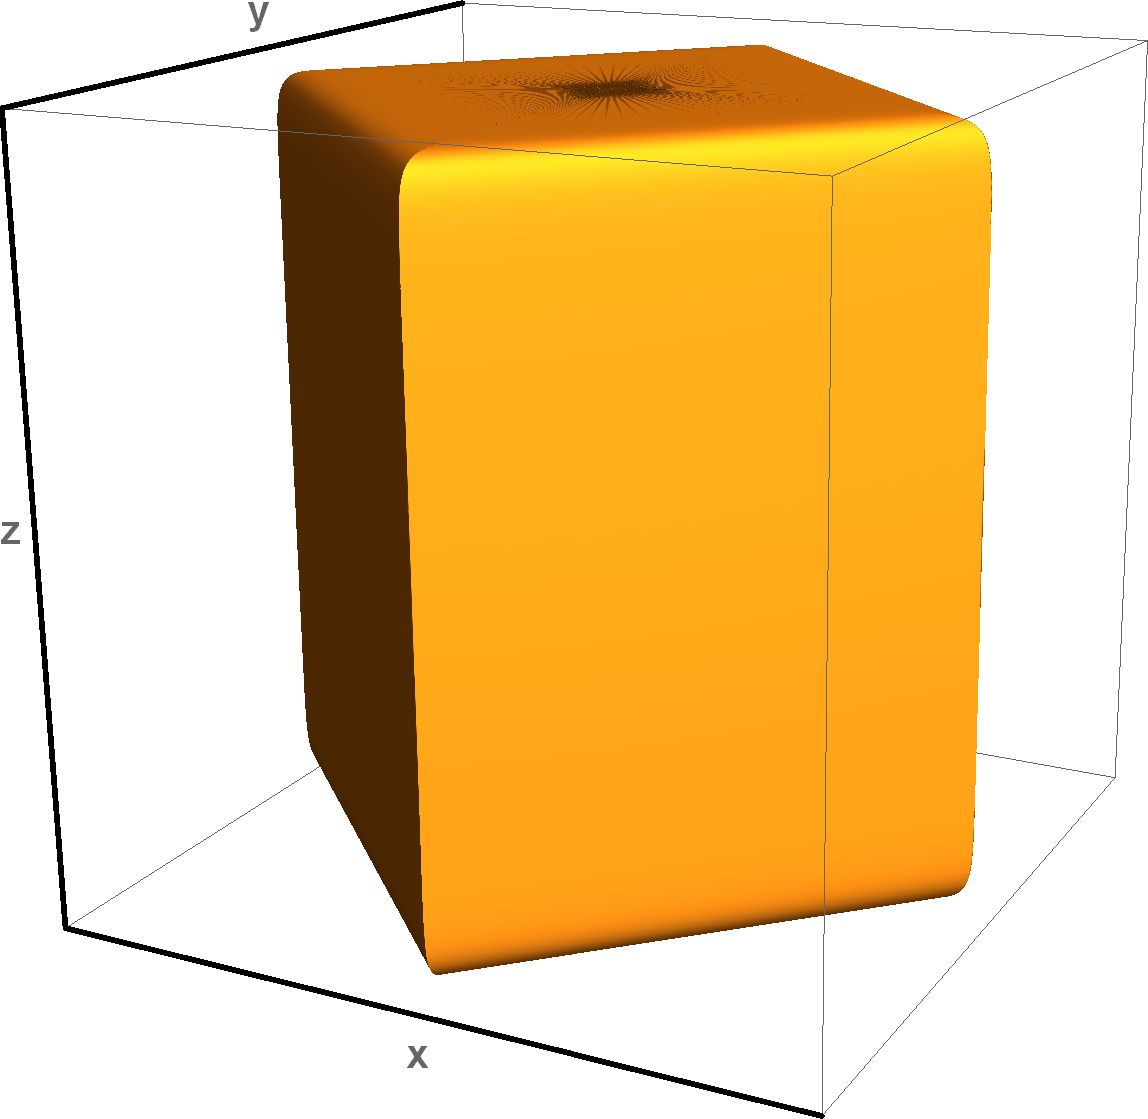
\includegraphics[width=0.2\textwidth]{../images/form_factor/supershapes/superquadric111_2_01.png}
    & 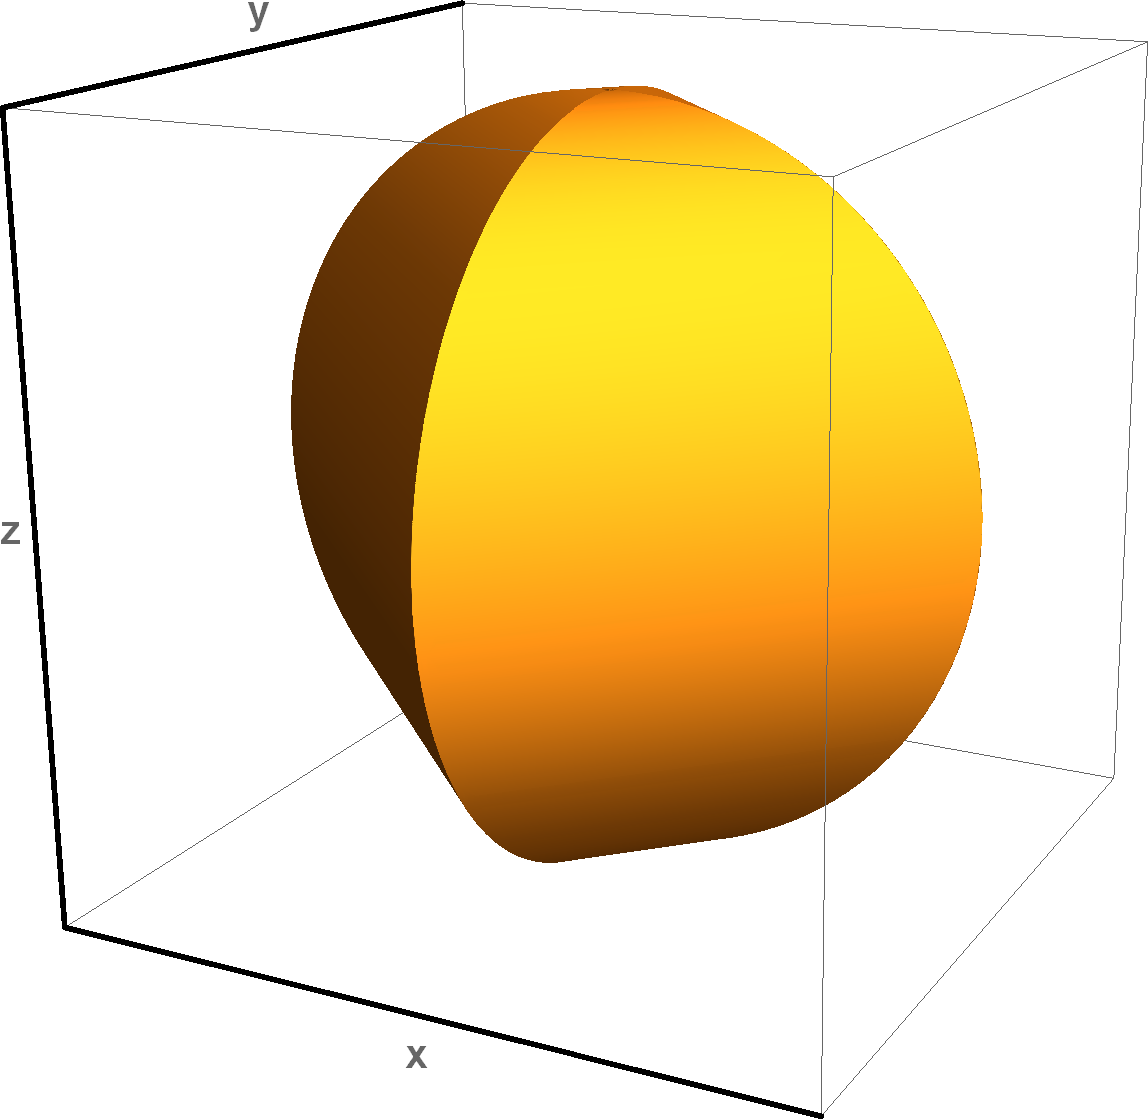
\includegraphics[width=0.2\textwidth]{../images/form_factor/supershapes/superquadric111_2_1.png}
    & 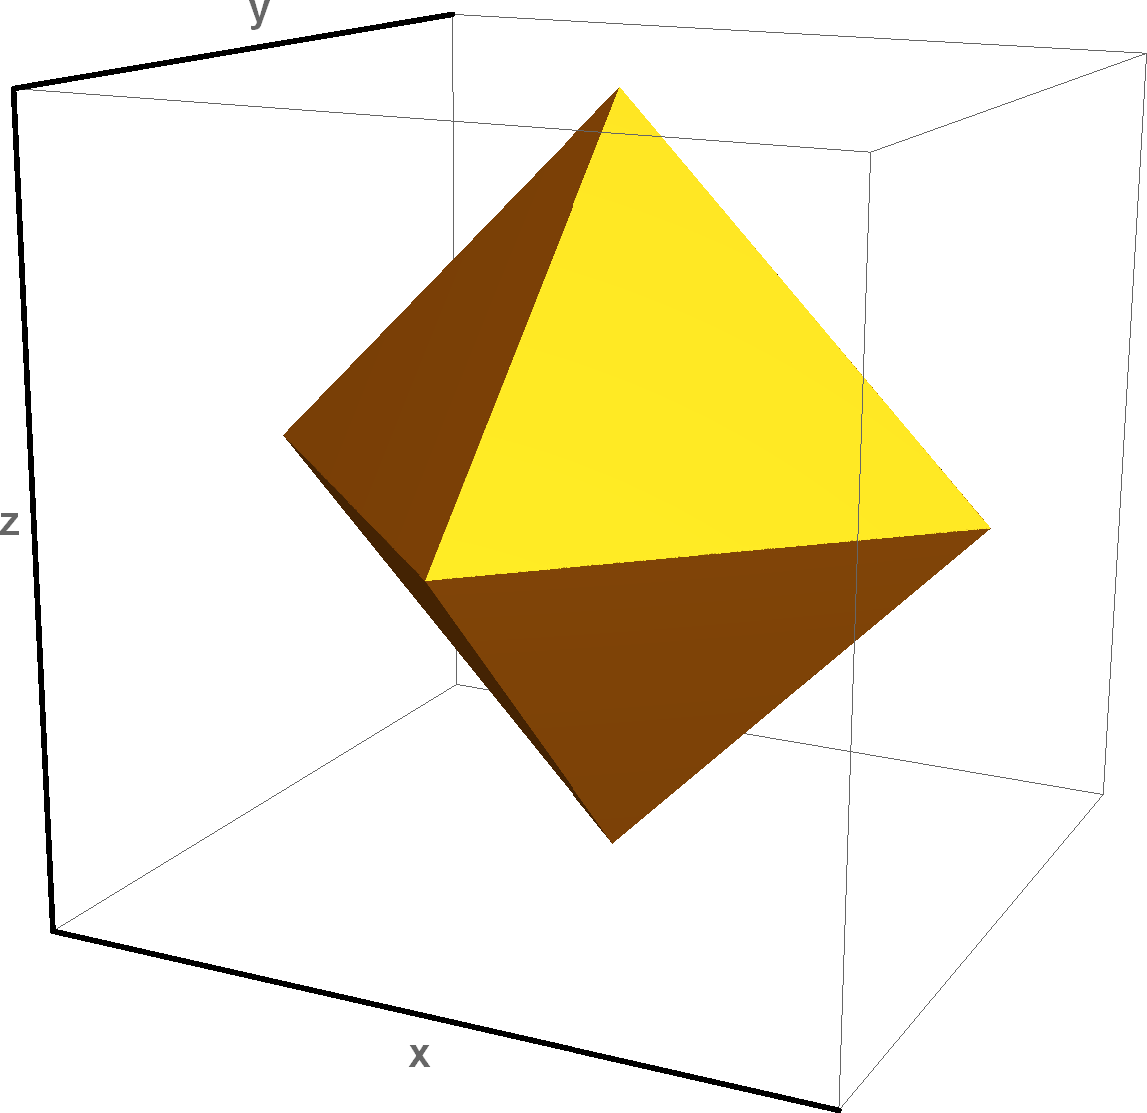
\includegraphics[width=0.2\textwidth]{../images/form_factor/supershapes/superquadric111_2_2.png}
    & 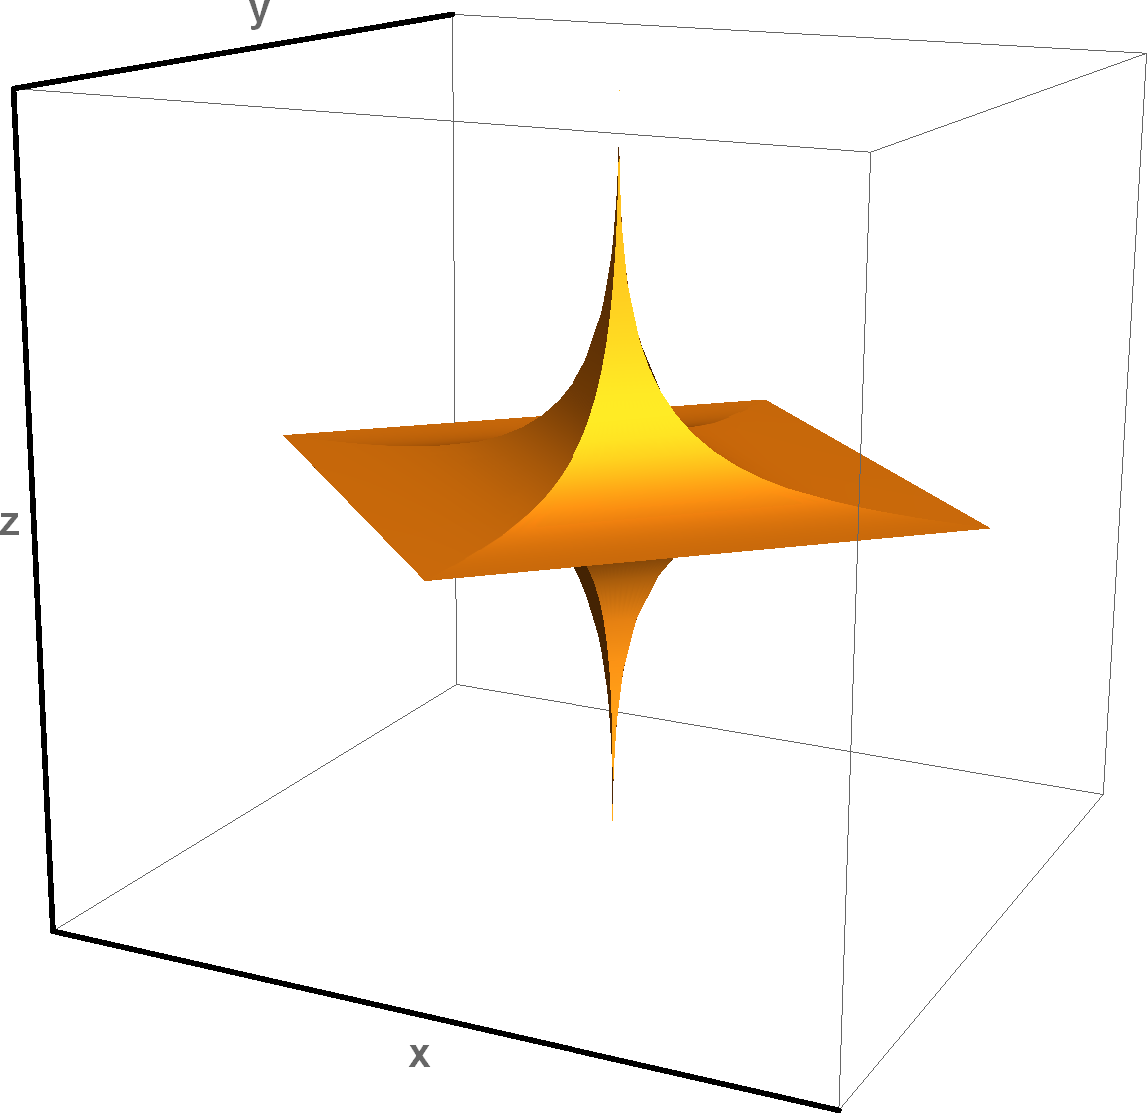
\includegraphics[width=0.2\textwidth]{../images/form_factor/supershapes/superquadric111_2_5.png} \\
  $\epsilon_1=5$
    & 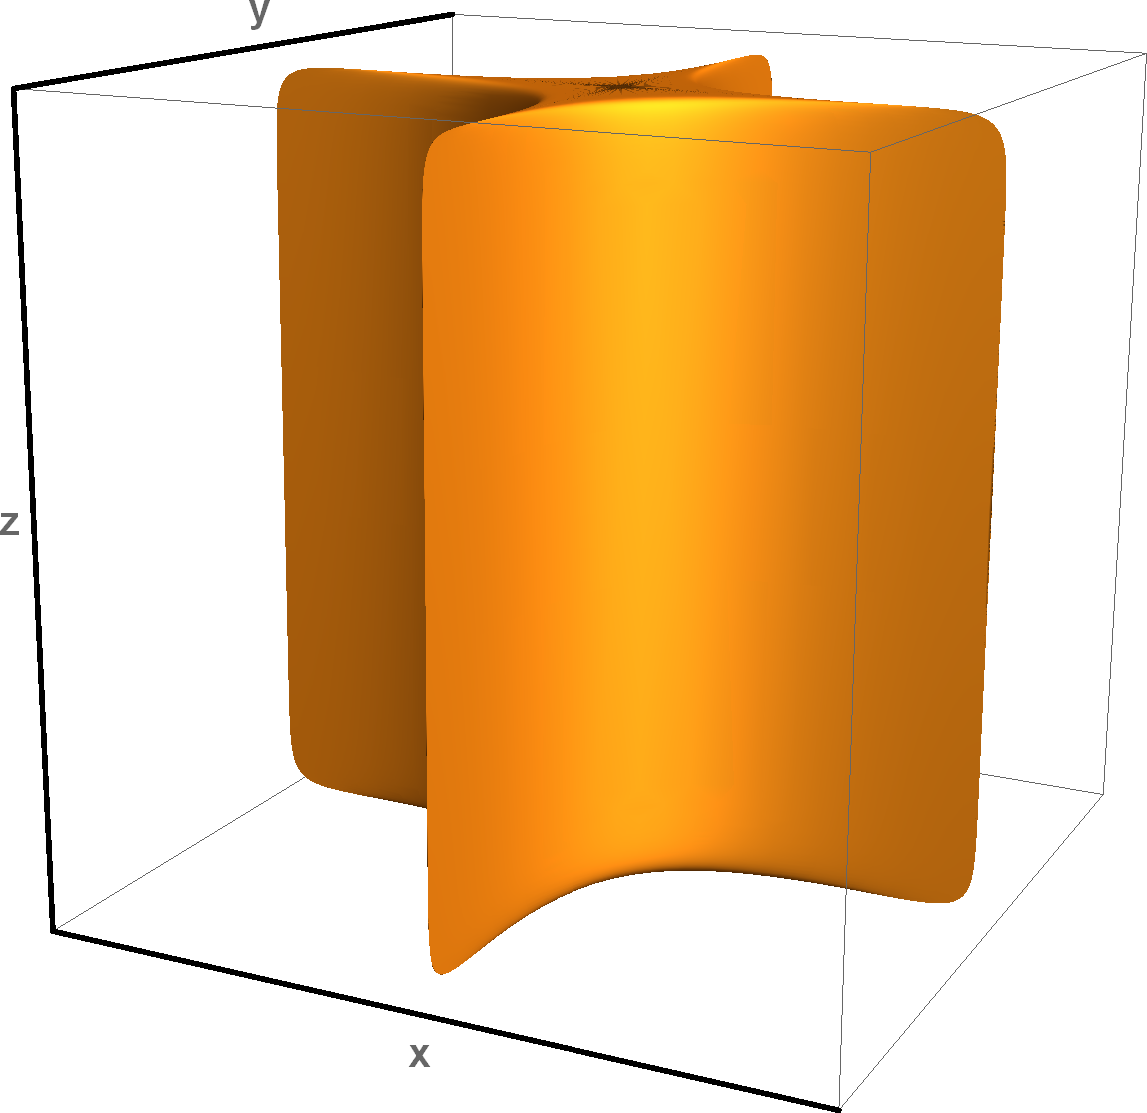
\includegraphics[width=0.2\textwidth]{../images/form_factor/supershapes/superquadric111_5_01.png}
    & 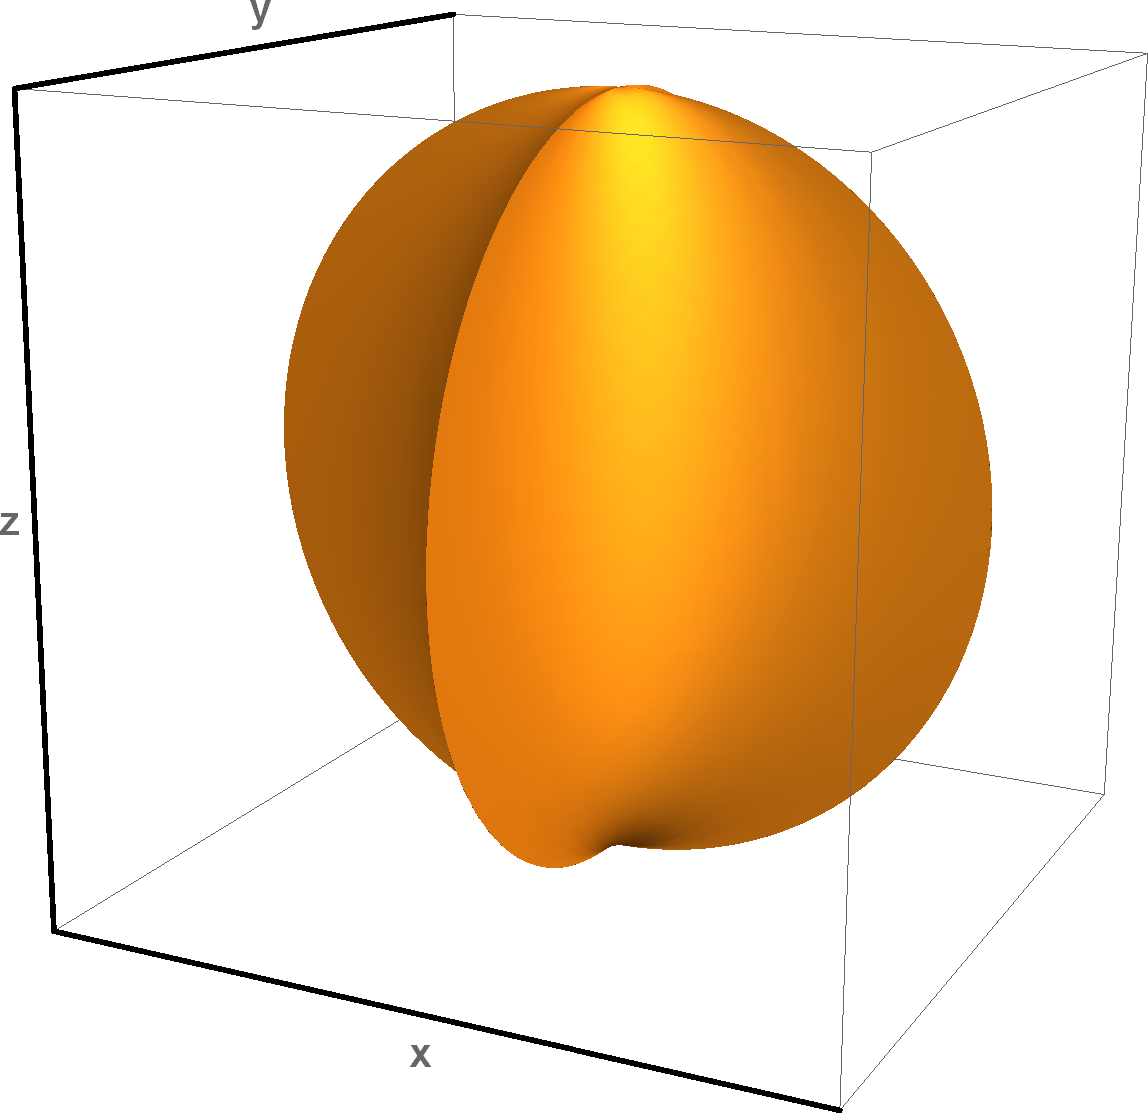
\includegraphics[width=0.2\textwidth]{../images/form_factor/supershapes/superquadric111_5_1.png}
    & 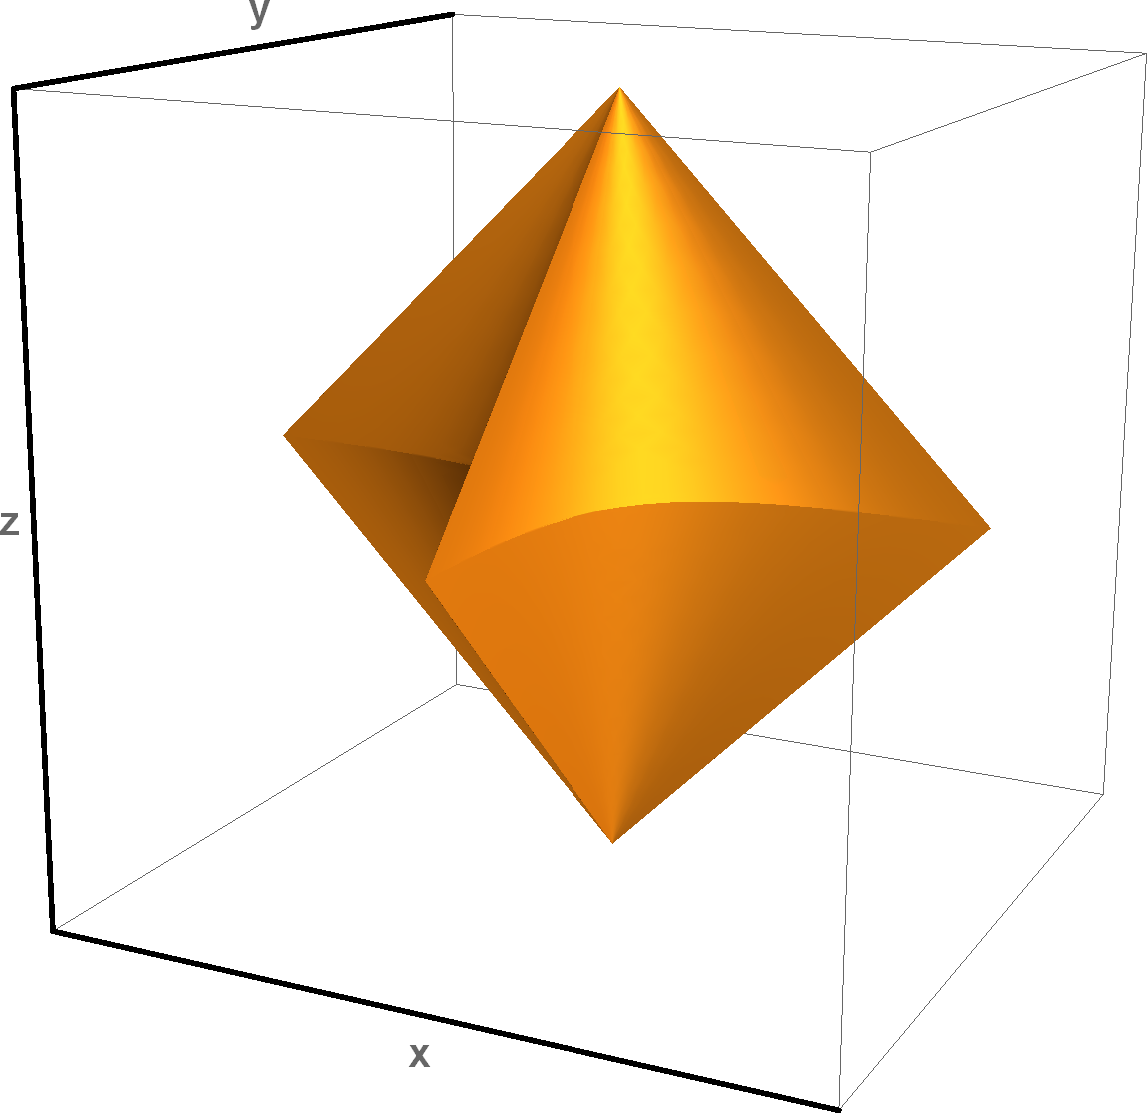
\includegraphics[width=0.2\textwidth]{../images/form_factor/supershapes/superquadric111_5_2.png}
    & \includegraphics[width=0.2\textwidth]{../images/form_factor/supershapes/superquadric111_5_5.png} \\
  & $\epsilon_2=0.1$ & $\epsilon_2=1$ & $\epsilon_2=2$ & $\epsilon_2=5$
\end{tabular}
\caption{Typical superquadrics. The parameters for scale factors are $a_1 = a_2 = a_3 = 1 $. The values for $\epsilon_2$ vary horizontally by $\epsilon_2=0.1, 1,2,5$ and vertically by $\epsilon_1=0.1, 1,2,5$.}
\label{fig:opo_superquadrics}
\end{figure}

Superellipsoids belong to a class of shapes named superquadrics. The class of superquadrics have been widely used in computer graphics and were introduced by \cite{Barr1981}. This class of shapes also include next to superellipsoids so called superhyperboloids and supertoroids. They all have both a
parametric and an implicit representation. The parametric representation of the surface of a superellipsoid is defined by
\begin{align}\label{eq:superellipsoid:parametric}
  \left(
    \begin{array}{c}
      x(a_1\theta,\phi) \\
      y(a_2\theta,\phi) \\
      z(a_3\theta,\phi) \\
    \end{array}
  \right)
 &=
 \left(
    \begin{array}{c}
     a_1 \operatorname{sgnpow}(\cos\theta,\epsilon_2)\operatorname{sgnpow}(\cos\phi,\epsilon_1)  \\
     a_2 \operatorname{sgnpow}(\sin\theta,\epsilon_2)\operatorname{sgnpow}(\cos\phi,\epsilon_1)  \\
     a_3 \operatorname{sgnpow}(\sin\phi,\epsilon_1) \\
    \end{array}
  \right)
\end{align}
whereas the signed power function is defined as
\begin{align}\label{eq:sgnpow}
  \operatorname{sgnpow}(t,\epsilon) &= \operatorname{sgn}(t)\abs{t}^\epsilon \\
  \operatorname{sgn}(t) &=
  \begin{cases}
    -1&{\text{if }}x<0,\\
     0&{\text{if }}x=0,\\
     1&{\text{if }}x>0.
  \end{cases}
\end{align}
The implicit representation is given by
\begin{align}\label{eq:superellipsoid:implicit}
\left(
     \abs{\frac{x}{a_1}}^{\frac{2}{\epsilon_2}}+
     \abs{\frac{y}{a_2}}^{\frac{2}{\epsilon_2}}
\right)^{\frac{\epsilon_2}{\epsilon_1}} +
\abs{\frac{z}{a_3}}^{\frac{2}{\epsilon_1}} &\leq 1
\end{align}
A supersphere is a special case of superellipsoid for which the two exponents are equal $\epsilon_1=\epsilon_2$. The implicit representation then reads as
$\abs{\frac{x}{a_1}}^n+\abs{\frac{y}{a_2}}^n+\abs{\frac{y}{a_3}}^n\leq 1$ with $n=1/\epsilon_1=1/\epsilon_2$.
Another special case is the superegg for which one exponent is equal $\epsilon_1=1$ and the implicit representation then reads as
$\left(\abs{\frac{x}{a_1}}^2+\abs{\frac{y}{a_2}}^2\right)^{1/\epsilon_2}+\abs{\frac{y}{a_3}}^{2/\epsilon_2}\leq 1$.
As the asymmetric superellipsoid is obtained by a scale transform, which is a special case of an affine transform only the Fourier transform of a unit superellipsoid has to be solved. All its affine transform than can be easily calculated by linear algebra.


\begin{figure}[thb]
\begingroup
\setlength{\tabcolsep}{1pt}
\def\arraystretch{0.4}%
 \captionsetup[subfigure]{position=b}
\centering
\subcaptionbox{$(\epsilon_1,\epsilon_2)=(1,2)$ \label{fig:superquadricsIQ2D_1}}{
\begin{tabular}{llll}
%\toprule  \\ %\midrule
2m   & \includegraphics[width=0.13\textwidth]{../images/form_factor/supershapes/superquadrics_1_2_0_0_0_2m.png}
     & \includegraphics[width=0.13\textwidth]{../images/form_factor/supershapes/superquadrics_1_2_0_90_0_2m.png}
     & \includegraphics[width=0.13\textwidth]{../images/form_factor/supershapes/superquadrics_1_2_0_45_45_2m.png}  \\
6m   & \includegraphics[width=0.13\textwidth]{../images/form_factor/supershapes/superquadrics_1_2_0_0_0_6m.png}
     & \includegraphics[width=0.13\textwidth]{../images/form_factor/supershapes/superquadrics_1_2_0_90_0_6m.png}
     & \includegraphics[width=0.13\textwidth]{../images/form_factor/supershapes/superquadrics_1_2_0_45_45_6m.png}  \\
18m  & \includegraphics[width=0.13\textwidth]{../images/form_factor/supershapes/superquadrics_1_2_0_0_0_18m.png}
     & \includegraphics[width=0.13\textwidth]{../images/form_factor/supershapes/superquadrics_1_2_0_90_0_18m.png}
     & \includegraphics[width=0.13\textwidth]{../images/form_factor/supershapes/superquadrics_1_2_0_45_45_18m.png}  \\
%\diagbox{sampl.-det.}{$(\alpha,\beta,\gamma)$}
     & {\small $(0^\circ,0^\circ,0^\circ)$}
     & {\small $(0^\circ,90^\circ,0^\circ)$}
     & {\small $(0^\circ,45^\circ,45^\circ)$}  %\bottomrule
\end{tabular}
}
\hfill
\subcaptionbox{$(\epsilon_1,\epsilon_2)=(2,0.1)$ \label{fig:superquadricsIQ2D_2}}{
\begin{tabular}{llll}
%\toprule
2m   & \includegraphics[width=0.13\textwidth]{../images/form_factor/supershapes/superquadrics_2_01_0_0_0_2m.png}
     & \includegraphics[width=0.13\textwidth]{../images/form_factor/supershapes/superquadrics_2_01_0_90_0_2m.png}
     & \includegraphics[width=0.13\textwidth]{../images/form_factor/supershapes/superquadrics_2_01_0_45_45_2m.png}  \\
6m   & \includegraphics[width=0.13\textwidth]{../images/form_factor/supershapes/superquadrics_2_01_0_0_0_6m.png}
     & \includegraphics[width=0.13\textwidth]{../images/form_factor/supershapes/superquadrics_2_01_0_90_0_6m.png}
     & \includegraphics[width=0.13\textwidth]{../images/form_factor/supershapes/superquadrics_2_01_0_45_45_6m.png}  \\
18m  & \includegraphics[width=0.13\textwidth]{../images/form_factor/supershapes/superquadrics_2_01_0_0_0_18m.png}
     & \includegraphics[width=0.13\textwidth]{../images/form_factor/supershapes/superquadrics_2_01_0_90_0_18m.png}
     & \includegraphics[width=0.13\textwidth]{../images/form_factor/supershapes/superquadrics_2_01_0_45_45_18m.png}  \\
%\diagbox{sampl.-det.}{$(\alpha,\beta,\gamma)$}
     & {\small $(0^\circ,0^\circ,0^\circ)$}
     & {\small $(0^\circ,90^\circ,0^\circ)$}
     & {\small $(0^\circ,45^\circ,45^\circ)$}  %\bottomrule
\end{tabular}
}

\vspace{5mm}

\subcaptionbox{$(\epsilon_1,\epsilon_2)=(1,2)$ \label{fig:superquadricsIQ2D_3}}{
\begin{tabular}{llll}
%\toprule
2m   & \includegraphics[width=0.13\textwidth]{../images/form_factor/supershapes/superquadrics_2_2_0_0_0_2m.png}
     & \includegraphics[width=0.13\textwidth]{../images/form_factor/supershapes/superquadrics_2_2_0_90_0_2m.png}
     & \includegraphics[width=0.13\textwidth]{../images/form_factor/supershapes/superquadrics_2_2_0_45_45_2m.png}  \\
6m   & \includegraphics[width=0.13\textwidth]{../images/form_factor/supershapes/superquadrics_2_2_0_0_0_6m.png}
     & \includegraphics[width=0.13\textwidth]{../images/form_factor/supershapes/superquadrics_2_2_0_90_0_6m.png}
     & \includegraphics[width=0.13\textwidth]{../images/form_factor/supershapes/superquadrics_2_2_0_45_45_6m.png}  \\
18m  & \includegraphics[width=0.13\textwidth]{../images/form_factor/supershapes/superquadrics_2_2_0_0_0_18m.png}
     & \includegraphics[width=0.13\textwidth]{../images/form_factor/supershapes/superquadrics_2_2_0_90_0_18m.png}
     & \includegraphics[width=0.13\textwidth]{../images/form_factor/supershapes/superquadrics_2_2_0_45_45_18m.png}  \\
%\diagbox{sampl.-det.}{$(\alpha,\beta,\gamma)$}
     & {\small $(0^\circ,0^\circ,0^\circ)$}
     & {\small $(0^\circ,90^\circ,0^\circ)$}
     & {\small $(0^\circ,45^\circ,45^\circ)$}  %\bottomrule
\end{tabular}
}
\hfill
\subcaptionbox{$(\epsilon_1,\epsilon_2)=(2,0.1)$ \label{fig:superquadricsIQ2D_4}}{
\begin{tabular}{llll}
%\toprule
2m   & \includegraphics[width=0.13\textwidth]{../images/form_factor/supershapes/superquadrics_2_5_0_0_0_2m.png}
     & \includegraphics[width=0.13\textwidth]{../images/form_factor/supershapes/superquadrics_2_5_0_90_0_2m.png}
     & \includegraphics[width=0.13\textwidth]{../images/form_factor/supershapes/superquadrics_2_5_0_45_45_2m.png}  \\
6m   & \includegraphics[width=0.13\textwidth]{../images/form_factor/supershapes/superquadrics_2_5_0_0_0_6m.png}
     & \includegraphics[width=0.13\textwidth]{../images/form_factor/supershapes/superquadrics_2_5_0_90_0_6m.png}
     & \includegraphics[width=0.13\textwidth]{../images/form_factor/supershapes/superquadrics_2_5_0_45_45_6m.png}  \\
18m  & \includegraphics[width=0.13\textwidth]{../images/form_factor/supershapes/superquadrics_2_5_0_0_0_18m.png}
     & \includegraphics[width=0.13\textwidth]{../images/form_factor/supershapes/superquadrics_2_5_0_90_0_18m.png}
     & \includegraphics[width=0.13\textwidth]{../images/form_factor/supershapes/superquadrics_2_5_0_45_45_18m.png}  \\
%\diagbox{sampl.-det.}{$(\alpha,\beta,\gamma)$}
     & {\small $(0^\circ,0^\circ,0^\circ)$}
     & {\small $(0^\circ,90^\circ,0^\circ)$}
     & {\small $(0^\circ,45^\circ,45^\circ)$}  %\bottomrule
\end{tabular}
}
\endgroup
  \caption{Scattering patterns for super-quadrics with scale factors are $a_1=30$nm, $a_2=20$nm, $a_3=10$nm calculated for detector distances (2m, 6m, 18m) and a wavelength of 0.6nm are shown. Three orientation using Tait–Bryan angles (yaw-
pitch-roll) are shown.} \label{fig:superquadricsIQ2D}
\end{figure}

The Fourier transform of a unit super-quadrics ($a_1=a_2=a_3=1$) is
\begin{align}\label{eq:FTsuperellipsoid}
  F_\mathrm{SEll}(\B{Q}) &=
\det(\M{D}^{-1})\, e^{-\imath\B{QR}}\, \Delta\eta\, \int\limits_{-1}^1
\mathrm{d}x\, \int\limits_{-Y(x)}^{Y(x)} \mathrm{d}y\,  \int\limits_{-Z(x,y)}^{Z(x,y)} \mathrm{d}z \,
e^{\imath\B{\hat{Q}r}} \nonumber \\
 &=
\det(\M{D}^{-1})\, e^{-\imath\B{QR}}\, \Delta\eta\,   \\
& \times \int\limits_{-1}^1
\mathrm{d}x\, \int\limits_{-Y(x)}^{Y(x)} \mathrm{d}y\,
e^{\imath\left(\hat{Q}_xx+\hat{Q}_yy\right)} 2Z(x,y)\operatorname{sinc}(\hat{Q}_z Z(x,y))\nonumber \\
&= \det(\M{D}^{-1})\, e^{-\imath\B{QR}}\, \Delta\eta\, \\
& \times \int\limits_{-1}^1
\mathrm{d}x\, \int\limits_{-1}^{1} \mathrm{d}s\,
e^{\imath\left(\hat{Q}_xx+\hat{Q}_yY(x)s\right)} 2Z(x,Y(x)s)\operatorname{sinc}(\hat{Q}_z Z(x,Y(x)s))Y(x)\nonumber \\
Y(x) &= \left(1-x^{\frac{2}{\epsilon_2}}\right)^{\frac{\epsilon_2}{2}}\\
Z(x,y) &= \left(1-\left(x^{\frac{2}{\epsilon_2}}+y^{\frac{2}{\epsilon_2}}\right)^{\frac{\epsilon_2}{\epsilon_1}}\right)^{\frac{\epsilon_1}{2}}
\end{align}



\clearpage
\subsection{oriented super-egg} ~\\

\begin{figure}[htb]
\begin{tabular}{ccccc}
     \includegraphics[width=0.18\textwidth]{../images/form_factor/supershapes/SuperEggPietHein.png}
    & \includegraphics[width=0.18\textwidth]{../images/form_factor/supershapes/SuperEgg08.png}
    & \includegraphics[width=0.18\textwidth]{../images/form_factor/supershapes/SuperEgg1.png}
    & \includegraphics[width=0.18\textwidth]{../images/form_factor/supershapes/SuperEgg2.png}
    & \includegraphics[width=0.18\textwidth]{../images/form_factor/supershapes/SuperEgg5.png} \\
     $\epsilon_1=0.4$ & $\epsilon_1=0.8$ & $\epsilon_1=1$ & $\epsilon_1=2$ & $\epsilon_1=5$
\end{tabular}
\caption{Supereggs. The parameters for the scale factors of the shown supereggs are $a = b = \frac34 c $. The values for $\epsilon_2=2$ and $\epsilon_1=0.4, 0.8, 1,2,5$.}
\label{fig:opo_superegg}
\end{figure}

The superegg is a superellipsoid whose horizontal cross-sections are ellipses, i.e. $\epsilon_2=1$. It is defined by the inequality \cite{WeisssteinSuperEgg}
\begin{align}
\label{eq:superegg_implicit}
   \left(\sqrt{\left(\frac{x}{a_1}\right)^2+\left(\frac{y}{a_2}\right)^2}\right)^{\frac{2}{\epsilon1}} + \left(\frac{z}{a_3}\right)^{\frac{2}{\epsilon1}} & \leq 1
\end{align}
For circular cross-sections the Fourier transform \cite{Maric2017} can be written as a single integral. For the more general case of an elliptical cross-section the Fourier transform still can be written as a single integral, however, the orientation average becomes a double integral as the cylinder symmetry get lost.
\begin{align}
F_\mathrm{SEgg}(\B{Q}) &=
\det(\M{D}^{-1})\, e^{-\imath\B{QR}}\, \Delta\eta\,  \nonumber \\
 &\times \int_0^1 \frac{4 \pi  r \sin \left(\hat{Q}_z \left(1-r^{2/\epsilon_1}\right)^{\epsilon_1/2}\right) \operatorname{J}_0\left(\sqrt{\hat{Q}_x^2+\hat{Q}_y^2}
   r\right)}{\hat{Q}_z} \mathrm{d}r
\end{align}
Alternatively by using a different variable transformation the form factor can also be written as \cite{Maric2017}
\begin{align}
F_\mathrm{SEgg}(\B{Q}) &=
\det(\M{D}^{-1})\, e^{-\imath\B{QR}}\, \Delta\eta\,  \nonumber \\
 &\times \int_0^1 4 \pi  r^2(z) \frac{\operatorname{J}_1\left(r(z)\sqrt{\hat{Q}_x^2+\hat{Q}_y^2}\right) }{r(z)\sqrt{\hat{Q}_x^2+\hat{Q}_y^2}} \cos\left(z\hat{Q}_z\right)  \mathrm{d}z \\
 r(z) &=\left(1-z^{2/\epsilon_1}\right)^{\epsilon_1/2}
\end{align}

\begin{figure}[htb]
\begin{center}
\begin{tabular}{llllll}
%\toprule
{\small $(0^\circ,0^\circ,0^\circ)$}
     & \includegraphics[width=0.15\textwidth]{../images/form_factor/supershapes/superegg_0_0_0_18m_0p1.png}
     & \includegraphics[width=0.15\textwidth]{../images/form_factor/supershapes/superegg_0_0_0_18m_0p4.png}
     & \includegraphics[width=0.15\textwidth]{../images/form_factor/supershapes/superegg_0_0_0_18m_1p0.png}
     & \includegraphics[width=0.15\textwidth]{../images/form_factor/supershapes/superegg_0_0_0_18m_2p0.png}
     & \includegraphics[width=0.15\textwidth]{../images/form_factor/supershapes/superegg_0_0_0_18m_5p0.png}  \\
{\small $(0^\circ,90^\circ,0^\circ)$}
     & \includegraphics[width=0.15\textwidth]{../images/form_factor/supershapes/superegg_0_90_0_18m_0p1.png}
     & \includegraphics[width=0.15\textwidth]{../images/form_factor/supershapes/superegg_0_90_0_18m_0p4.png}
     & \includegraphics[width=0.15\textwidth]{../images/form_factor/supershapes/superegg_0_90_0_18m_1p0.png}
     & \includegraphics[width=0.15\textwidth]{../images/form_factor/supershapes/superegg_0_90_0_18m_2p0.png}
     & \includegraphics[width=0.15\textwidth]{../images/form_factor/supershapes/superegg_0_90_0_18m_5p0.png}  \\
{\small $(\alpha,\beta,\gamma)$}
     & {\small $\epsilon_1=0.1$}
     & {\small $\epsilon_1=0.4$}
     & {\small $\epsilon_1=1.0$}
     & {\small $\epsilon_1=2.0$}
     & {\small $\epsilon_1=5.0$}  %\bottomrule
\end{tabular}
\end{center}
\caption{oriented superegg model with half axis length of $a=10$nm, $b=\mu a=20$nm, and $c=\nu a=30$nm and the corresponding axis pointing into $\B{e}_a=\B{e}_x$,$\B{e}_b=\B{e}_y$, and $\B{e}_c=\B{e}_z$. The scattering patterns have been calculated for two sets of Euler angles using Tait–Bryan angles (yaw-pitch-roll). \label{fig:SuperEgg2D}}
\end{figure}

\uline{Input Parameters for model \texttt{superegg (OPO)}:}
\begin{description}
\item[\texttt{a}] length of first half axis
\item[\texttt{ea\_x}] $x$-component of fist axis.
\item[\texttt{ea\_y}] $y$-component of fist axis.
\item[\texttt{ea\_z}] $z$-component of fist axis.
\item[\texttt{mu}] scaling factor of second half axis ($b=\mu a$) compared to first half axis
\item[\texttt{eb\_x}] $x$-component of second axis.
\item[\texttt{eb\_y}] $y$-component of second axis.
\item[\texttt{eb\_z}] $z$-component of second axis.
\item[\texttt{nu}] scaling factor of third half axis ($c=\nu a$) compared to first half axis
\item[\texttt{ec\_x}] $x$-component of third axis.
\item[\texttt{ec\_y}] $y$-component of third axis.
\item[\texttt{ec\_z}] $z$-component of third axis.
\item[\texttt{eta\_p}] scattering length density $\eta_p$ of particle
\item[\texttt{eta\_m}] scattering length density $\eta_m$ of matrix
\item[\texttt{alpha}] first Euler angle
\item[\texttt{beta}] second Euler angle
\item[\texttt{gamma}] third Euler angle
\item[\texttt{psi}] direction of $\B{Q}$ on detector ($\psi=0$, $x$-direction, to the right)
\item[\texttt{eps1}] shape parameter $\epsilon_1$
\end{description}

\begin{figure}[htb]
\begin{center}
\includegraphics[width=0.75\textwidth]{../images/form_factor/supershapes/supereggIQ.png}
\end{center}
\caption{random oriented superegg model with parameters to test it against simple models like sphere, cylinder, and triaxial ellipsoid \label{fig:SuperEggIQ}}
\end{figure}

~\\
\uline{Input Parameters for model \texttt{superegg (OPO, random)}:}
\begin{description}
\item[\texttt{a}] length of first half axis
\item[\texttt{ea\_x}] $x$-component of fist axis.
\item[\texttt{ea\_y}] $y$-component of fist axis.
\item[\texttt{ea\_z}] $z$-component of fist axis.
\item[\texttt{mu}] scaling factor of second half axis ($b=\mu a$) compared to first half axis
\item[\texttt{eb\_x}] $x$-component of second axis.
\item[\texttt{eb\_y}] $y$-component of second axis.
\item[\texttt{eb\_z}] $z$-component of second axis.
\item[\texttt{nu}] scaling factor of third half axis ($c=\nu a$) compared to first half axis
\item[\texttt{ec\_x}] $x$-component of third axis.
\item[\texttt{ec\_y}] $y$-component of third axis.
\item[\texttt{ec\_z}] $z$-component of third axis.
\item[\texttt{eta\_p}] scattering length density $\eta_p$ of particle
\item[\texttt{eta\_m}] scattering length density $\eta_m$ of matrix
\item[\texttt{dummy}] not used
\item[\texttt{dummy}] not used
\item[\texttt{dummy}] not used
\item[\texttt{dummy}] not used
\item[\texttt{eps1}] shape parameter $\epsilon_1$
\end{description}

\noindent\uline{Note:}
\begin{itemize}
\item the unit vector $\B{e}_a$, $\B{e}_b$, and $\B{e}_c$ are internally normalized to 1 and need to be linear independent.
\item shape parameter $\epsilon_1$ needs to be a positive non-zero number, $\epsilon_1>0$
\end{itemize}

\clearpage
\subsection{oriented super-shapes and rational super-shaped} ~\\
\begin{figure}[htb]
\begingroup
\setlength{\tabcolsep}{1pt}
\def\arraystretch{0.4}%
\begin{tabular}{ccccccccc}
    & \includegraphics[width=0.12\textwidth]{../images/form_factor/supershapes/SuperShape3D5_0_30_20_20_1_1__7_0p38_75_20_20_1_1.png}
    & \includegraphics[width=0.12\textwidth]{../images/form_factor/supershapes/SuperShape3D6_0_100_40_40_1_1__8_0p4_200_40_40_1_1__a1b1c1p5.png}
    & \includegraphics[width=0.12\textwidth]{../images/form_factor/supershapes/SuperShape3D1p5_0_2_12_12_1_1__4_0_2_2_2_1_1__a3b1c3.png}
    & \includegraphics[width=0.12\textwidth]{../images/form_factor/supershapes/SuperShape3D3_0_1_6_6_1_1__4_0_2_2_2_1_1.png}
    & \includegraphics[width=0.12\textwidth]{../images/form_factor/supershapes/SuperShape3D5_0_1_6_6_1_1__4_0_2_2_2_1_1.png}
    & \includegraphics[width=0.12\textwidth]{../images/form_factor/supershapes/SuperShape3D7p3_0_5_5_5_5_1__4_0_5_5_5_6_2.png}
    & \includegraphics[width=0.12\textwidth]{../images/form_factor/supershapes/SuperShape3D4_0_2_2_2_1_1__24_0_2_8_8_1_1__a1b1c1.png}
    & \includegraphics[width=0.12\textwidth]{../images/form_factor/supershapes/SuperShape3D4_0_2_2_2_1_1__24_0_2_8_8_1_1__a1b1c1_gamma90.png} \\
6m    & \includegraphics[width=0.12\textwidth]{../images/form_factor/supershapes/SuperShapeIQ5_0_30_20_20_1_1__7_0p38_75_20_20_1_1_6m.png}
    & \includegraphics[width=0.12\textwidth]{../images/form_factor/supershapes/SuperShapeIQ6_0_100_40_40_1_1__8_0p4_200_40_40_1_1__a1b1c1p5_6m.png}
    & \includegraphics[width=0.12\textwidth]{../images/form_factor/supershapes/SuperShapeIQ1p5_0_2_12_12_1_1__4_0_2_2_2_1_1__a3b1c3_6m.png}
    & \includegraphics[width=0.12\textwidth]{../images/form_factor/supershapes/SuperShapeIQ3_0_1_6_6_1_1__4_0_2_2_2_1_1_6m.png}
    & \includegraphics[width=0.12\textwidth]{../images/form_factor/supershapes/SuperShapeIQ5_0_1_6_6_1_1__4_0_2_2_2_1_1_6m.png}
    & \includegraphics[width=0.12\textwidth]{../images/form_factor/supershapes/SuperShapeIQ7p3_0_5_5_5_5_1__4_0_5_5_5_6_2_a1b1c1_6m.png}
    & \includegraphics[width=0.12\textwidth]{../images/form_factor/supershapes/SuperShapeIQ4_0_2_2_2_1_1__24_0_2_8_8_1_1__a1b1c1_gamma0_6m.png}
    & \includegraphics[width=0.12\textwidth]{../images/form_factor/supershapes/SuperShapeIQ4_0_2_2_2_1_1__24_0_2_8_8_1_1__a1b1c1_gamma90_6m.png}\\
 18m   & \includegraphics[width=0.12\textwidth]{../images/form_factor/supershapes/SuperShapeIQ5_0_30_20_20_1_1__7_0p38_75_20_20_1_1_18m.png}
    & \includegraphics[width=0.12\textwidth]{../images/form_factor/supershapes/SuperShapeIQ6_0_100_40_40_1_1__8_0p4_200_40_40_1_1__a1b1c1p5_18m.png}
    & \includegraphics[width=0.12\textwidth]{../images/form_factor/supershapes/SuperShapeIQ1p5_0_2_12_12_1_1__4_0_2_2_2_1_1__a3b1c3_18m.png}
    & \includegraphics[width=0.12\textwidth]{../images/form_factor/supershapes/SuperShapeIQ3_0_1_6_6_1_1__4_0_2_2_2_1_1_18m.png}
    & \includegraphics[width=0.12\textwidth]{../images/form_factor/supershapes/SuperShapeIQ5_0_1_6_6_1_1__4_0_2_2_2_1_1_18m.png}
    & \includegraphics[width=0.12\textwidth]{../images/form_factor/supershapes/SuperShapeIQ7p3_0_5_5_5_5_1__4_0_5_5_5_6_2_a1b1c1_18m.png}
    & \includegraphics[width=0.12\textwidth]{../images/form_factor/supershapes/SuperShapeIQ4_0_2_2_2_1_1__24_0_2_8_8_1_1__a1b1c1_gamma0_18m.png}
    & \includegraphics[width=0.12\textwidth]{../images/form_factor/supershapes/SuperShapeIQ4_0_2_2_2_1_1__24_0_2_8_8_1_1__a1b1c1_gamma90_18m.png} \\
    & {\small \footnotesize \scriptsize \tiny \begin{tabular}{l}
         $m=5,7$ \\
         $\alpha=0,0.38$ \\
         $a=1,1$\\
         $b=1,1$ \\
         $n_1=30,75$\\
         $n_2=20,20$\\
         $n_3=20,20$ \\
         $a_1=30$nm \\
         $a_2=30$nm \\
         $a_3=30$nm \\ $\gamma=0^\circ$
       \end{tabular}  }
    &  {\small \footnotesize \scriptsize \tiny \begin{tabular}{l}
         $m=6,8$ \\
         $\alpha=0,0.4$ \\
         $a=1,1$\\
         $b=1,1$ \\
         $n_1=100,200$\\
         $n_2=40,40$\\
         $n_3=40,40$ \\
         $a_1=30$nm \\
         $a_2=30$nm\\
         $a_3=45$nm \\ $\gamma=0^\circ$
       \end{tabular}  }
    &  {\small \footnotesize \scriptsize \tiny \begin{tabular}{l}
         $m=1.5,4$ \\
         $\alpha=0,0$ \\
         $a=1,1$\\
         $b=1,1$ \\
         $n_1=2,2$\\
         $n_2=12,2$\\
         $n_3=12,2$ \\
         $a_1=30$nm \\
         $a_2=10$nm\\
         $a_3=30$nm \\ $\gamma=0^\circ$
       \end{tabular}  }
    & {\small \footnotesize \scriptsize \tiny \begin{tabular}{l}
         $m=3,4$ \\
         $\alpha=0,0$ \\
         $a=1,1$\\
         $b=1,1$ \\
         $n_1=1,2$\\
         $n_2=6,2$\\
         $n_3=6,2$ \\
         $a_1=30$nm \\
         $a_2=30$nm \\
         $a_3=30$nm \\ $\gamma=0^\circ$
       \end{tabular}  }
    & {\small \footnotesize \scriptsize \tiny \begin{tabular}{l}
         $m=5,4$ \\
         $\alpha=0,0$ \\
         $a=1,1$\\
         $b=1,1$ \\
         $n_1=1,2$\\
         $n_2=6,2$\\
         $n_3=6,2$ \\
         $a_1=30$nm \\
         $a_2=30$nm \\
         $a_3=30$nm \\ $\gamma=0^\circ$
       \end{tabular}  }
    & {\small \footnotesize \scriptsize \tiny \begin{tabular}{l}
         $m=7.3,4$ \\
         $\alpha=0,0$ \\
         $a=5,6$\\
         $b=1,2$ \\
         $n_1=5,5$\\
         $n_2=5,5$\\
         $n_3=5,5$ \\
         $a_1=30$nm \\
         $a_2=30$nm \\
         $a_3=30$nm \\ $\gamma=0^\circ$
       \end{tabular}  }
    & {\small \footnotesize \scriptsize \tiny \begin{tabular}{l}
         $m=4,24$ \\
         $\alpha=0,0$ \\
         $a=1,1$\\
         $b=1,1$ \\
         $n_1=2,2$\\
         $n_2=2,8$\\
         $n_3=2,8$ \\
         $a_1=30$nm \\
         $a_2=30$nm \\
         $a_3=30$nm \\ $\gamma=0^\circ$
       \end{tabular}  }
    & {\small \footnotesize \scriptsize \tiny \begin{tabular}{l}
         $m=4,24$ \\
         $\alpha=0,0$ \\
         $a=1,1$\\
         $b=1,1$ \\
         $n_1=2,2$\\
         $n_2=2,8$\\
         $n_3=2,8$ \\
         $a_1=30$nm \\
         $a_2=30$nm \\
         $a_3=30$nm \\ $\gamma=90^\circ$
       \end{tabular}  }
\end{tabular}
\endgroup
\caption{Supershapes: The scattering patterns are calculated for detector distances of 6 and 18 m at a wavelength of $0.6$nm. The detector size is assumed to be $96\times 96$cm$^2$. The values in the last row are the input values of eq.\ \ref{eq:supershapes:parametric_r} for $r_1$ and $r_2$ (eqs.\ \ref{eq:supershapes:parametric_r1}, \ref{eq:supershapes:parametric_r2}). In the last example the incident beam direction is the $x$-directions instead of the $z$-direction.}
\label{fig:opo_supershape}
\end{figure}
Super-shapes \cite{Gielis2003,Arslan2009,Fougerolle2007} and rational super-shapes \cite{Blanc1996,Fougerolle2007} are a further generalization of super-quadrics \cite{Barr1981}.
The parametric representation in two dimensions reads for super-shapes as \cite{Gielis2003}
\begin{align} \label{eq:supershapes:parametric_r}
r(\theta,\alpha,m,n_1,n_2,n_3,a,b) &= \left(\abs{\frac{\cos\left(\frac{m\left(\theta-\alpha\right)}{4}\right)}{a}}^{n_2}+\abs{\frac{\sin\left(\frac{m\left(\theta-\alpha\right)}{4}\right)}{b}}^{n_3}\right)^{-\frac{1}{n_1}}
\end{align}
and for rational super-shapes \cite{Blanc1996,Fougerolle2007} as
\begin{align}\label{eq:rationalsupershapes:parametric_r}
  r(\theta,\alpha,m,n_1,n_2,n_3,a,b) &= 2^{\frac{-1}{n_1}} \left(\frac{1}{W(\theta-\alpha)n_1}+1-\frac{1}{n_1}\right)
\end{align}
with
\begin{align}
  W(\theta) &= \frac{U(\theta)}{n_2+(1-n_2)U(\theta)} + \frac{V(\theta)}{n_3+(1-n_3)V(\theta)} \\
  U(\theta)&= \abs{\frac{\cos\left(\frac{m\theta}{4}\right)}{a}} \quad \mbox{~and~}\quad  V(\theta)= \abs{\frac{\sin\left(\frac{m\theta}{4}\right)}{b}}
\end{align}
The generalization to extend the 2D parametric representation into 3D is done by a spherical product so that the parametrisation of a surface point $\B{S}$ or within the volume $\B{V}$ read as
\begin{align}\label{eq:supershapes:parametric}
\B{S} &=\left(
    \begin{array}{l}
      x(a_1,\theta,\phi) \\
      y(a_2,\theta,\phi) \\
      z(a_3,\theta,\phi) \\
    \end{array}
  \right)
 =
 \left(
    \begin{array}{l}
     a_1 \; r_1(\theta) \cos(\theta) \; r_2(\phi) \cos(\phi)  \\
     a_2 \; r_1(\theta) \sin(\theta) \; r_2(\phi) \cos(\phi)  \\
     a_3 \; r_2(\phi)   \sin(\phi) \\
    \end{array}
  \right) \\
 \B{V} &= \tau  \B{S}
\end{align}
with
\begin{align} \label{eq:supershapes:parametric_r1}
r_1(\theta) &= r(\theta,\alpha,m,n_1,n_2,n_3,a,b) \\
\label{eq:supershapes:parametric_r2}
r_2(\phi)   &= r(\phi,  \beta, M,N_1,N_2,N_3,A,B)
\end{align}
where $\tau\in[0,1]$, $\theta\in[-\pi,\pi]$ and $\phi\in\left[-\frac{\pi}{2},\frac{\pi}{2}\right]$.
For integer values of the degree of symmetries \cite{Fougerolle2005,Fougerolle2005a,Fougerolle2006,Fougerolle2007} have given 2 implicit representations for the super-shapes.
\begin{align}\label{eq:SuperShapesImplicit}
1 \geq&  \frac{x^2+y^2+z^2r_1^2(\theta)}{r_1^2(\theta)r_2^2(\phi)}  \\
1 \geq&  1-\frac{1}{r_2(\phi)} \sqrt{\frac{x^2+y^2+z^2}{\cos^2(\phi)\left(r_1^2(\theta)-1\right)+1}}
\end{align}
The angles $\theta$ and $\phi$ are defined by
\begin{align}\label{eq:SuperShapesThetaPhi}
  \begin{cases}
    \theta & = \arctan\left(\frac{y}{x}\right) \\
    \phi   & = \arctan\left(\frac{zr_1(\theta)\sin(\theta)}{y}\right) \\
           & = \arctan\left(\frac{zr_1(\theta)\cos(\theta)}{x}\right)
  \end{cases}
\end{align}
The Jacobi determinant for both the super-shape as well as rational super-shape substitution is
\begin{align}\label{eq:detJ_supershapes}
\det{\M{J}} = &\det
  \left(
    \begin{array}{ccc}
         \frac{\partial x(\tau,\theta,\phi)}{\partial \tau}
       & \frac{\partial y(\tau,\theta,\phi)}{\partial \tau}
       & \frac{\partial z(\tau,\theta,\phi)}{\partial \tau}\\
         \frac{\partial x(\tau,\theta,\phi)}{\partial \theta}
       & \frac{\partial y(\tau,\theta,\phi)}{\partial \theta}
       & \frac{\partial z(\tau,\theta,\phi)}{\partial \theta} \\
         \frac{\partial x(\tau,\theta,\phi)}{\partial \phi}
       & \frac{\partial y(\tau,\theta,\phi)}{\partial \phi}
       & \frac{\partial z(\tau,\theta,\phi)}{\partial \phi}
    \end{array}
  \right)   =
  \tau^2 \cos (\phi ) r_1^2(\theta) r_2^3(\phi)
\end{align}

\begin{align}\label{eq:FTsupershapes}
  F_\mathrm{SuperSh}(\B{Q}) &=
\det(\M{D}^{-1})\, e^{-\imath\B{QR}}\, \Delta\eta\, \int\limits_{0}^1
\mathrm{d}\tau\, \int\limits_{-\pi}^{\pi} \mathrm{d}\theta\,  \int\limits_{-\pi/2}^{\pi/2} \mathrm{d}\phi \,
\det(\M{J})e^{\imath\B{\hat{Q}r}} \\
&= \det(\M{D}^{-1})\, e^{-\imath\B{QR}}\, \Delta\eta\, \int\limits_{-\pi}^{\pi} \mathrm{d}\theta\,  \int\limits_{-\pi/2}^{\pi/2} \mathrm{d}\phi \,
\cos (\phi ) r_1^2(\theta) r_2^3(\phi)  \\
&\times     \left( \frac{2\hat{q}_s\cos \hat{q}_s + \left(\hat{q}_s^2-2\right)\sin \hat{q}_s}{\hat{q}_s^3} \right.
    \nonumber \\
   & + \left. \imath \frac{\left(2 - \hat{q}_s^2\right)\cos \hat{q}_s-2 + 2q_s\sin \hat{q}_s}{\hat{q}_s^3}  \right) \nonumber \\
\hat{q}_s &= \B{\hat{Q}}\B{S}=\hat{Q}_x x(1,\theta,\phi)+\hat{Q}_y y(1,\theta,\phi)+\hat{Q}_z z(1,\theta,\phi)
\end{align}
\clearpage
\begin{figure}[htb]
{\tiny
\begin{verbatim}
rx[theta_, m_, a_, b_, n1_, n2_, n3_] := 2^(-1/n1) (1 - 1/n1
     + 1/( n1 (Abs[Cos[(m theta)/4]/a]/(n2 + (1 - n2) Abs[Cos[(m theta)/4]/a]) +
               Abs[Sin[(m theta)/4]/a]/(n2 + (1 - n2) Abs[Sin[(m theta)/4]/a]))))
rx[theta_,m_,a_,b_,n1_,n2_,n3_] := Power[Abs[Cos[theta*m/4]/a]^n2+Abs[Sin[theta*m/4]/b]^n3,-1/n1]
Manipulate[
Grid[{{
  Grid[{
    {PolarPlot[With[{r1 = rx[(\[Theta] - alpha), m, a, b, n1, n2, n3]},r1],{\[Theta], -\[Pi], \[Pi]},
          Axes -> False, ImageSize -> {200, 200}, PlotLabel -> "superformula I"]},
    {PolarPlot[With[{r2 = rx[(\[Phi] - beta), sm, sa, sb, sn1, sn2, sn3]}, r2], {\[Phi], -\[Pi]/2, \[Pi]/2},
          Axes -> False, ImageSize -> {200, 200}, PlotLabel -> "superformula II (-pi/2,pi/2)"]},
    {PolarPlot[With[{r3 = rx[(\[Phi] - beta), sm, sa, sb, sn1, sn2, sn3]}, r3],{\[Phi], -\[Pi], \[Pi]},
          Axes -> False, ImageSize -> {200, 200}, PlotLabel -> "superformula II (-pi,pi)"]} }],
  ParametricPlot3D[With[{r1=rx[(\[Theta]-alpha),m,a,b,n1,n2,n3], r2=rx[(\[Phi]-beta),sm,sa,sb,sn1,sn2,sn3]},
      {r1 Cos[\[Theta]] r2 Cos[\[Phi]], r1 Sin[\[Theta]] r2 Cos[\[Phi]], r2 Sin[\[Phi]]}],
      {\[Theta], -Pi, Pi}, {\[Phi], -Pi/2, Pi/2}, Axes -> True, AxesLabel -> {"x", "y", "z"},
      BaseStyle -> {FontWeight -> "Bold",FontSize -> 80}, PlotTheme -> "Normal", Ticks -> None,
      AxesStyle -> Thickness[0.005],Exclusions -> None,ImageSize ->{800,600},MaxRecursion -> ControlActive[1,2],
      PlotPoints -> ControlActive[220,220], PlotRange -> All, Mesh -> mesh] }}],
 {{mesh,False,"meshing",ImageSize -> Tiny},{True -> "on",False -> "off"},ControlType -> SetterBar},Delimiter,
 {{m, 5, "m"}, 1/10, 20, 1, ImageSize -> Tiny}, Delimiter,
 {{n1, 30, Subscript["n", 1]}, 1/100, 100, 1, ImageSize -> Tiny},
 {{n2, 20, Subscript["n", 2]}, 0, 100, 1,ImageSize -> Tiny},
 {{n3, 20, Subscript["n", 3]}, 0, 100, 1, ImageSize -> Tiny}, Delimiter,
 {{alpha, 0, "alpha"}, 0, 2*Pi, 0.1, ImageSize -> Tiny}, Delimiter,
 {{a, 1, "a"}, 0.1, 2, ImageSize -> Tiny}, {{b, 1, "b"}, 0.2, 2, ImageSize -> Tiny}, Delimiter,
 {{sm, 7, "M"}, 1/10, 20, 1, ImageSize -> Tiny}, Delimiter,
 {{sn1, 75, Subscript["N", 1]}, 1/100, 100, 1, ImageSize -> Tiny},
 {{sn2, 20, Subscript["N", 2]}, 0, 100, 1, ImageSize -> Tiny},
 {{sn3, 20, Subscript["N", 3]}, 0, 100, 1, ImageSize -> Tiny}, Delimiter,
 {{beta, 0.23, "beta"}, 0, 2*Pi, 0.1, ImageSize -> Tiny}, Delimiter,
 {{sa, 1, "A"}, 0.1, 2, ImageSize -> Tiny}, {{sb, 1, "B"}, 0.2, 2, ImageSize -> Tiny},
 {{xr, 1, "x scaling"}, 0.1, 10, ImageSize -> Tiny}, {{yr, 1, "y scaling"}, 0.1, 10, ImageSize -> Tiny},
 {{zr, 1, "z scaling"}, 0.1, 10, ImageSize -> Tiny}, ControlPlacement -> Left, AutorunSequencing -> {2, 4, 6}]

\end{verbatim}
}
%\caption{Mathematica code visualizing the shape dependency on the input parameters. The code has been slightly adapted from %\cite{Carpenter2011}:} \label{fig:src_MathematicaSphericalProductSuperShapes}
%\end{figure}
%\begin{figure}[htb]
\begin{center}
\includegraphics[width=0.8\textwidth]{../images/form_factor/supershapes/MathematicaSphericalProductSuperShapes.png}
\end{center}
\caption{Mathematica interface to explore visually "super-shapes" as a function of their input parameters.}
\label{fig:MathematicaSphericalProductSuperShapes}
\end{figure}



\section{oriented super-toroid and super-helix}\label{sect:super_toroid_helix}

The super-toroid and super-helix are basing on the parametric representation in eq.\ \ref{eq:supershapes:parametric_r} and the points on their surface $ \B{S}$ and in the volume $ \B{V}$ are defined as
\begin{align}\label{eq:super_toroid_helix}
  \B{S} &=
  \left(
    \begin{array}{l}
     a_1 \; r_1(\theta,\alpha) \cos(\theta) \; \left[r_2(\phi,\beta+\gamma\theta)\cos(\phi) +R\right]  \\
     a_2 \; r_1(\theta,\alpha) \sin(\theta) \; \left[r_2(\phi,\beta+\gamma\theta)\cos(\phi) +R\right]  \\
     a_3 \; \left[r_2(\phi,\beta+\gamma\theta)   \sin(\phi)+\frac{P\theta}{2\pi} \right]\\
    \end{array}
  \right) \\
\B{V} &  = \left(
    \begin{array}{l}
      x(a_1,\tau,\theta,\phi) \\
      y(a_2,\tau,\theta,\phi) \\
      z(a_3,\tau,\theta,\phi) \\
    \end{array}
    \right) \nonumber \\
    &=
  \left(
    \begin{array}{l}
     a_1 \; r_1(\theta,\alpha) \cos(\theta) \; \left[\tau r_2(\phi,\beta+\gamma\theta)\cos(\phi) +R\right]  \\
     a_2 \; r_1(\theta,\alpha) \sin(\theta) \; \left[\tau r_2(\phi,\beta+\gamma\theta)\cos(\phi) +R\right]  \\
     a_3 \; \left[\tau r_2(\phi,\beta+\gamma\theta)   \sin(\phi)+\frac{P\theta}{2\pi} \right]\\
    \end{array}
  \right)
\end{align}
with
\begin{align} \label{eq:supershapes:parametric_r1}
r_1(\theta,\alpha) &= r(\theta,\alpha,m,n_1,n_2,n_3,a,b) \\
\label{eq:supershapes:parametric_r2}
r_2(\phi,\beta+\gamma\theta)   &= r(\phi,  \beta+\gamma\theta, M,N_1,N_2,N_3,A,B)
\end{align}
where $\tau\in[0,1]$, $\theta\in[-T\pi,T\pi]$ and $\phi\in\left[-\pi,\pi\right]$. $P$ is the pitch of the super-helix which is the height of one complete helix turn, measured parallel to the axis of the helix. $T$ describes the number of turns. For a pitch of $P=0$ and one turn ($T=1$) one obtains a super-toroid. The parameter $\gamma$ describes how many times the cross-section of the toroid/helix is twisted per turn.
\begin{figure}[htb]
\begin{tabular}{cc}
& \multirow{6}{*}{\includegraphics[width=0.7\textwidth]{../images/form_factor/supershapes/twisted_helix_super_shapes_1a.png}} \\
     \includegraphics[width=0.25\textwidth]{../images/form_factor/supershapes/twisted_helix_super_shapes_1c.png} \\
    $r_1(\theta,\alpha)$ \\ ~\\
    \includegraphics[width=0.25\textwidth]{../images/form_factor/supershapes/twisted_helix_super_shapes_1b.png}\\
    $r_2(\phi,\beta+\gamma\theta)$ \\
\end{tabular}
\end{figure}
The Jacobi determinant for this substitution is
\begin{align}\label{eq:detJ_supershapes}
\det{\M{J}} &= \det
  \left(
    \begin{array}{ccc}
         \frac{\partial x(a_1,\tau,\theta,\phi)}{\partial \tau}
       & \frac{\partial y(a_2,\tau,\theta,\phi)}{\partial \tau}
       & \frac{\partial z(a_3,\tau,\theta,\phi)}{\partial \tau}\\
         \frac{\partial x(a_1,\tau,\theta,\phi)}{\partial \theta}
       & \frac{\partial y(a_2,\tau,\theta,\phi)}{\partial \theta}
       & \frac{\partial z(a_3,\tau,\theta,\phi)}{\partial \theta} \\
         \frac{\partial x(a_1,\tau,\theta,\phi)}{\partial \phi}
       & \frac{\partial y(a_2,\tau,\theta,\phi)}{\partial \phi}
       & \frac{\partial z(a_3,\tau,\theta,\phi)}{\partial \phi}
    \end{array}
  \right)  \nonumber \\
  &= a_1a_2a_3
   \tau r_1^2(\theta,\alpha) r_2^2(\phi,\beta+\gamma\theta) \left[R+\tau r_2(\phi,\beta+\gamma\theta)\cos(\phi )\right]
\end{align}
